\documentclass{../lab}
\usepackage{float}

\labacronym{AFM}
\labtitle{Atomic Force Microscope}

%\newcommand{\AFMworkshop}{http://www.afmworkshop.com/}
%\newcommand{\Lecture_10_AFM.pdf}{http://experimentationlab.berkeley.edu/sites/default/files/AFMImages/Lecture_10_AFM.pdf}
%\newcommand{\AtomicForceMicroscopy}{http://experimentationlab.berkeley.edu/afm-book}
%\newcommand{\TT-AFMuserguide,}{http://experimentationlab.berkeley.edu/tt-afmuserguidev2.2}
%\newcommand{\}{http://experimentationlab.berkeley.edu/sites/default/files/AFMImages/AFMprobe.JPG}
%\newcommand{\}{http://experimentationlab.berkeley.edu/sites/default/files/AFMImages/26.png}
%\newcommand{\Exchange}{http://experimentationlab.berkeley.edu/sites/default/files/gettingstarted_final2.mp4}
%\newcommand{\Alignment:Camera,Laser,andDetector}{http://experimentationlab.berkeley.edu/sites/default/files/alignment_final2.mp4}
%\newcommand{\Pre-Scan:TuneFrequency,TipApproach,andScanning}{http://experimentationlab.berkeley.edu/sites/default/files/prescan_final2.mp4}
%\newcommand{\datasheet}{http://experimentationlab.berkeley.edu/sites/default/files/AFMImages/Reference-\%20sample-SHS-01_3_datasheet.pdf}
%\newcommand{\VideotutorialforGwiddionhere}{http://experimentationlab.berkeley.edu/sites/default/files/AFMImages/gwyddion1.mp4.mp4}
%\newcommand{\source4}{http://www.scientificamerican.com/article/how-do-rewriteable-cds-wo/}
%\newcommand{\datasheet}{http://experimentationlab.berkeley.edu/sites/default/files/AFMImages/CSQ_Resonators_1July2011\%20.pdf}

\begin{document}

\maketitle

\tableofcontents

\section{Atomic Force Microscope Description (AFM)}

Atomic Force Microscopy is a new and relatively cheap method of imaging objects from the nano to micron scale.  3D scans can be made of surfaces, which provide a quick and easy way to measure dimensions, roughness, and many other material characteristics in scientific fields across the board. The company provider of our commercial AFM is called the AFMWorkshop, located at \href{http://www.afmworkshop.com/}{\textbf{www.afmworkshop.com}}. TT/AFM units are very good for student laboratories at a reasonably affordable price. They are very helpful and will setup the unit.

In this experiment, you will learn how to use an AFM and take scans of about 5 different samples to get an understanding of the wide range of AFM applications. You will learn how to take precise measurements and how to improve your environment to take clearer scans. You will also use the AFM to calculate force-distance curves and measure Boltzmann's constant. \emph{\textbf{Also remember to NOT clean the samples, you will destroy them.}}

\textbf{Note that there is NO eating or drinking in the 111-Lab anywhere, except in rooms 282 \& 286 LeConte on the bench with the BLUE stripe around it.} Thank You - the Staff.

\begin{enumerate}
    \item Pre-requisites: Physics 137AB

    \item Days Allotted for the Experiment: 8
\end{enumerate}

\textbf{X} This lab will be graded 40\% on theory, 40\% on technique, and 20\% on analysis. For more information, see the \href{\AdvancedLabSyllabus}{\textbf{Advanced Lab Syllabus}}

Comments: E-mail \href{\MailDonOrlando}{\textbf{Don Orlando}}

\pagebreak

\section{The Atomic Force Microscope Experiment Photos}

\begin{figure}[!h]
\minipage{0.32\textwidth}
  \href{http://experimentationlab.berkeley.edu/sites/default/files/AFMImages/AFMgen.jpg}{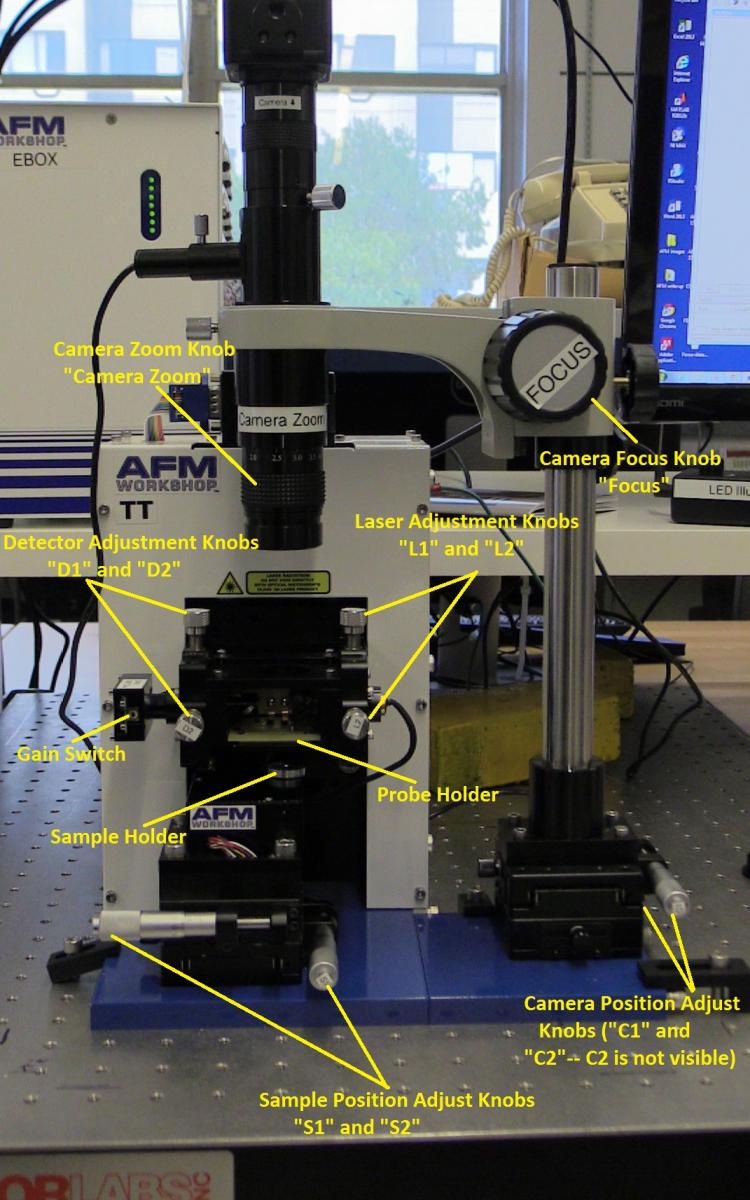
\includegraphics[width=\linewidth,keepaspectratio]{images/AFMgen.jpg}}
  \caption{AFM Apparatus \\ \href{http://experimentationlab.berkeley.edu/sites/default/files/AFMImages/AFMgen.jpg}{Click here to see larger picture}}
  \label{fig:Apparatus}
\endminipage\hfill
\minipage{0.32\textwidth}
  \href{http://experimentationlab.berkeley.edu/sites/default/files/AFMImages/bothfocused.JPG}{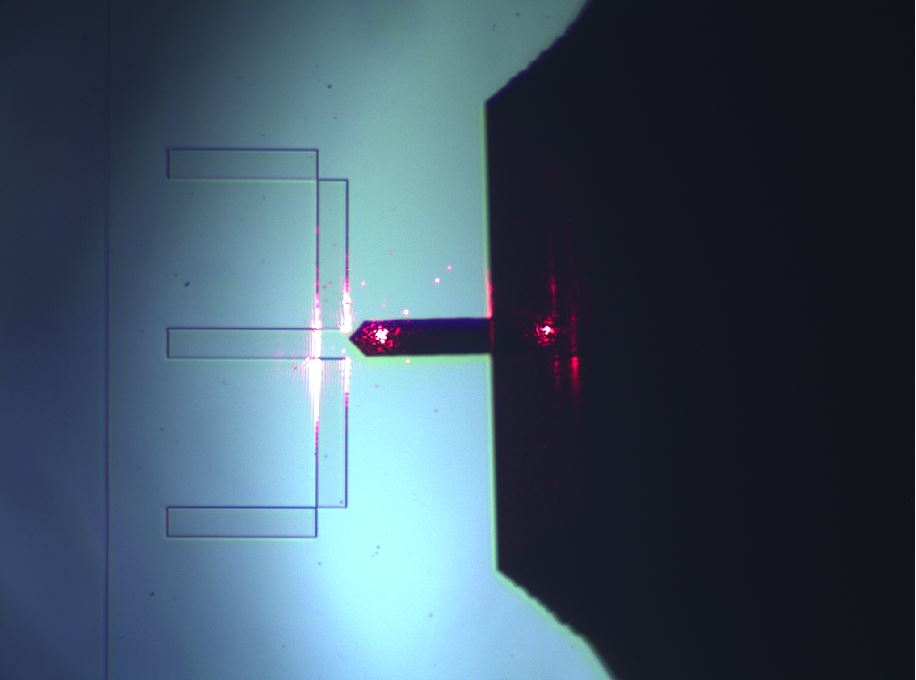
\includegraphics[width=\linewidth,keepaspectratio]{images/bothfocused2.jpg}}
  \caption{Laser focused on cantilever \\
  \href{http://experimentationlab.berkeley.edu/sites/default/files/AFMImages/bothfocused.JPG}{Click here to see larger picture}}
  \label{fig:CantileverLaser}
\endminipage\hfill
\minipage{0.32\textwidth}
  \href{http://experimentationlab.berkeley.edu/sites/default/files/AFMImages/AFMstation.jpg}{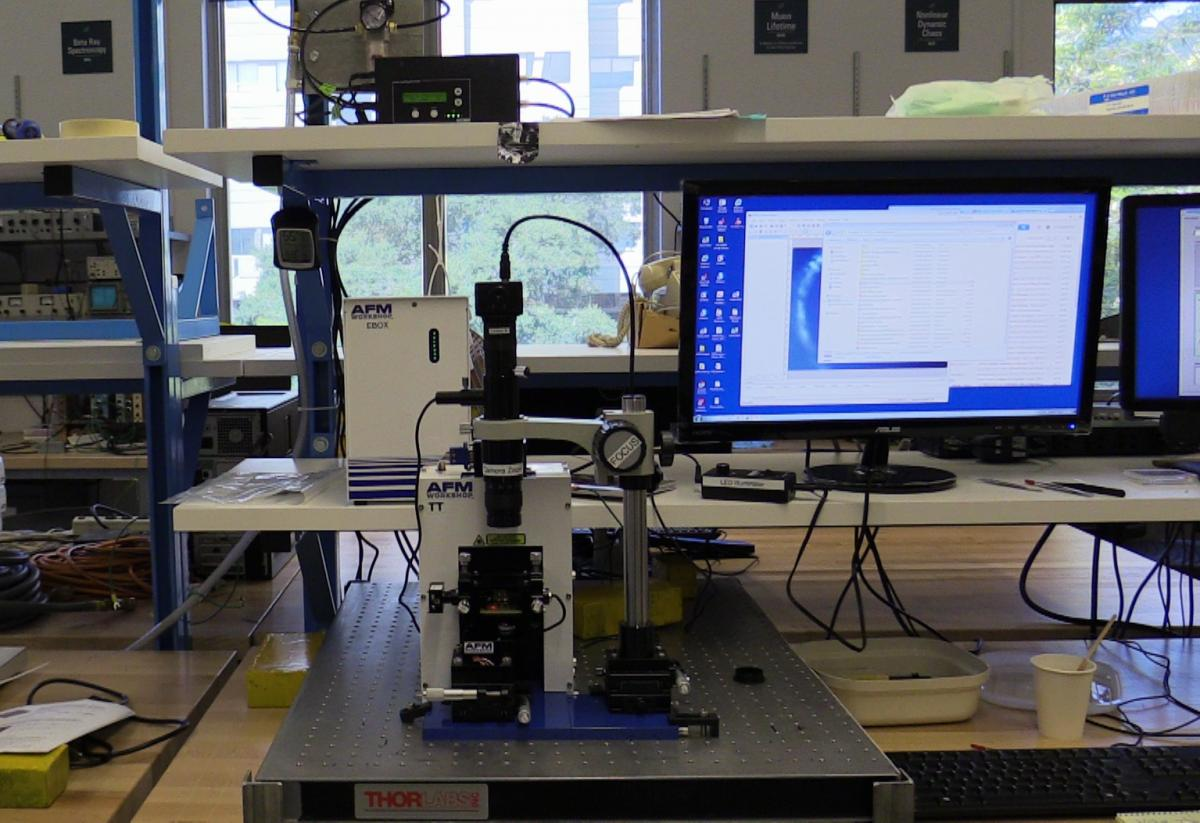
\includegraphics[width=\linewidth,keepaspectratio]{images/AFMstation.jpg}}
  \caption{AFM on level stage \\ \href{http://experimentationlab.berkeley.edu/sites/default/files/AFMImages/AFMstation.jpg}{Click here to see larger picture}}\label{fig:LevelStage}
\endminipage
\end{figure}

\begin{figure}[!h]
\minipage{0.32\textwidth}
  \href{http://experimentationlab.berkeley.edu/sites/default/files/AFMImages/9.JPG}{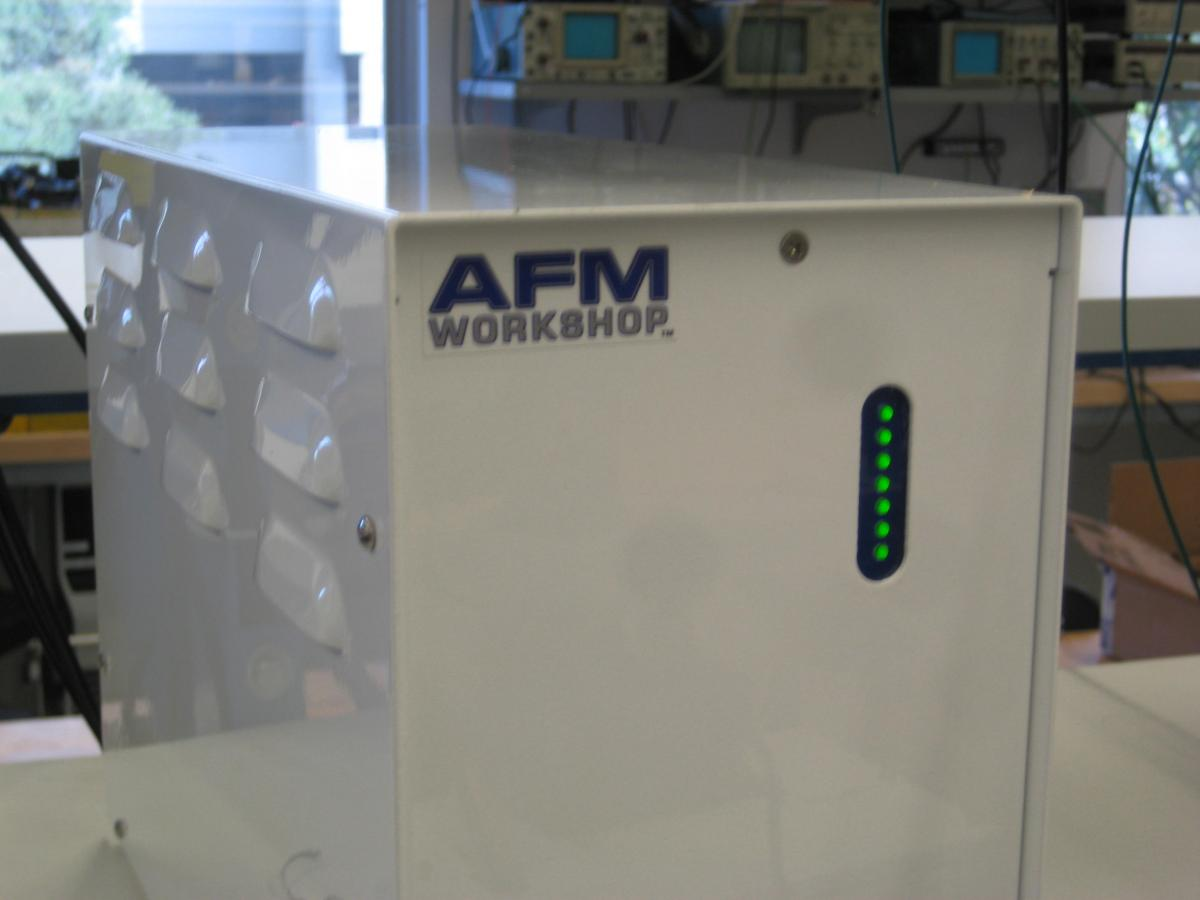
\includegraphics[width=\linewidth,keepaspectratio]{images/9.JPG}}
  \caption{AFM EBOX\\ \href{http://experimentationlab.berkeley.edu/sites/default/files/AFMImages/9.JPG}{Click here to see larger picture}}
  \label{fig:AFMEBox}
\endminipage\hfill
\minipage{0.32\textwidth}
  \href{http://experimentationlab.berkeley.edu/sites/default/files/AFMImages/toposcan.JPG}{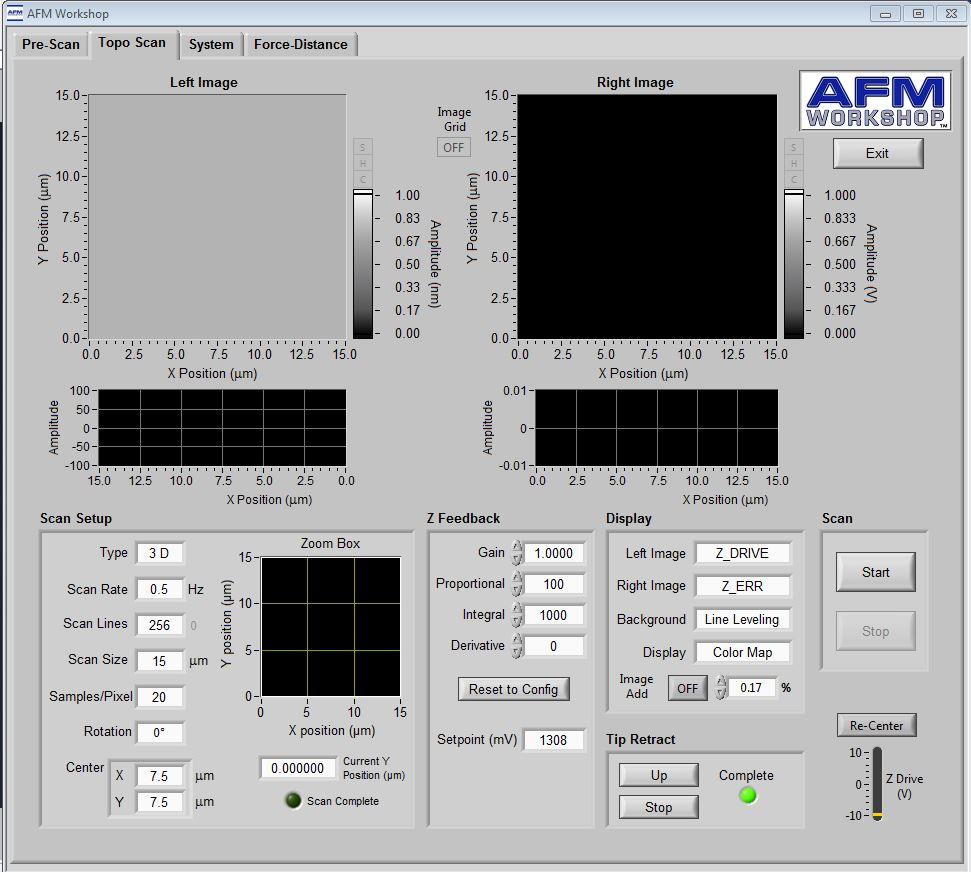
\includegraphics[width=\linewidth,keepaspectratio]{images/toposcan.JPG}}
  \caption{Topographic scan window \\
  \href{http://experimentationlab.berkeley.edu/sites/default/files/AFMImages/toposcan.JPG}{Click here to see larger picture}}
  \label{fig:TopoScan}
\endminipage\hfill
\minipage{0.32\textwidth}
  \href{http://experimentationlab.berkeley.edu/sites/default/files/AFMImages/LED2.jpg}{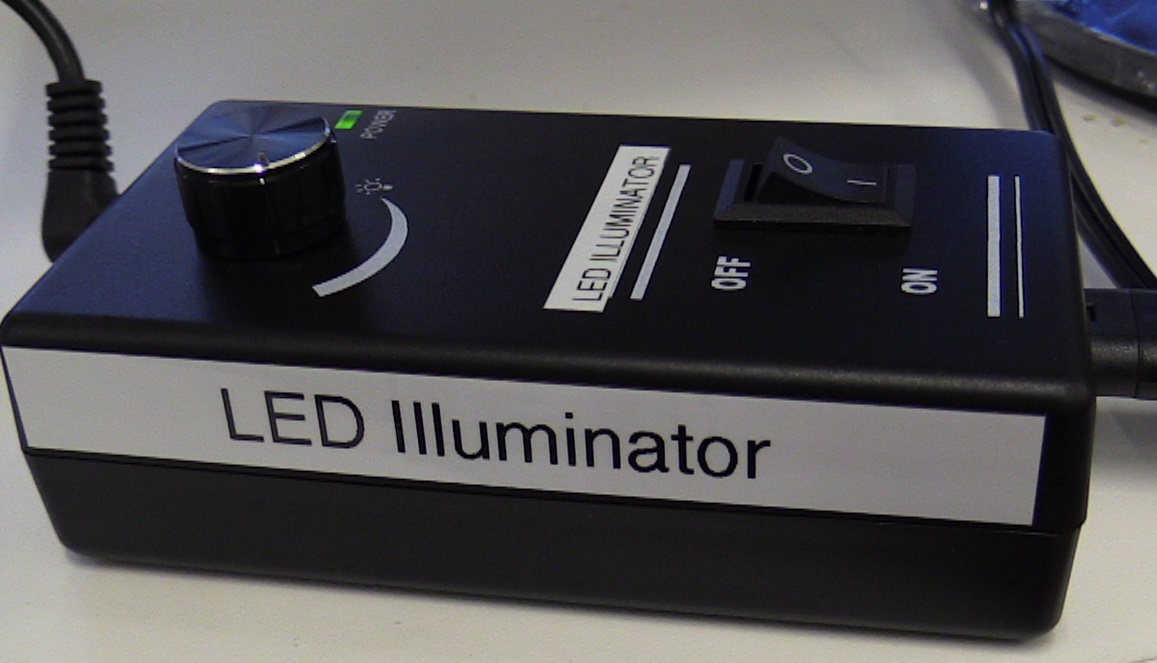
\includegraphics[width=\linewidth,keepaspectratio]{images/LED2.jpg}}
  \caption{Illuminator \\ \href{http://experimentationlab.berkeley.edu/sites/default/files/AFMImages/LED2.jpg}{Click here to see larger picture}}\label{fig:Illuminator}
\endminipage
\end{figure}

\section{Before the 1st Day of Lab }

\begin{enumerate}
    \item Watch the \href{http://experimentationlab.berkeley.edu/sites/default/files/Introduction\%20Video\_2.mp4}{\textbf{AFM Basics}} introductory video

    \item \emph{Print out the checkpoints page. Checkpoints are examination points where you must STOP and get a GSI or professor to verify your understanding and/or verify proper experimental setup. You cannot skip the checkpoints, as there is a \href{http://experimentationlab.berkeley.edu/node/136}{\textbf{sign off sheet}} that must be scanned in with your lab report. Print out the checkpoints page now and look it over.}

    \item Review \href{http://experimentationlab.berkeley.edu/sites/default/files/AFMImages/Lecture\_10\_AFM.pdf}{\textbf{Lecture 10}} (a PowerPoint presentation) which gives a brief overview of AFM history and background and basic operation.

    \item Read \textbf{Chapter 1} Introduction to \href{http://experimentationlab.berkeley.edu/afm-book}{\textbf{Atomic Force Microscopy}} by Peter Eaton and Paul West. Skim \textbf{Chapter 2} Instrumentation and \textbf{Chapter 3} Modes.

    \item Read through this entire experiment lab manual.

    \item Complete the \href{http://experimentationlab.berkeley.edu/node/122}{\textbf{AFM Pre-lab}} and Evaluation sheet. Print, fill it out with the answers, and turn it in with your report. The Pre-Lab must be printed separately. Discuss the experiment and pre-lab questions and answers with any faculty member or GSI and get it signed off by that faculty member or GSI. Turn in the signed pre-lab sheet with answers with your lab report.

\end{enumerate}

\textbf{Animations \& Videos}

\begin{itemize}
    \item C:/AFM Experiment/animations

    \begin{itemize}
        \item This folder contains 40 animations which are each just a few seconds long, demonstrating different concepts about the AFM

    \end{itemize}

    \item C:/AFM Experiment/Instructional Videos

    \begin{itemize}
        \item Shows quick tutorials on how to operate this AFM, but leaves out a lot of details and troubleshooting

        \item Follow AFM Workshop \href{http://experimentationlab.berkeley.edu/tt-afmuserguidev2.2}{\textbf{TT-AFM Users Guide}} and the  lab manual

        \item Last day of the experiment please fill out the \href{\ExperimentEvaluation}{\textbf{Experiment Evaluation}}

    \end{itemize}

\end{itemize}

\textbf{Suggested Reading}

\begin{itemize}
    \item PDFs located in the C:/AFM Experiment/Articles PDFs

    \item \href{http://experimentationlab.berkeley.edu/afm-book}{\textbf{Atomic Force Microscopy}} by Peter Eaton and Paul West (It's a book)
    \begin{itemize}
        \item We have the online link to the book linked below.  You can also find the book in C:/AFM Experiment/Book

        \begin{itemize}
            \item \textbf{Chapter 1} Introduction (required above)

            \item \textbf{Chapter 2} Instrumentation

            \item \textbf{Chapter 3} Modes

            \item \textbf{Chapter 4} Measuring AFM Images

            \item \textbf{Chapter 5} Image Processing and analysis

            \item \textbf{Chapter 6} Image Artifacts (suggested)

            \item \textbf{Chapter 7} Applications of AFM

            \item \textbf{Appendix-B} Scanner-Calibration procedure

        \end{itemize}

    \end{itemize}

\end{itemize}

\textbf{References}

\begin{itemize}
    \item AFM Workshop \href{http://experimentationlab.berkeley.edu/tt-afmuserguidev2.2}{\textbf{TT-AFM Users Guide V 2.2}} (it's actually quite helpful)

    \item See the paper, \href{http://experimentationlab.berkeley.edu/sites/default/files/AFMImages/butt\_AFM.pdf}{\textbf{Butt\_AFM}} for force distance information.  See pg 28 for Figure 9, showing the laser reflecting off of the cantilever onto the detector.  Also see pg 30-32 for a discussion of the analysis of Force Distance Curves.

    \item Note: Some photos on this page are from \href{http://www.afmworkshop.com/}{\textbf{AFMworkshop}} where this apparatus was purchased.

\end{itemize}

\section{Objectives}

\begin{itemize}
    \item Gain experience with extremely delicate and sensitive equipment

    \item Study how the environmental noise affects measurements

    \item Learn how to align, calibrate, and operate an Atomic Force Microscope (AFM)

    \item Learn to use Gwyddion, a free scanning probe microscopy (SPM) data visualization and analysis software

    \item Conduct experiments in which you take multiple scans of different samples and learn how to process and analyze the images produced by the AFM using the software Gywddion.  The experiments you will conduct include:

    \begin{itemize}
        \item Measure the Noise Floor and determine the error due to noise

        \item Determine the spring constant of your probe, and measure Boltzmann's Constant

        \item Analyze the Force Distance Curves produced by the AFM software as the probe approaches and withdraws from a sample.

        \item Take a topographical and phase scan of a glue stick to study its topography and map it's surface hardness.

        \item Take a topographical scan of a CD and DVD and determine their properties.

        \item Take a topographical scan of a MicroCircuit and determine its properties.

    \end{itemize}

\end{itemize}

\section{Introduction}

In this lab, you will operate an atomic force microscope which is used to image 3D surfaces on the angstrom to micron level. AFM is relatively inexpensive and is used across many different fields of science including physics, chemistry, and biology.

\textbf{What is an Atomic Force Microscope?}

An atomic force microscope images objects on the scale of angstroms to microns through the use of physical scanning, rather than optics (like conventional/electron microscopes). The basic mechanism of the AFM is shown in Figure~\ref{fig:BasicMechanism}. A tip attached to a cantilever interacts with a surface. A laser is bounced off of the cantilever and into a photodetector. From this signal, one measures the deflection of the cantilever. A sample is then placed on a special stage underneath the tip. The stage contains a \hyperref[subsubsec:Piezo]{piezoelectric} driver that is controlled by software. In particular, it may be made to wiggle around in a raster scan pattern, as well as engage in feedback with the cantilever (constant force mode). Variations in the height of the sample cause deflections of the cantilever, which are then picked up by the photodetector. Through this lab, you should gain a good understanding of how an AFM works, the types of data you can get from it, how you can use this data to make meaningful conclusions, and the limitations of the system.

\textbf{Why AFM over other microscopy techniques?}
\begin{itemize}
    \item Take images in all environments (air, liquid, vacuum)

    \item Interaction with the surface allows for measurements of surface physical properties

    \item The sample need not be conductive (compare to STM)

    \item Examples of surface features that may be imaged include: atomic terraces, carbon nanotubes, colloidal particles, viruses, DVD textures up to micro lens textures, fractured surfaces, and complex multi-phase polymers

    \item AFM can deliver 3D topography info from the angstrom level to the micron scale

    \item Very high vertical resolution (AFM have imaged individual atoms)

    \item Can manipulate surface features (nanolithography), given a magnetic or specially hardened tip (ours is not equipped for this)

\end{itemize}

\begin{figure}[h]
    \centering
    \href{http://experimentationlab.berkeley.edu/sites/default/files/AFMImages/2_0.png}{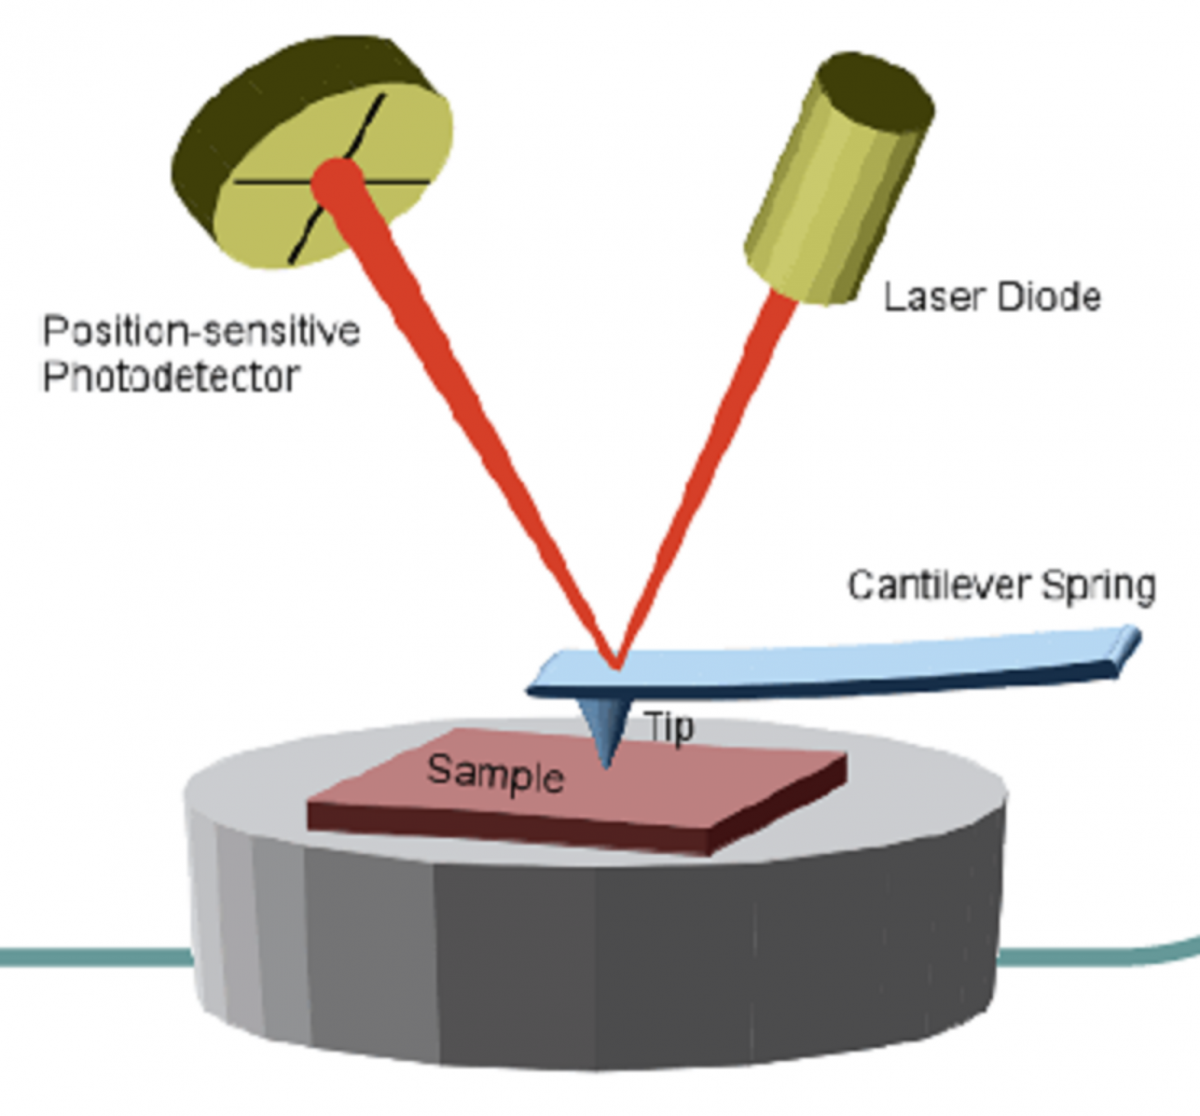
\includegraphics[width=0.5\linewidth]{images/2_0.png}}
    \caption{Diagram of the laser reflecting off the cantilever surface. The deflection of the cantilever as the tip moves across the surface of the sample is measured by the deflection of the laser reflecting onto the photodetector, and this data is used to adjust the position of the cantilever to recenter the beam.}
    \label{fig:BasicMechanism}
\end{figure}

\subsection{Apparatus}

\begin{figure}[h]
\centering
    \href{http://experimentationlab.berkeley.edu/sites/default/files/AFMImages/AFMgen.jpg}{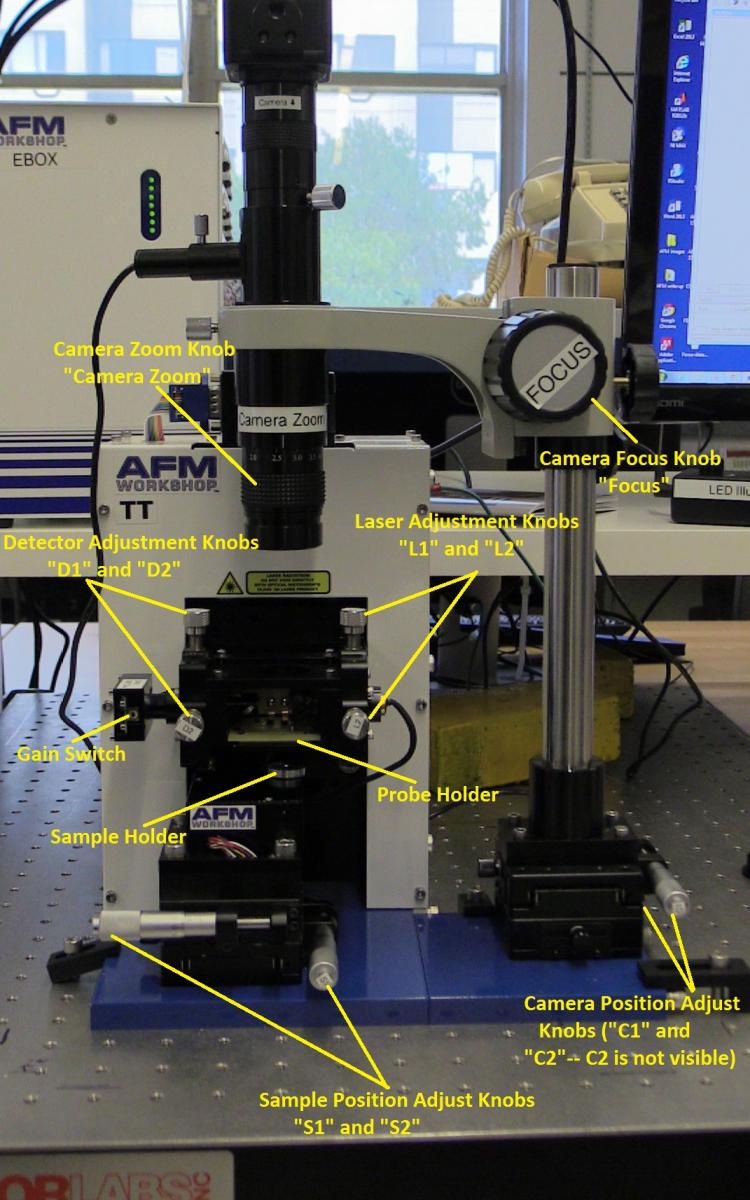
\includegraphics[width=0.25\linewidth]{images/AFMgen.jpg}}
    \caption{AFM Apparatus. Click \href{http://experimentationlab.berkeley.edu/sites/default/files/AFMImages/AFMgen.jpg}{\textbf{here}} for a larger image.}
\end{figure}

\textbf{Probe:}

AFM probes are extremely fragile, so you must handle them with extreme care throughout this experiment. Each probe cost about \$30, so keep this in mind when you do this experiment.

See the \href{http://experimentationlab.berkeley.edu/sites/default/files/AFMImages/ACLA\_4\_datasheet.pdf}{\textbf{datasheet}} for the AFM probes. \href{http://experimentationlab.berkeley.edu/sites/default/files/AFMImages/1.1.\%20Generating\%20an\%20image.flv\_converted.mp4}{\textbf{Here}} is an animation showing the probe interacting with the surface of a sample.

\begin{figure}[!h]
\minipage{0.49\textwidth}
  \href{http://experimentationlab.berkeley.edu/sites/default/files/AFMImages/AFMprobe.JPG}{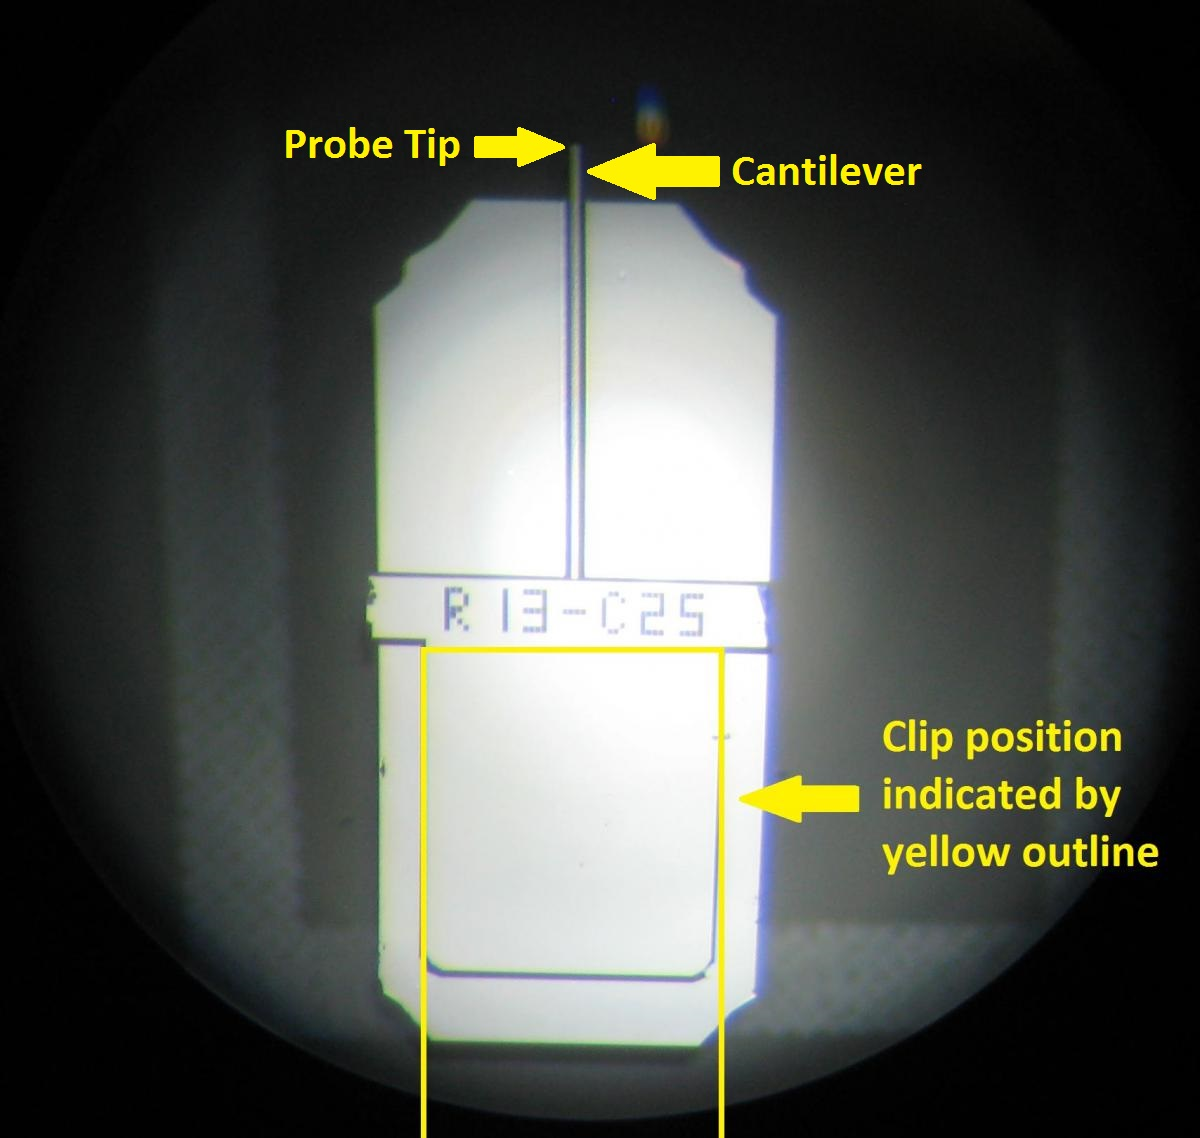
\includegraphics[width=\linewidth,keepaspectratio]{images/AFMprobe.JPG}}
  \caption{AFM probe bottom view}
  \label{fig:AFMProbe}
\endminipage\hfill
\minipage{0.49\textwidth}
  \href{http://experimentationlab.berkeley.edu/sites/default/files/AFMImages/26.png}{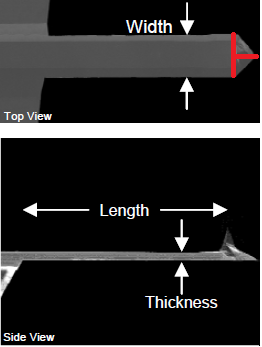
\includegraphics[width=\linewidth,keepaspectratio]{images/26.png}}
  \caption{AFM probe top and side view}
  \label{fig:AFMProbe2}
\endminipage
\end{figure}

Imagine a crosshair at the triangle point of the cantilever. That is roughly where your tip is located.

\textbf{Probe animations:}

\begin{itemize}
    \item \href{http://experimentationlab.berkeley.edu/sites/default/files/AFMImages/5.2.\%20Probe\%20Shape\%20-\%20Hole.flv\_converted.mp4}{\textbf{Shape of the probe}}

    \item \href{http://experimentationlab.berkeley.edu/sites/default/files/AFMImages/5.1\%20Contamination.flv\_converted.mp4}{\textbf{Tip interacting with contamination}} present on samples

    \item \href{http://experimentationlab.berkeley.edu/sites/default/files/AFMImages/5.3.\%20Probe\%20Sample\%20Bump.flv\_converted.mp4}{\textbf{Probe interacting with sample}}

\end{itemize}

\textbf{What is the Piezoelectric Effect?}
\label{subsubsec:Piezo}

The Piezoelectric Effect is the ability of certain materials to generate an electric charge in response to applied mechanical stress. The word Piezoelectric is derived from the Greek piezein, which means to squeeze or press, and piezo, which is Greek for “push”.

One of the unique characteristics of the piezoelectric effect is that it is reversible, meaning that materials exhibiting the direct piezoelectric effect (the generation of electricity when stress is applied) also exhibit the converse piezoelectric effect (the generation of stress when an electric field is applied).

When piezoelectric material is placed under mechanical stress, a shifting of the positive and negative charge centers in the material takes place, which then results in an external electrical field. When reversed, an outer electrical field either stretches or compresses the piezoelectric material.

The piezoelectric effect is very useful within many applications that involve the production and detection of sound, generation of high voltages, electronic frequency generation, microbalances, and ultra-fine focusing of optical assemblies. It is also the basis of a number of scientific instrumental techniques with atomic resolution, such as scanning probe microscopes (STM, AFM, etc). The piezoelectric effect also has its use in more mundane applications as well, such as acting as the ignition source for cigarette lighters. 

\textbf{Detector and Feedback Loop:}

\begin{itemize}
    \item \href{http://experimentationlab.berkeley.edu/sites/default/files/AFMImages/2.1.\%20photodetector.flv\_converted.mp4}{\textbf{Here}} is an animation of how the detector outputs a voltage proportional to the surface topography of a sample.

    \item A light lever is created by reflecting the light off of the cantilever.  \href{http://experimentationlab.berkeley.edu/sites/default/files/AFMImages/2.3.\%20Light\%20Lever.flv\_converted.mp4}{\textbf{Here}} is a quick animation showing the operation of the light lever. Do you see how T-B, the signal on photodetector T minus the signal from photodetector B, gives the relative vertical deflection of the cantilever?
    \begin{figure}[h]
        \centering
        \href{http://experimentationlab.berkeley.edu/sites/default/files/AFMImages/AFMlasermirror.png}{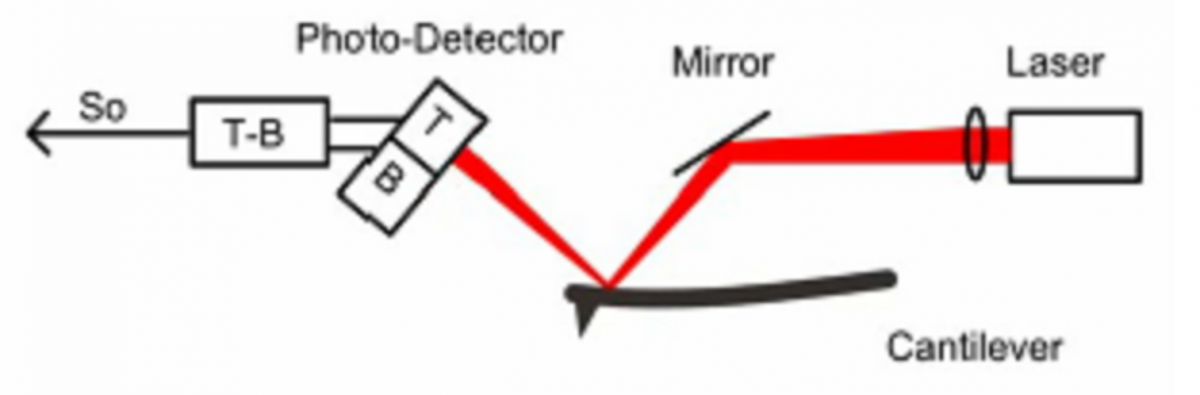
\includegraphics[width=0.5\linewidth]{images/AFMlasermirror.png}}
        \caption{Laser-Mirror Setup}
        \label{fig:AFMlasermirror}
    \end{figure}

    \item Piezoelectric Ceramics:  A material which expands when a voltage is applied.  They have very precise motion control ($<$ .01 nm).  This \href{http://experimentationlab.berkeley.edu/sites/default/files/AFMImages/3.1.\%20Motion.flv\_converted.mp4}{\textbf{animation}}, and this other \href{http://experimentationlab.berkeley.edu/sites/default/files/AFMImages/3.2.\%20proportional.flv\_converted.mp4}{\textbf{animation}}, show how piezos work.

    \item The motion of the \href{http://experimentationlab.berkeley.edu/sites/default/files/AFMImages/3.3.\%20Y\%20Scanner\_converted.mp4}{\textbf{y piezo}} is shown in this animation.

    \item This \href{http://experimentationlab.berkeley.edu/sites/default/files/AFMImages/3.4.\%20Z\%20Scanner.flv\_converted.mp4}{\textbf{animation}} and this\textbf{ }\href{http://experimentationlab.berkeley.edu/sites/default/files/AFMImages/4.1.\%20Z\%20motion.flv\_converted.mp4}{\textbf{animation}} show how the z piezo works.

    \item Stage Integration:
    
    \begin{figure}[!h]
\minipage{0.4\textwidth}
  \href{http://experimentationlab.berkeley.edu/sites/default/files/AFMImages/AFMdiagram.png}{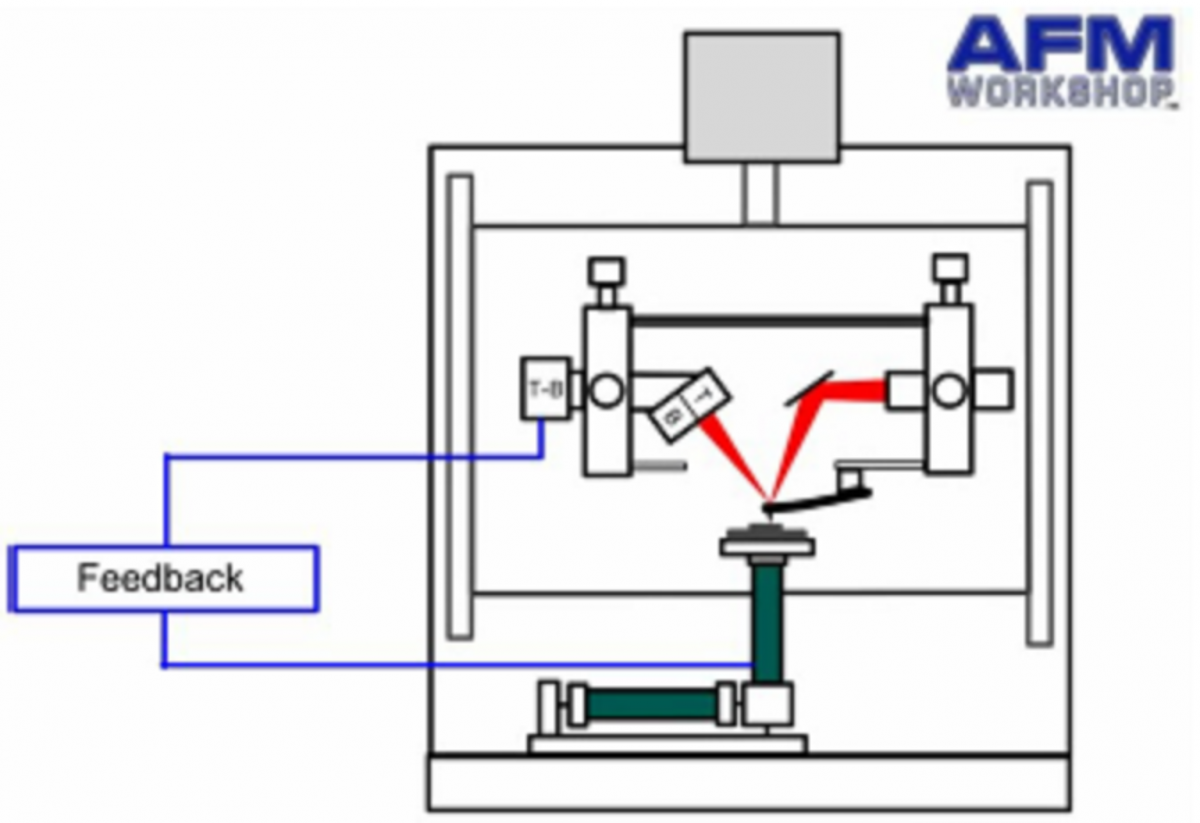
\includegraphics[width=\linewidth,keepaspectratio]{images/AFMdiagram.png}}
  \caption{Piezo integration}
  \label{fig:PiezoIntegration}
\endminipage\hfill
\minipage{0.58\textwidth}
  \href{http://experimentationlab.berkeley.edu/sites/default/files/AFMImages/AFMstage2.PNG}{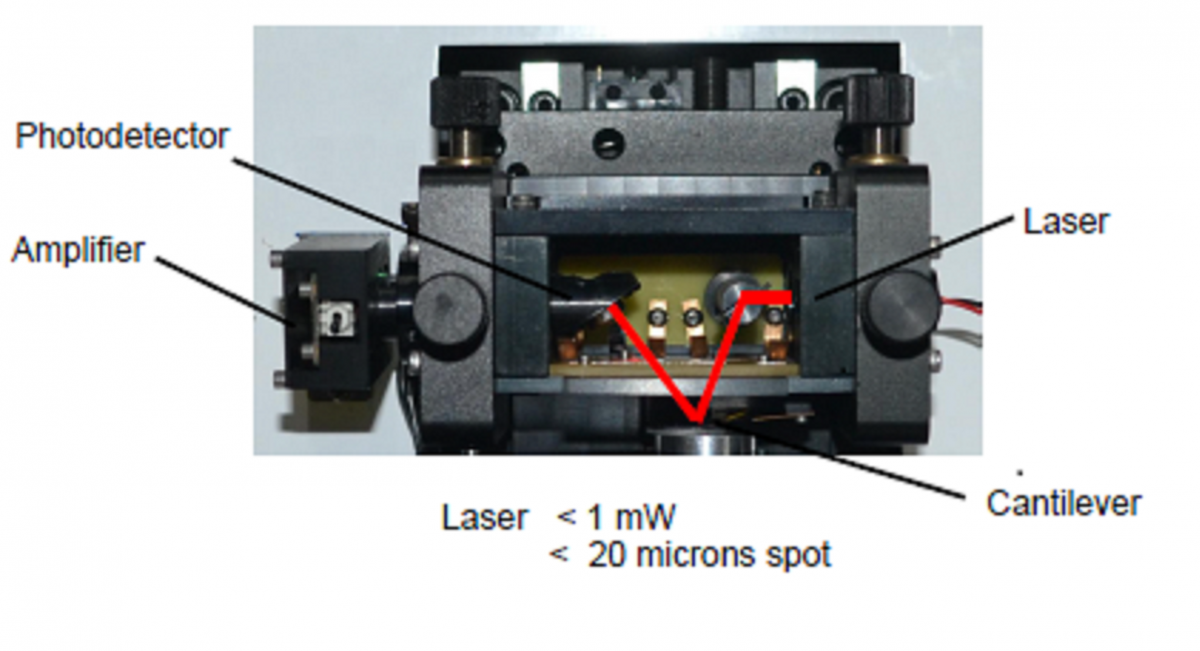
\includegraphics[width=\linewidth,keepaspectratio]{images/AFMstage2.PNG}}
  \caption{Laser Setup}
    \label{fig:LaserSertup}
\endminipage
\end{figure}

\end{itemize}

\pagebreak

\textbf{Mechanism:}

The sample stage scans around in a raster pattern underneath the probe. When the probe encounters a surface feature (a bump or whatever), the cantilever bends. This changes the position of the laser on the photodetectors. The T-B signal is recorded by the software. In ``feedback mode,'' the T-B signal is an error signal applied to the sample stage's z piezo. The feedback mechanism works to keep the deflection of the cantilever at a minimum. In this case, the feedback signal gives all of the information about the surface.

\textbf{Ebox:}

The EBOX is located on the shelf behind the AFM. The EBOX houses the DAQ and connects/interfaces the AFM hardware with the software on the computer.

\begin{figure}[!h]
\minipage{0.49\textwidth}
  \href{http://experimentationlab.berkeley.edu/sites/default/files/EBOX.jpg}{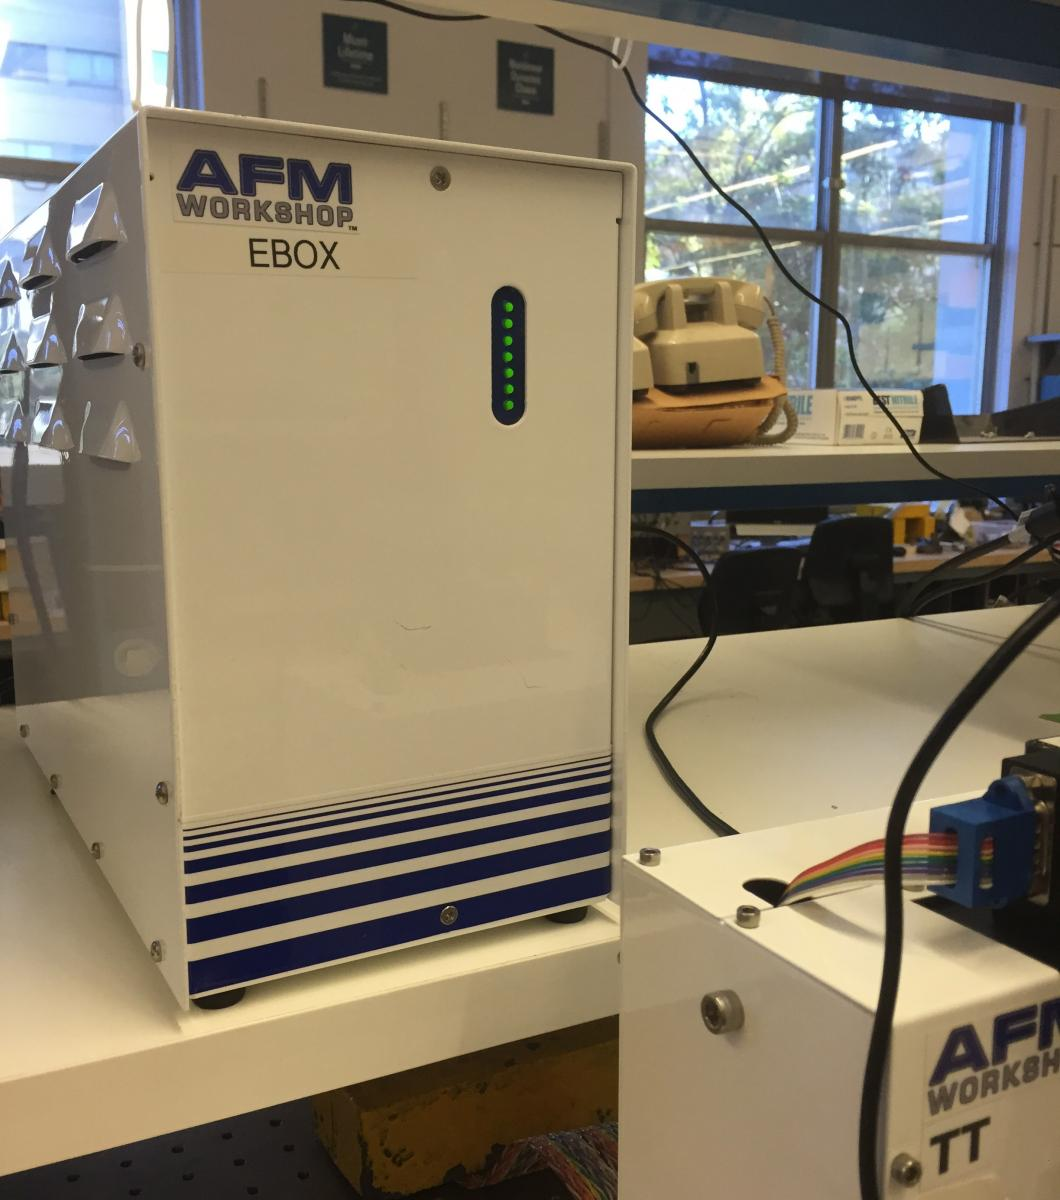
\includegraphics[width=\linewidth,keepaspectratio]{images/EBOX.jpg}}
  \caption{AFM EBOX}
  \label{fig:EBox}
\endminipage\hfill
\minipage{0.49\textwidth}
  \href{http://experimentationlab.berkeley.edu/sites/default/files/AFMImages/AFMconnections.PNG}{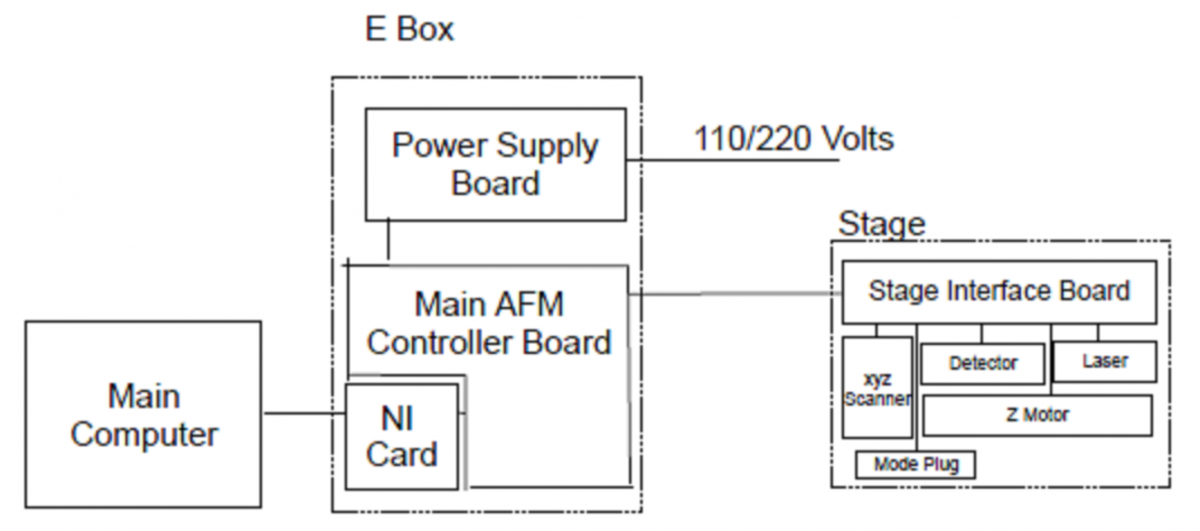
\includegraphics[width=\linewidth,keepaspectratio]{images/AFMconnections.PNG}}
  \caption{AFM Connections}
    \label{fig:AFMConnections}
\endminipage
\end{figure}

\subsection{Software}

\textbf{Note: If you are experiencing bugs with the software, refer to the} \hyperref[sec:Troubleshooting]{Troubleshooting Section} \textbf{at the end of this lab}

The software controls the AFM mechanisms and exports collected data as a .wsf file. In particular, it controls the motion of the sample stage, automates the tip approach, measures the resonance frequency of the cantilever for ``vibrating mode'' (see below), and collects the data from the photo detector.

Use this section as a reference for when you calibrate the AFM and scan.

\textbf{Tip Approach}:  Later, after you load the sample, and adjust various parameters in the AFM program, you will lower the tip to the sample using the \hyperref[subsec:TipApproach]{Automated Tip Approach}.  When the Automated Tip Approach has lowered the tip all the way down to the surface, it will indicate that it is ``In Feedback.'' Here is an animation demonstrating \href{http://experimentationlab.berkeley.edu/sites/default/files/AFMImages/4.4.\%20feedback.flv\_converted.mp4}{\textbf{Feedback}}.

\begin{figure}[h]
    \centering
    \href{http://experimentationlab.berkeley.edu/sites/default/files/AFMImages/infeedback.JPG}{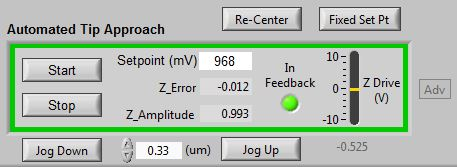
\includegraphics[width=0.5\linewidth]{images/infeedback.JPG}}
    \label{fig:infeedback}
\end{figure}

\textbf{Prescan Tab}: Where you will select mode (if vibrating mode, you will also find the resonant frequency), perform a \hyperref[subsubsec:RangeCheck]{range check}, and engage the \hyperref[subsec:TipApproach]{tip with the sample}.

\begin{figure}[h]
    \centering
    \href{http://experimentationlab.berkeley.edu/sites/default/files/AFMImages/prescantab.JPG}{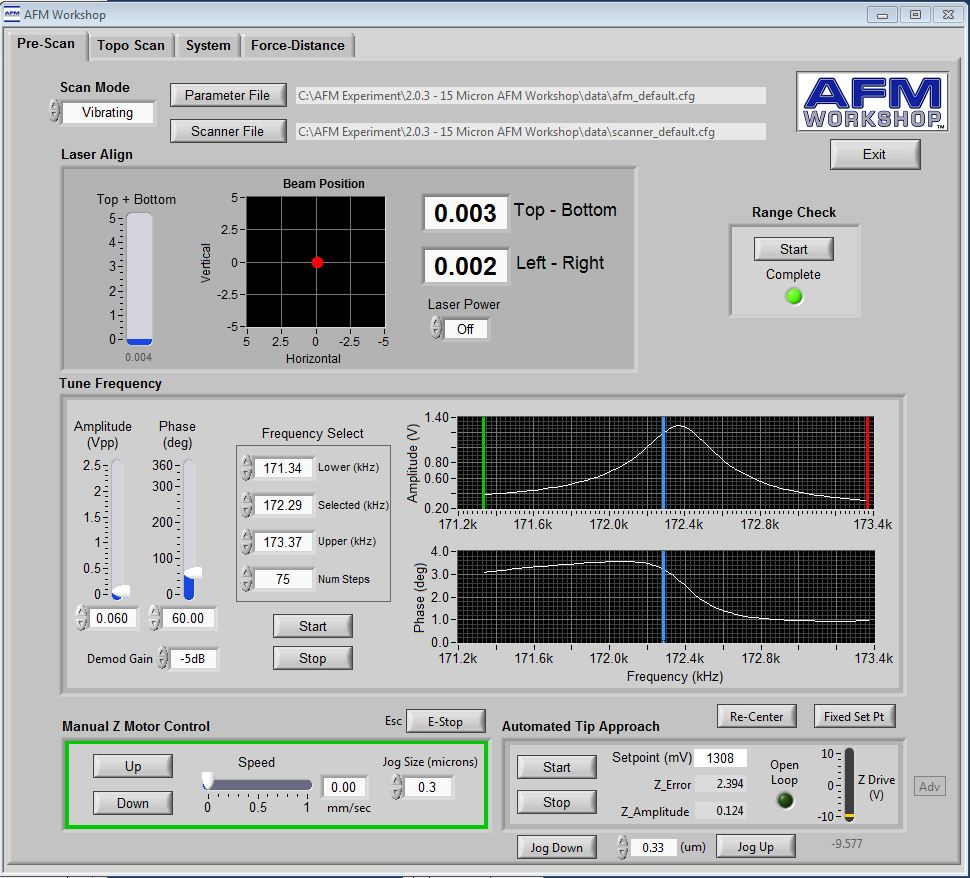
\includegraphics[width=0.5\linewidth]{images/prescantab.JPG}}
    \label{fig:prescantab}
\end{figure}

\subsection{Scanning Modes}

\begin{itemize}
    \item Vibrating vs. Non-vibrating Mode

    \begin{itemize}
        \item In \href{http://experimentationlab.berkeley.edu/sites/default/files/AFMImages/7.2.\%20tip\%20sample\%20Vibrating.flv\_converted.mp4}{\textbf{vibrating mode}}, a piezo driver (not the sample stage piezo!) vibrates the cantilever at frequency slightly below its resonance frequency. The amplitude of the oscillation is kept approximately constant through feedback.  The tip strikes against the surface and detaches from the sample surface on each oscillation cycle by using a large vibration amplitude, overcoming meniscus forces (see below: Atomic Interaction) and loss in lateral resolution.  As the tip approaches a sample, the van der Waals attractive force between the tip and the sample causes changes in both the amplitude and the phase of the cantilever vibration.  As it passes over a surface, changes in the cantilever's vibrations correlate to topographical features.

        \item In non-vibrating mode, the probe is always in contact with the surface, and is dragged along the sample to create the image.  Non-Vibrating mode is used when you are measuring a force-distance curve and when measuring Boltzmann's constant. In ``Constant Force Mode'' (see below), the Z Piezo (the vertical position of the cantilever/probe) uses the feedback signal to adjust its height in such a way as to hold the deflection of the cantilever constant.
    \end{itemize}

    \item Non-vibrating scanning modes: constant height and constant force

    \begin{itemize}
        \item Constant Height (No feedback):

        \begin{itemize}
            \item In this mode, the spatial variation of the cantilever deflection is used directly to generate the topographic data set because the height of the scanner is fixed as it scans.

            \item Constant-height mode is often used for taking atomic-scale images of atomically flat surfaces, where the cantilever deflections and thus variations in applied force are \textbf{small}.

            \item Constant-height mode is also essential for recording real-time images of changing surfaces, where high scan speed is essential.

        \end{itemize}

        \item Constant Force:

        \begin{itemize}
            \item In this mode, the deflection of the cantilever can be used as input to a feedback circuit that moves the scanner up and down in \textbf{z}, responding to the topography by keeping the cantilever deflection constant.

            \item With the cantilever deflection held constant, the total force applied to the sample is constant.

            \item In this mode, the image is generated from the scanner's z-motion. The scanning speed is thus limited by the response time of the feedback circuit.

        \end{itemize}

    \end{itemize}

    \item Resonance Frequency: The cantilever acts like a simple harmonic oscillator. The resonance frequency of the cantilever determines the frequency we use in vibrating mode (we drive it at 80 percent of the resonance to prevent damage). \href{http://experimentationlab.berkeley.edu/sites/default/files/AFMImages/2.1.1.\%20Intro\%20Vibrating\%20Cantf.swf.mp4}{\textbf{Here}} is a quick animation showing the oscillation of the cantilever.

    \item Phase (deg): The phase of cantilever oscillations.  There should be an inflection point in phase at the point of resonance. (see screenshot above) Phase shifts in the cantilever signal also give information about surface features.

    \item Automated Tip Approach:  the mechanism by which the AFM software slowly lowers the probe tip to within a few nanometers of the sample's surface.  The AFM program uses a ``Woodpecker'' Tip Approach, demonstrates in the image below: The \href{http://experimentationlab.berkeley.edu/sites/default/files/AFMImages/VM\%203.3.\%20Avg\%20Dist\%20Control\_converted.mp4}{\textbf{setpoint}} determines the amount of deflection that the feedback attempts to maintain.
    
    \begin{figure}[h]
    \begin{center}
        \href{http://experimentationlab.berkeley.edu/sites/default/files/AFMImages/AFMwoodpecker.png}{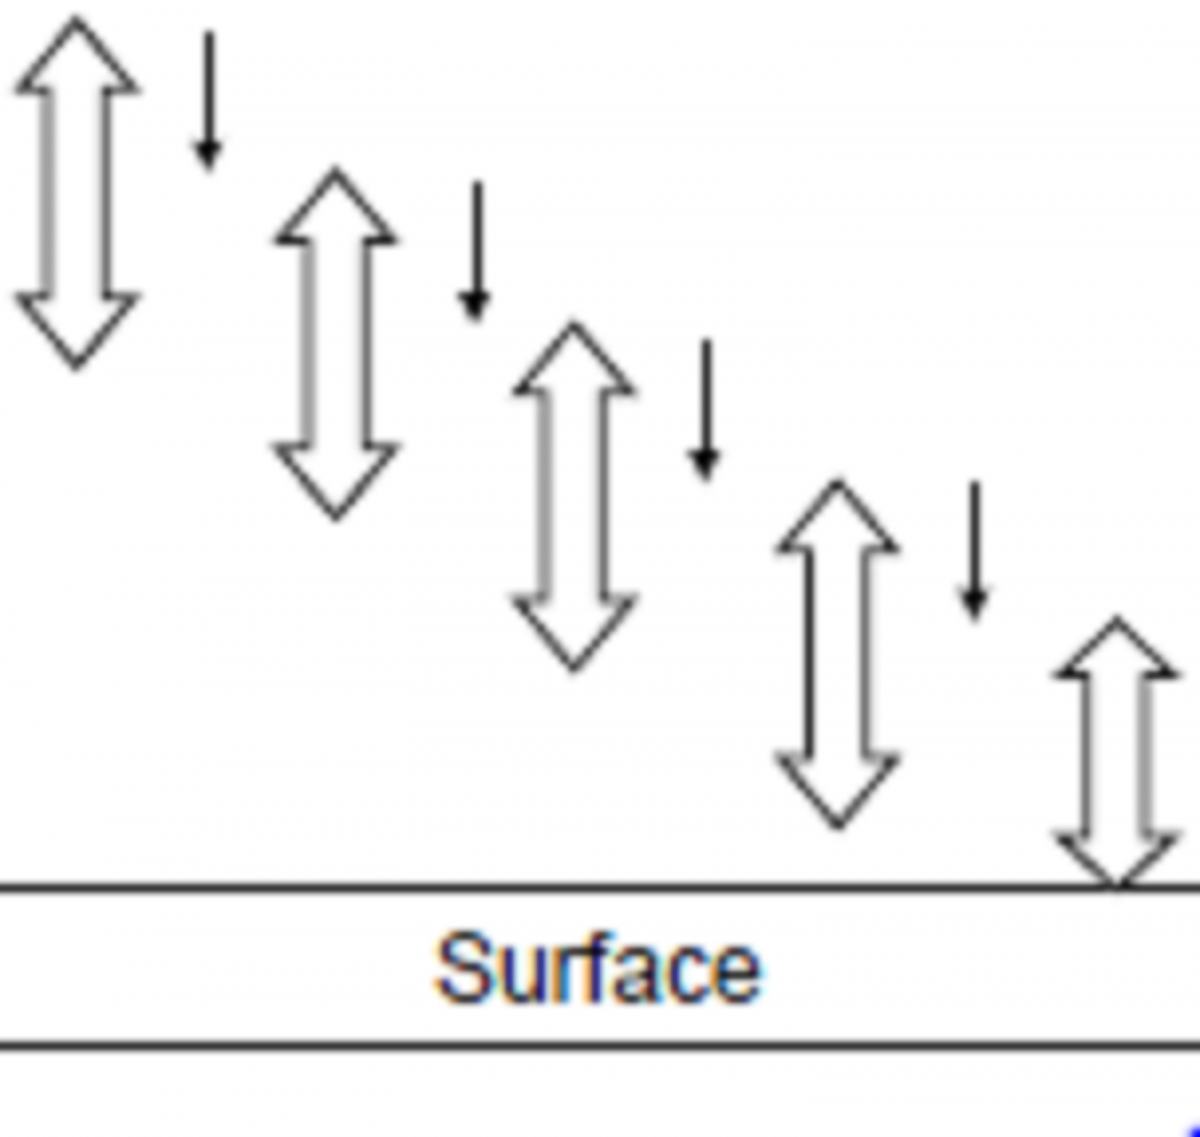
\includegraphics[width=0.3\linewidth]{images/AFMwoodpecker.png}}
        \caption{Woodpecker tip approach}
        \label{Woodpecker}
    \end{center}
    \end{figure}

\end{itemize}

\textbf{Topo Scan Tab} - Where you can adjust scan parameters like scan speed, scan size, what measurements you want to take (i.e. Z Drive will give basic topography, Z phase will give hardness, and Z error will map abrupt changes in topography). A screenshot of the tab is shown below:

\begin{center}
    \href{http://experimentationlab.berkeley.edu/sites/default/files/AFMImages/toposcan.JPG}{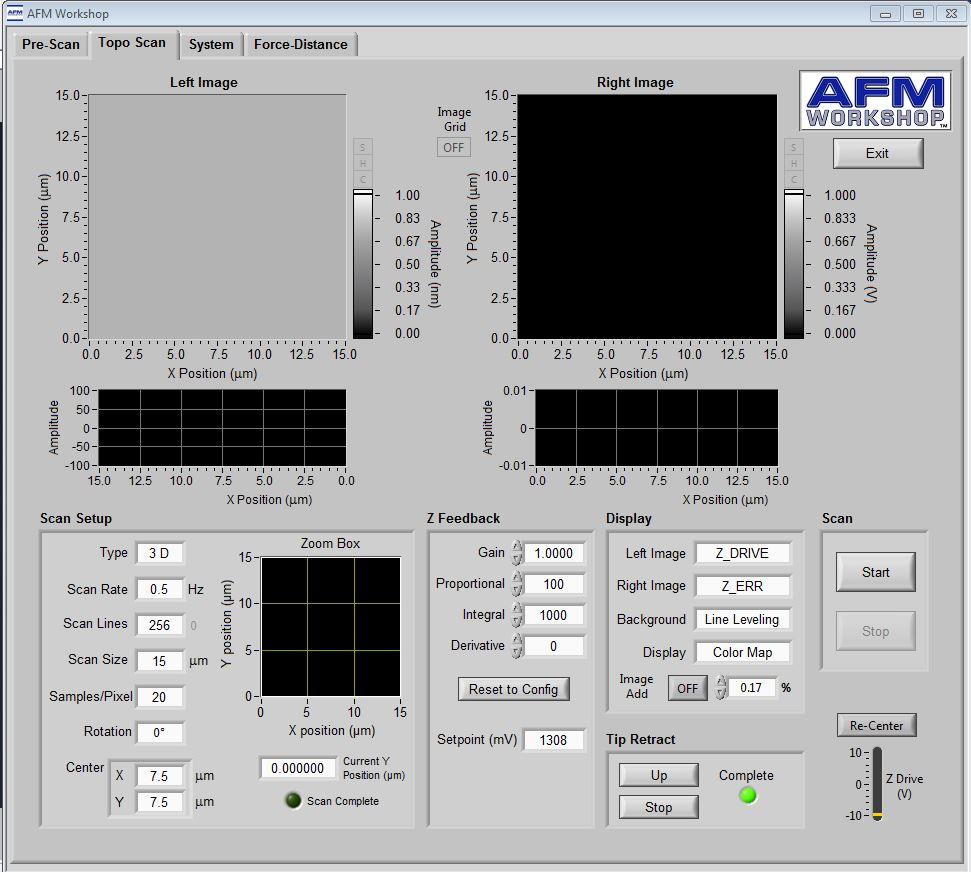
\includegraphics[width=0.45\linewidth]{images/toposcan.JPG}}
\end{center}

\begin{itemize}
    \item Scan Setup:

    \begin{itemize}
        \item Scan Rate - The number of lines per second scanned.

        \item Scan Size - The physical dimensions of the scan size. The highest this can go is 15 for the 15 micron scanner and 50 for the 50 micron scanner. A 15 micron scan will scan a 15 by 15 micron squared area.

        \item Scan Lines - The number of lines in the scan.

        \item Rotation - Either 0 or 90 degrees. At zero the scan will be build by scanning each line horizontally and at 90 degrees, each line is scanned vertically.

        \item Example: say you run a 15 micron scan with 256 lines at a rate of 1 Hz and rotation of 0 degrees. This will mean that the time it takes to scan one line \emph{horizontally} is 1 second. The speed at which the tip is moving horizontally is (15 $\mu$m) $\times$ (1 Hz) = 15 $\mu$m/sec.  The time it will take for the scan to complete is 256 seconds.
    \end{itemize}

    \begin{center}
        \href{http://experimentationlab.berkeley.edu/sites/default/files/AFMImages/scanningmethod.jpg}{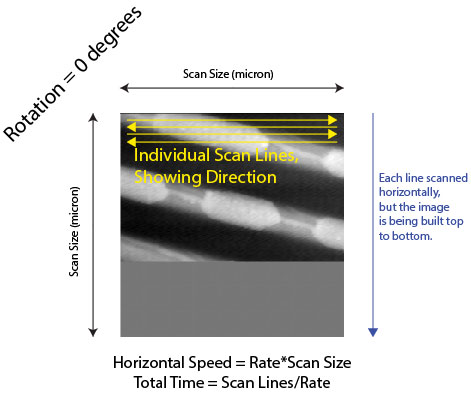
\includegraphics[width=0.6\linewidth]{images/scanningmethod.jpg}}
    \end{center}

    \item Z Feedback - Standard PID feedback loop.

    \begin{itemize}
        \item Integral - before doing a re-center in the pre-scan tab for automated tip approach, be sure to lower the integral value to 100, otherwise you \textbf{WILL} \hyperref[subsec:BrokenTip]{BREAK A TIP}. When the automated tip approach is complete, be sure to change the integral value back to 1000 before you start a scan.
    \end{itemize}

    \item Display

    \begin{itemize}
        \item Image Options (Left and Right Image) - The only options you should use are Z Drive, Z Error, and Phase. Z Drive gives height measurements. Z error gives the error in the feedback loop, meaning that rapid changes in topography will lead to sharp signals in the Z error measurement. Phase gives the phase change of oscillations in vibrating mode. Phase can be used to map surface hardness as the tip will get stuck in softer surfaces causing changes in phase. \textbf{DO NOT CHANGE THESE SETTINGS ONCE A SCAN HAS STARTED.}

        \item Background - Attempts to make each line flat. This is only for the display as you do the scan. The line leveling will not be recorded in the raw data. It is ok to change this setting once the scan has started.

        \item Image Add - Adds the right image on top of the left. Once again, this is only fo display purposes and will not be recorded in the data. It is ok to change this setting once the scan has started.

    \end{itemize}

\end{itemize}

\textbf{System Tab} - Where you will adjust parameters for resolution, minimizing error, and most importantly \textbf{NOT} \hyperref[subsec:BrokenTip]{BREAKING THE TIP}!

\begin{center}
    \href{http://experimentationlab.berkeley.edu/sites/default/files/AFMImages/systemtab.JPG}{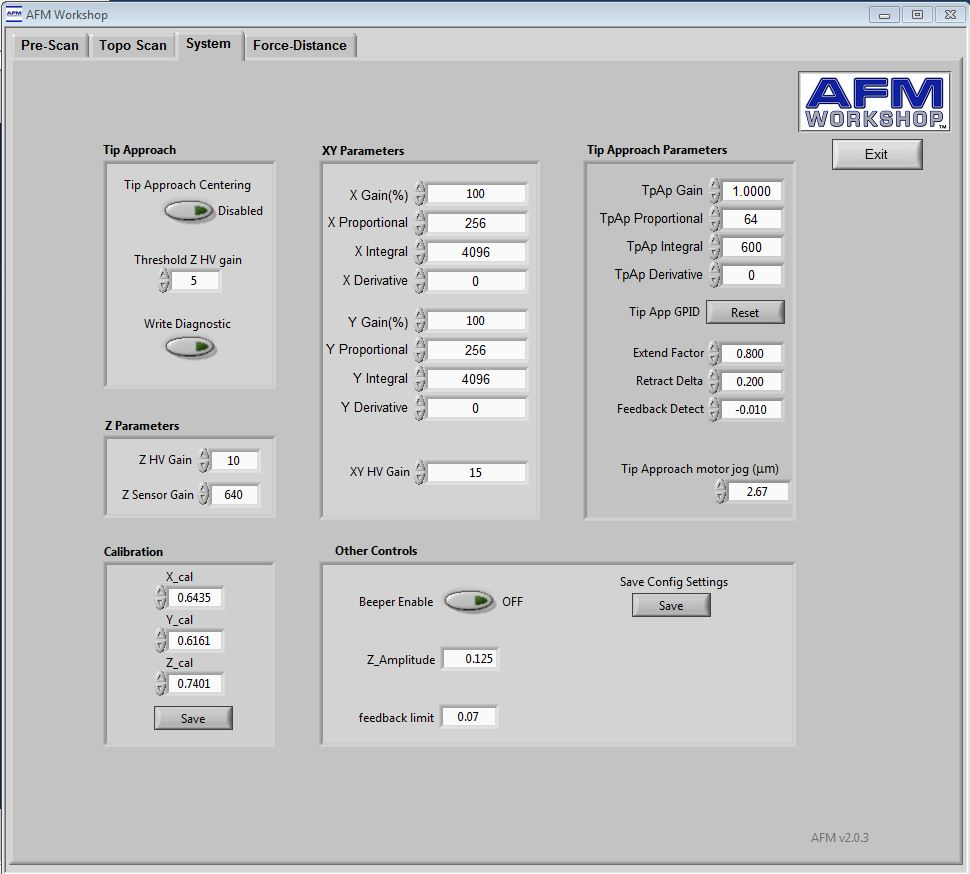
\includegraphics[width=0.5\linewidth]{images/systemtab.JPG}}
\end{center}

\begin{itemize}
    \item Z Parameters:

    \begin{itemize}
        \item The \emph{Z HV Gain} is set, depending on the Z Range of the the area of the sample being scanned.  A lower Z HV Gain theoretically results in a scan with less Z Noise, but also reduces the Z Range the scanner is capable of covering.  For all intents and purposes in this lab, you should only use a Z HV Gain between 5-10, because a tip approach with a Z HV Gain of less than 5 will result in a difficult tip approach, taking up to 30 minutes, and a scan with a Z HV Gain of greater than 10 will result in an image with less resolution and more noise.

        \item Refer to the \href{http://experimentationlab.berkeley.edu/tt-afmuserguidev2.2}{\textbf{TT-AFM User Guide}} pg.37 for a chart of the Theoretical resolution for each Z HV Gain value.

    \end{itemize}

    \item XY Parameters:

    \begin{itemize}
        \item Here are two standard GPID loops (see  \href{http://experimentationlab.berkeley.edu/sites/default/files/PID_Manual.pdf}{\textbf{PID Manual}} and \href{http://experimentationlab.berkeley.edu/sites/default/files/PID_Theory_Explained.pdf}{\textbf{PID Theory Explained}}), one for the X Piezo, and the other for the Y Piezo.  This controls the expansion characteristics of the XY piezos.

        \item The XY HV Gain controls how much the XY piezos are allowed to expand and contract.  This is set to 0 for noise floor scans, and 15 for all other functions.

    \end{itemize}

    \item Tip Approach Parameters:
    \begin{itemize}
        \item There is another standard GPID loop here that controls the tip approach.  The integral should never be raised above 800. Lower it by 50 if the tip has trouble engaging with the surface.  This will slow down the tip approach process.

        \item The \emph{Extend Factor} determines how much the the tip is lowered into the sample.  By default, its value is set at 0.800. In Vibrating mode, lowering this value will make the tip press into the sample MORE.  In non-Vibrating mode, lowering this value will make the tip press into the sample LESS.  In vibrating mode, if your tip approach has trouble properly engaging with the surface of the sample, decrease the extend factor by increments of 0.05 until it is properly zeroed.

        \item the \emph{Tip Approach Motor Jog} determines how much the tip is lowered to the sample's surface with each increment during the Automated Tip Approach.  Lowering the Z HV Gain, under Z Parameters, will lower the maximum allowed Tip Approach Motor Jog size.
    \end{itemize}

    \item Calibration:
    \begin{itemize}
        \item XYZ Calibration values are set by scanning a sample with known dimensions, such as a reference slide, and then inputting the measured and actual values into a program to calculate the Calibration values to ensure that the scanner for the AFM returns accurate values. Multiple calibrations may be required to increase the precision of your AFM. You will be expected to scan the reference slide and perform your own system calibration in this lab.
    \end{itemize}

\end{itemize}

\pagebreak

\section{Experimental Procedure}

As you follow along with the lab write up, you will find the following instructional videos to be \textbf{VERY USEFUL}. Watch them in order as you go through the lab write up (they are located below in specific sections as well):

\begin{itemize}
    \item \href{http://experimentationlab.berkeley.edu/sites/default/files/gettingstarted\_final2.mp4}{\textbf{Getting Started and Probe Exchange}},

    \item \href{http://experimentationlab.berkeley.edu/sites/default/files/alignment\_final2.mp4}{\textbf{Alignment: Camera, Laser, and Detector}}, and

    \item \href{http://experimentationlab.berkeley.edu/sites/default/files/prescan\_final2.mp4}{\textbf{Pre-Scan: Tune Frequency, Tip Approach, and Scanning}}
\end{itemize}

These instructional videos are referenced in the procedures below.

\subsection{Turn on instruments and open programs}
\label{subsec:TurnOnInstrumentsAndOpenPrograms}

For this section, refer to information in the instructional video  \href{http://experimentationlab.berkeley.edu/sites/default/files/gettingstarted\_final2.mp4}{\textbf{Getting Started and Probe Exchange}}

\begin{itemize}
    \item Power on the Ebox via the switch in the lower rear
    \begin{itemize}
        \item Series of green LED lights will illuminate when power is on
    \end{itemize}
    \begin{center}
    \href{http://experimentationlab.berkeley.edu/sites/default/files/EBOX2.jpg}{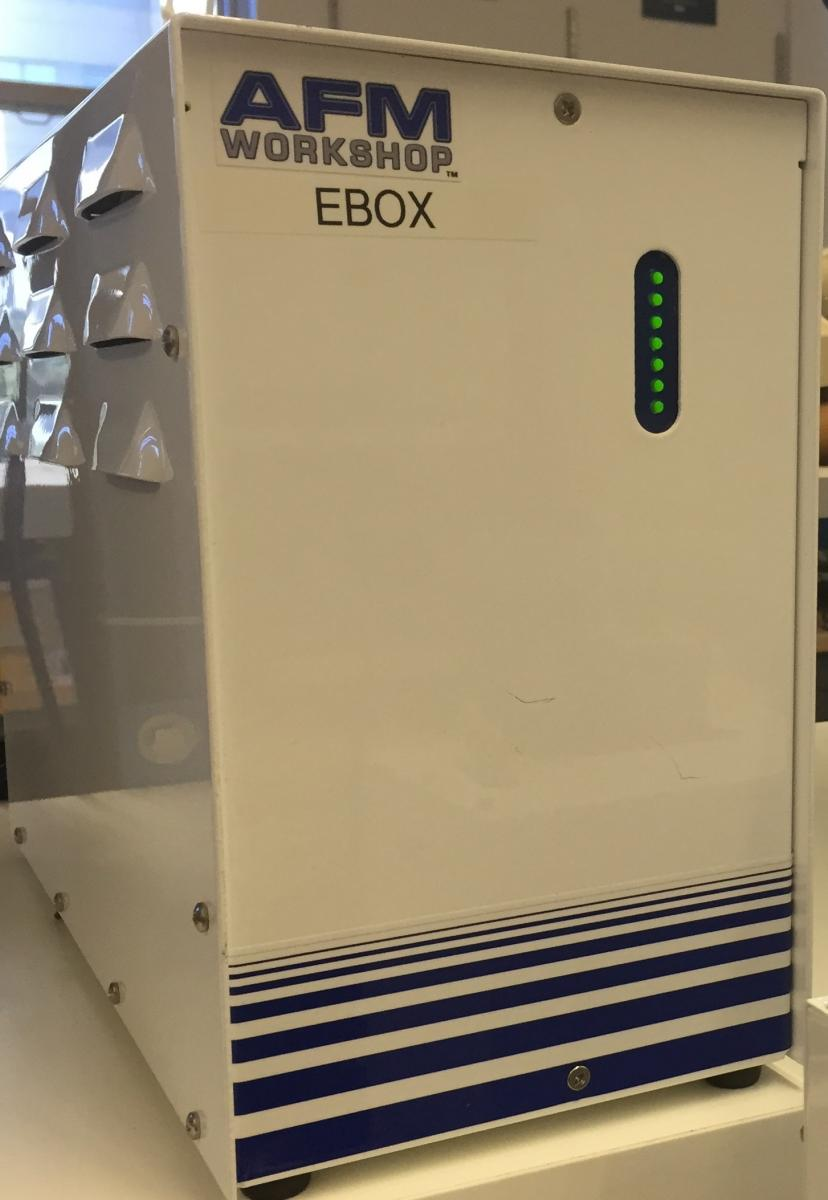
\includegraphics[width=0.33\linewidth,keepaspectratio]{images/EBOX2.jpg}}
    \href{http://experimentationlab.berkeley.edu/sites/default/files/AFMImages/10.JPG}{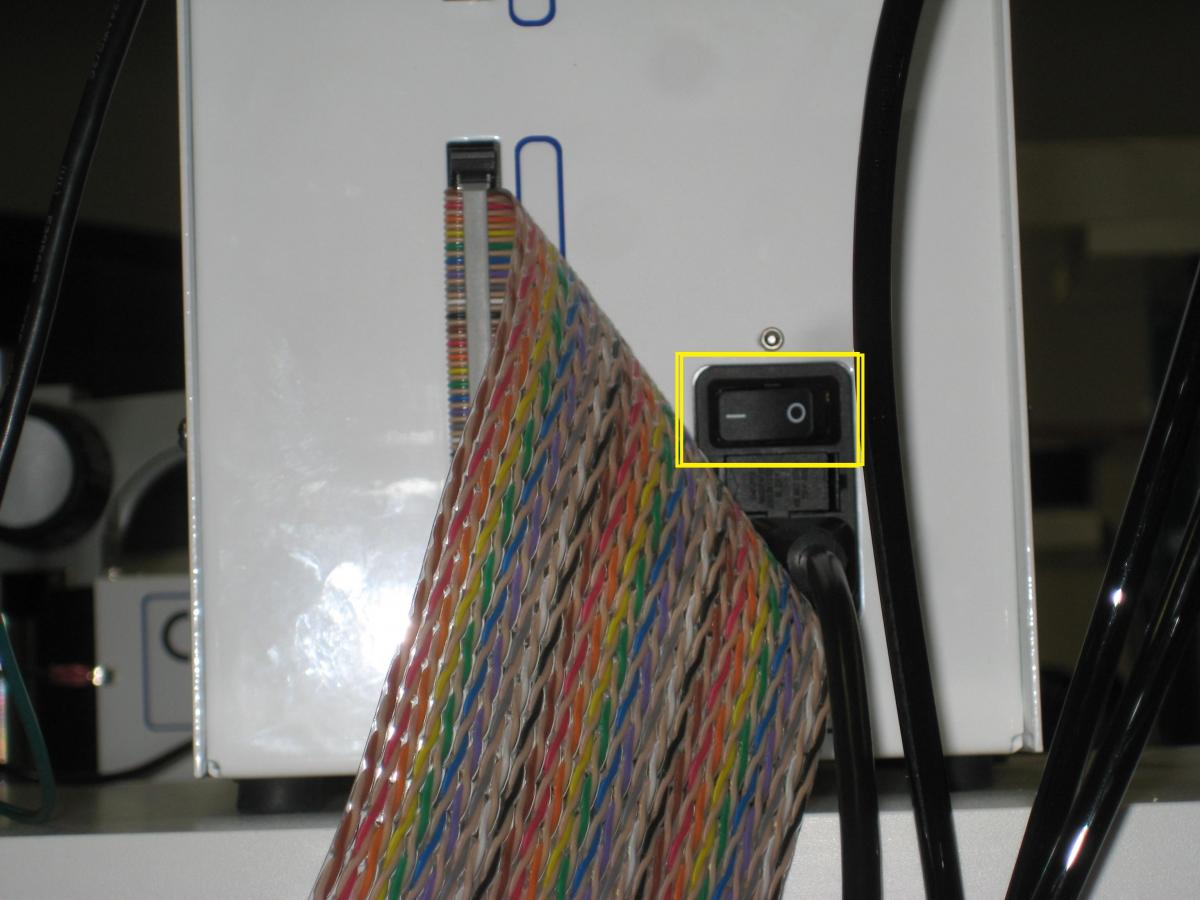
\includegraphics[width=0.33\linewidth,keepaspectratio]{images/10.JPG}}
    \\Ebox
    \end{center}

    \item Turn on LED illuminator
    \begin{center}
    \href{http://experimentationlab.berkeley.edu/sites/default/files/AFMImages/LED1.jpg}{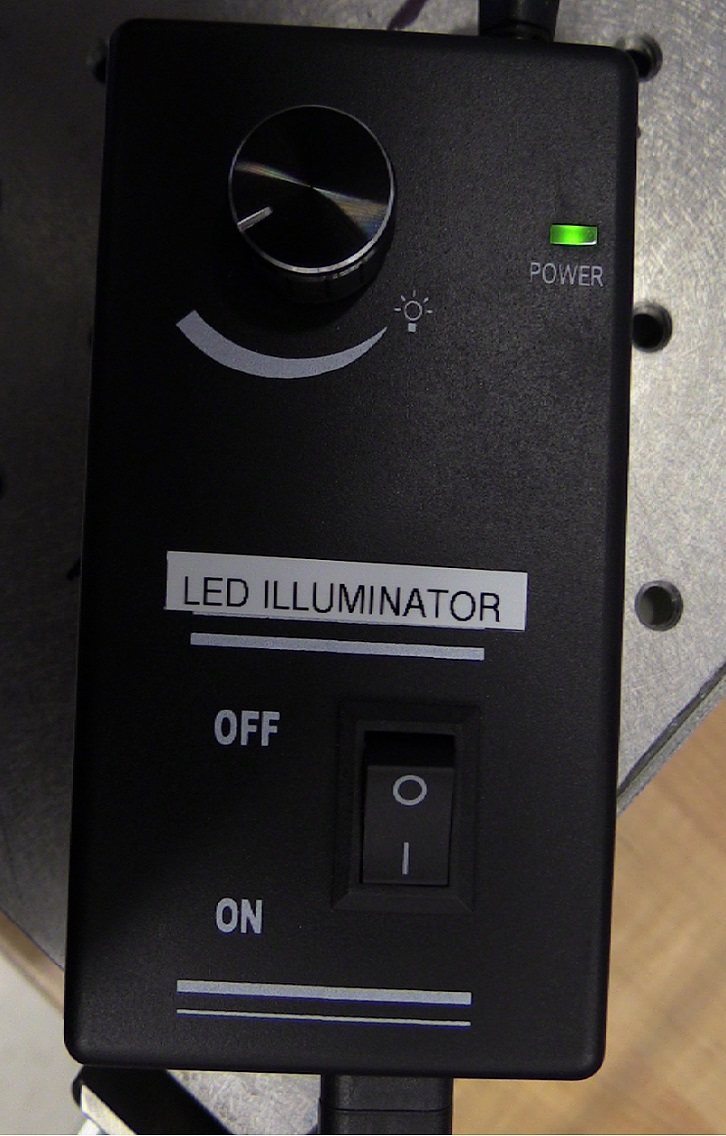
\includegraphics[width=0.33\linewidth,keepaspectratio]{images/LED1.jpg}}
    \href{http://experimentationlab.berkeley.edu/sites/default/files/AFMImages/LED2.jpg}{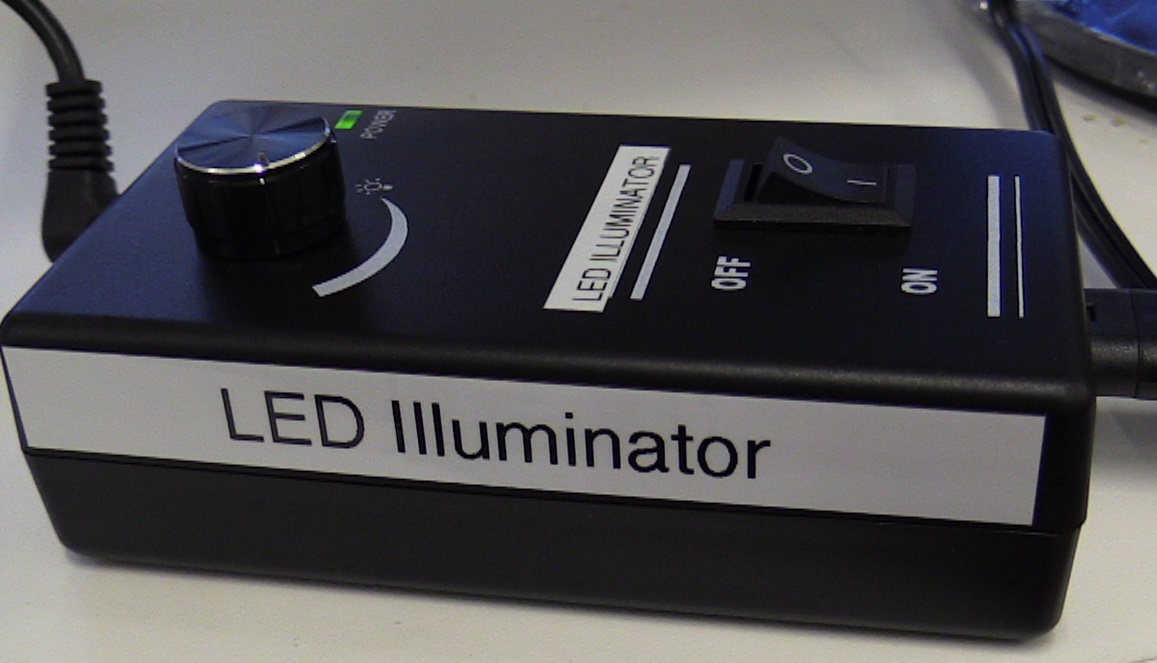
\includegraphics[width=0.33\linewidth,keepaspectratio]{images/LED2.jpg}}
    \end{center}

    \item Make sure the grounding plug is plugged in, which is located on the back of the AFM.  The grounding plug is the silver plug outlined by the yellow rectangle shown in the figure below.  **Note that in the figure below the grounding plug is already plugged in.  It should already be plugged in because the stage needs to be grounded. The only reason it would ever need to be unplugged is if you wanted to use the Conductive Mode of AFM, which we will NOT be using in this lab.
    \begin{center}
    \href{http://experimentationlab.berkeley.edu/sites/default/files/AFMImages/12.JPG}{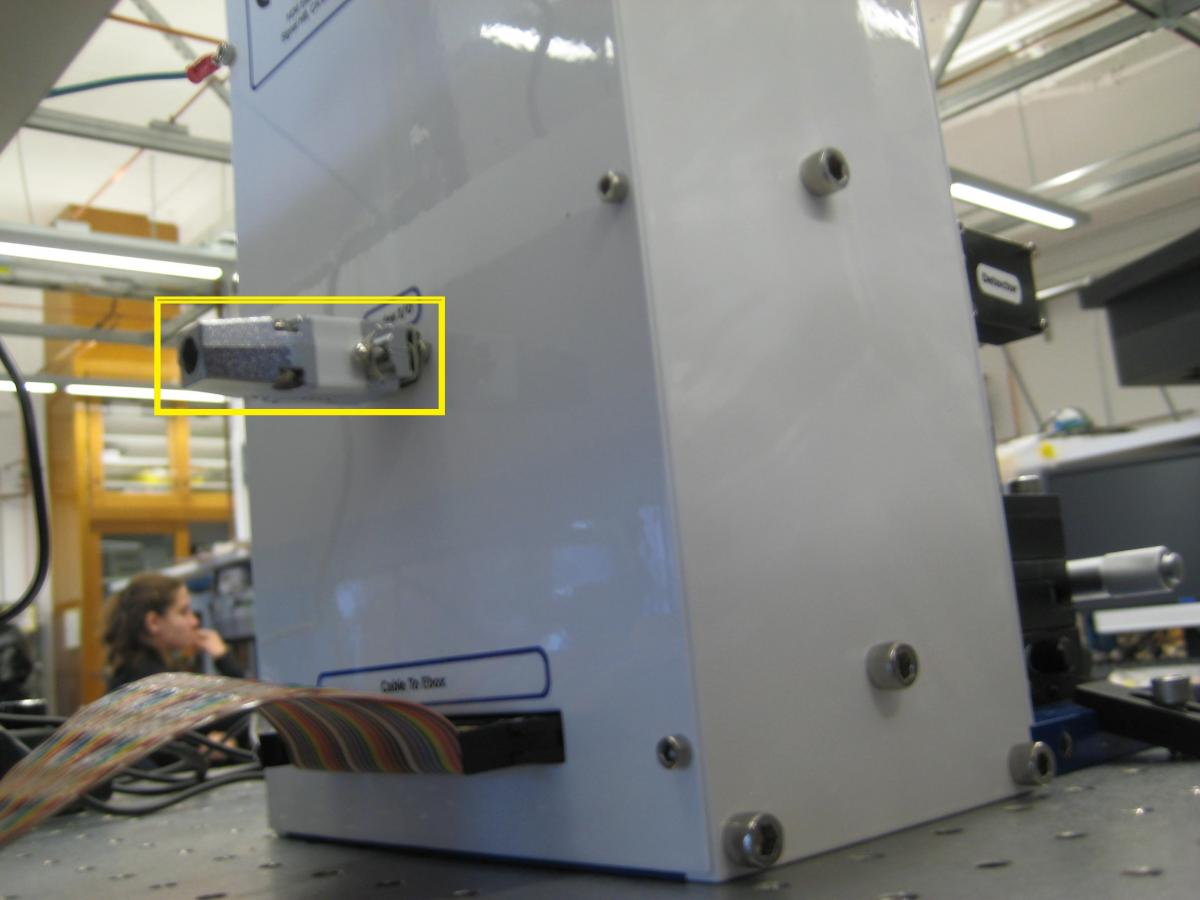
\includegraphics[width=0.5\linewidth]{images/12.JPG}}
    \end{center}

    \item In C:/AFM Experiment, double click and open
    \begin{itemize}
        \item 2.0.3-15 Micron Shortcut for the 15 micron scanner

        \item AFM Workshop 2.4.15 shortcut for the 50 micron scanner

        \item USB2.0-Camera (click the play button on the top left of the program window to start the camera)

        \begin{itemize}
            \item \textbf{Remove the lens cap from the camera }(bottom of black camera tube)

        \end{itemize}

    \end{itemize}

    \item \textbf{NOTE:} If you are experiencing bugs, please refer to the \hyperref[sec:Troubleshooting]{troubleshooting section} at the end of this lab

\end{itemize}

Before you start each day (and after changing out scanners), make sure you have control over the instrument. Do this after turning everything on. Go to the \textbf{Manual Z Motor Control} in the \textbf{Pre Scan} tab of the software and click \textbf{UP} to ensure that the z motor moves the probe upward.  When you are moving the Z motor UP you should be able to hear the motor and physically see the probe moving up and away from the sample. If it doesn't move then close the software and launch it again.

\begin{itemize}
    \item You must always be careful you \textbf{DO NOT} click on the DOWN button BEFORE making sure that the probe tip is not anywhere close to the sample, and that you have reduced the speed on the slider bar to a very low value so you do not \hyperref[subsec:BrokenTip]{crash the tip}.
\end{itemize}

\subsection{Removing/Installing Probes} (PROCEED WITH CAUTION -- THE PROBES ARE VERY DELICATE)

\begin{enumerate}
    \item \textbf{NEVER PICK UP THE PROBE WITH YOUR HANDS, THIS WILL CONTAMINATE AND \hyperref[subsec:BrokenTip]{DESTROY THE TIP}}

    \item \textbf{NEVER PICK UP THE PROBE ALONG THE LONG LENGTH, THIS WILL \hyperref[subsec:BrokenTip]{DESTROY THE TIP}}

    \item \textbf{NEVER INTERACT WITH THE TIP OF THE PROBE WHILE PERFORMING A PROBE EXCHANGE, THIS WILL \hyperref[subsec:BrokenTip]{DESTROY THE TIP}}
\end{enumerate}

Follow the steps below to remove the probe holder from the AFM to install a probe into the probe holder, or if you need to replace the probe for which ever reason (i.e. broken tip, damaged tip, no tip mounted in tip holder, etc.)

Watch this quick \href{http://experimentationlab.berkeley.edu/sites/default/files/AFMImages/2.0ProbeExchange\_Ver1.1.wmv}{\textbf{video tutorial}} (which can also be found on the experimentation lab computers in C:/AFM Experiment/Instructional Videos/2.0ProbeExchange\_Ver1.1.wmv) and this other tutorial \href{http://experimentationlab.berkeley.edu/sites/default/files/gettingstarted\_final2.mp4}{\textbf{Getting Started and Probe Exchange}} for information on replacing a probe \textbf{IN ADDITION TO} reading the more detailed written steps below.

Watching the video and following along will ultimately save you time.

\begin{enumerate}
    \item On the TT-AFM, turn the z micrometer adjustment knob (labeled ``Z Control'', located behind the camera tube on top of the AFM) clockwise to raise the tip a reasonable distance ($\sim$2cm) away from the sample holder to avoid accidentally bumping into anything when removing the tip holder from the apparatus.

    \begin{figure}[H]
        \centering
        \href{http://experimentationlab.berkeley.edu/sites/default/files/AFMImages/AFMstagespace_0.jpg}{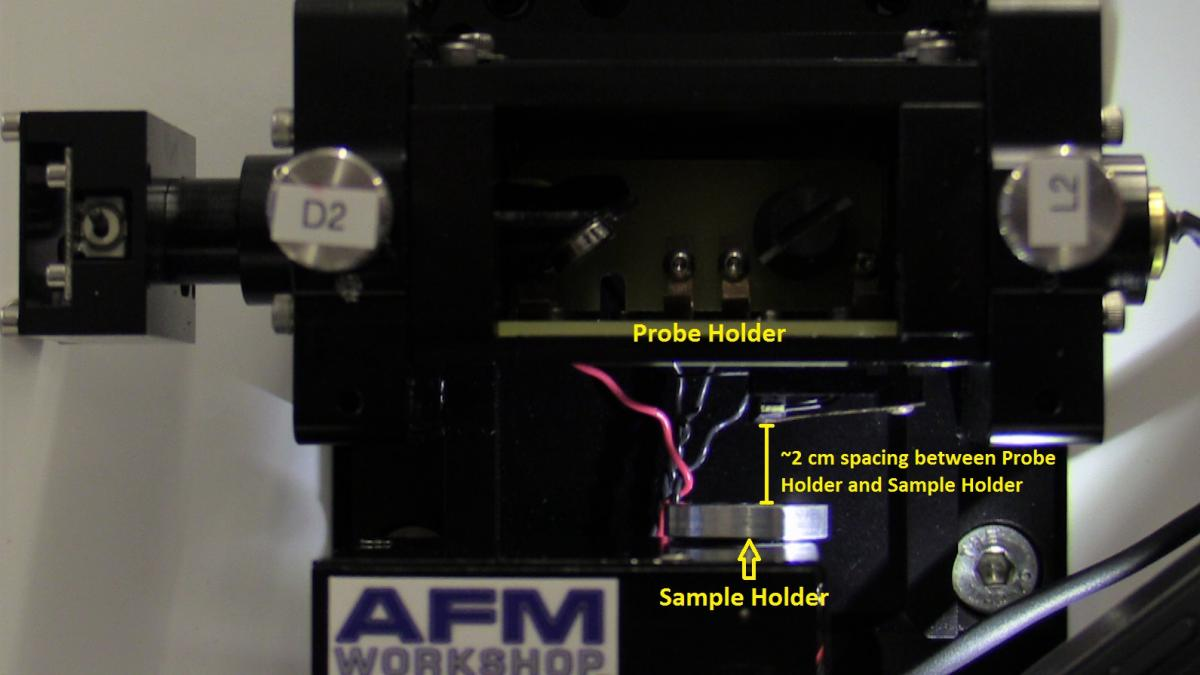
\includegraphics[width=0.9\linewidth]{images/AFMstagespace_0.jpg}}
        \caption{Proper spacing between probe holder and sample holder}
        \label{fig:AFMStageSpace}
    \end{figure}
    
    \item Only after you have made sure that there is a large distance between the probe holder (the yellow slide in Figures \ref{fig:AFMStageSpace} and \ref{fig:PullOutYellowSlide}) and the sample holder (the metallic disk on the stage in Figure~\ref{fig:AFMStageSpace}), you can remove the probe holder by gripping and pulling the black tab/handle.

    \begin{figure}[H]
        \centering
        \href{http://experimentationlab.berkeley.edu/sites/default/files/AFMImages/14.JPG}{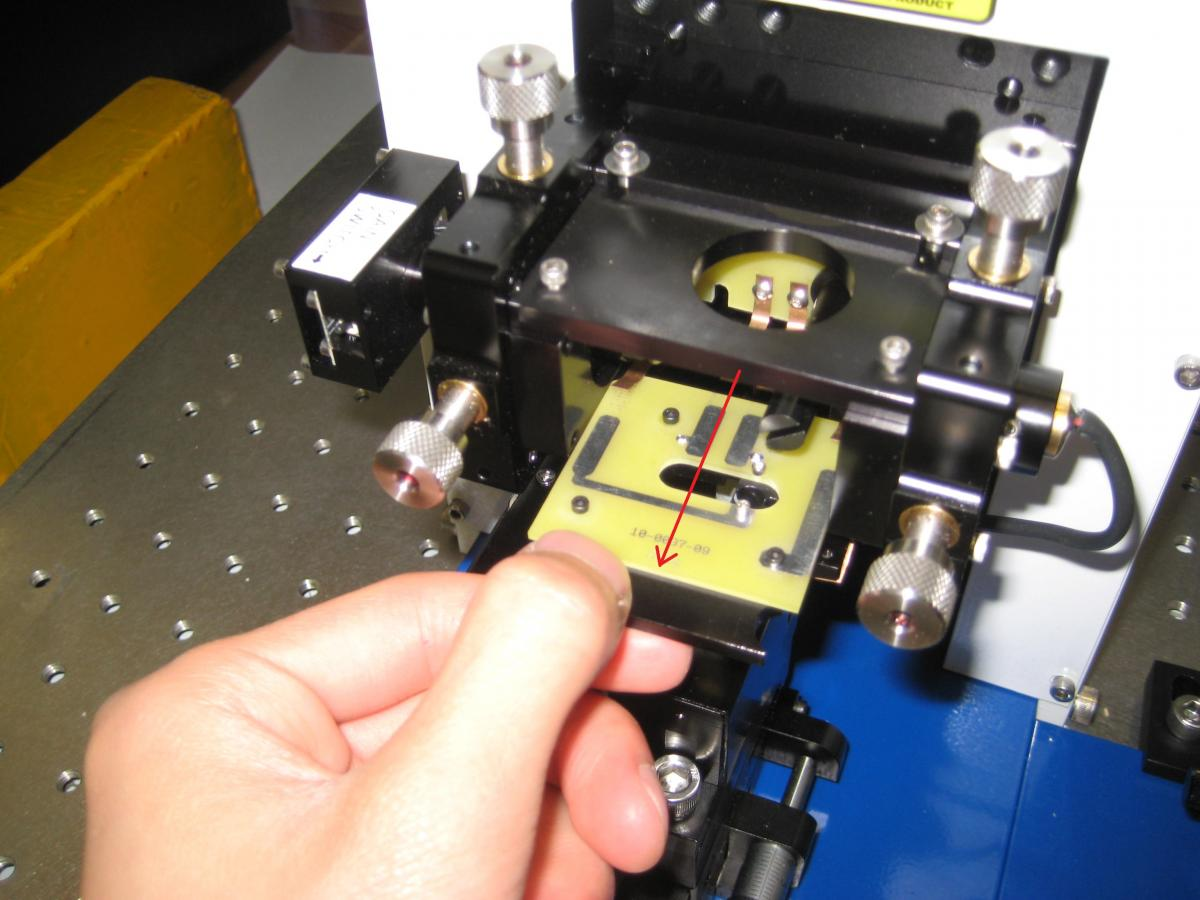
\includegraphics[width=0.6\linewidth]{images/14.JPG}}
        \caption{Removing the probe holder}
        \label{fig:PullOutYellowSlide}
    \end{figure}

    \item Once the probe holder is removed from the TT-AFM, flip the holder over so that the \textbf{copper probe clip is face up}. Gently place the probe holder down in a clean, open, workspace with the \textbf{copper probe clip face up}. If there is already a working probe installed in the probe holder, \hyperref[subsec:HowToPrepareASample]{you may skip this step}.  If you have damaged the probe and need to replace it, or are installing a new probe, proceed with the instructions below.

    \begin{figure}[H]
        \centering
        \href{http://experimentationlab.berkeley.edu/sites/default/files/AFMImages/15.JPG}{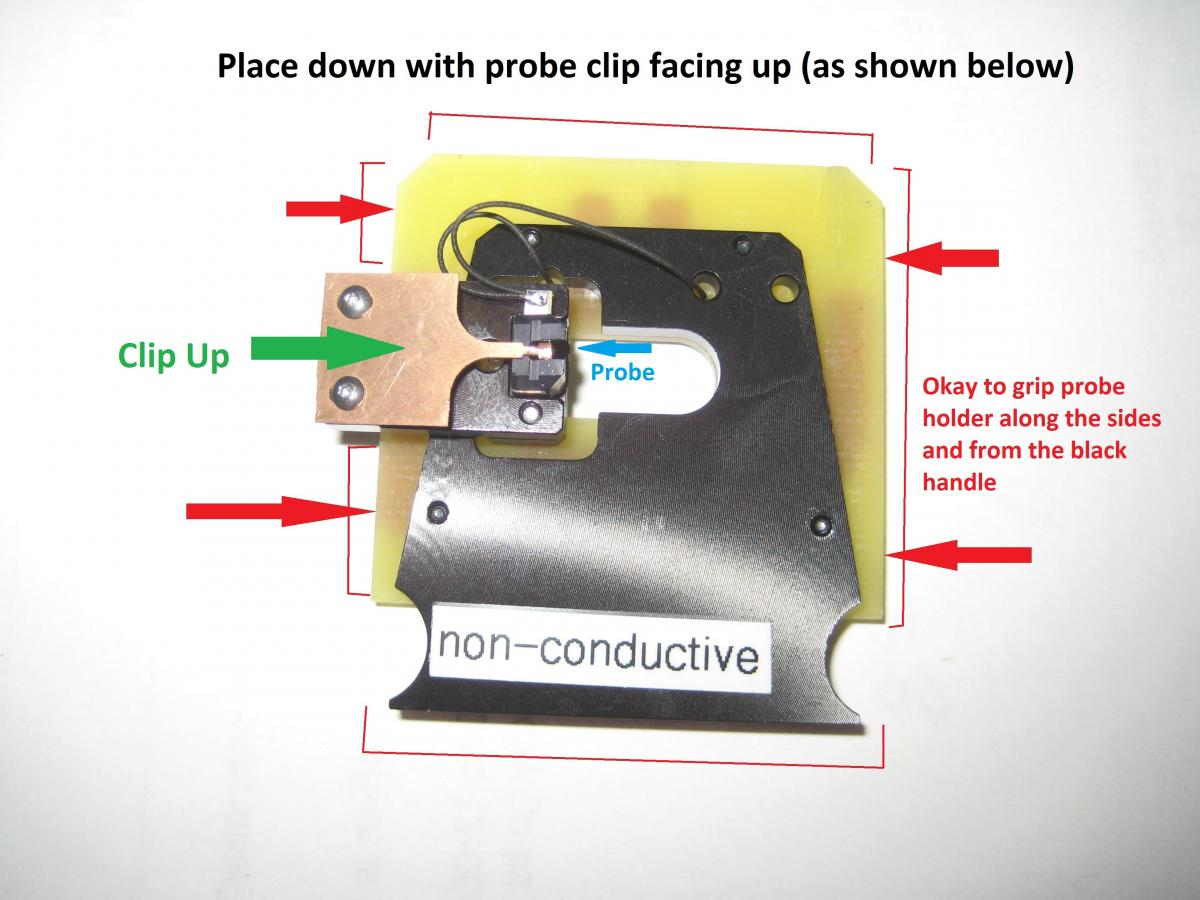
\includegraphics[width=0.6\linewidth]{images/15.JPG}}
        \caption{}
        \label{fig:YellowSlideDescription}
    \end{figure}
    
    \item Locate the appropriate exchange tool, \textbf{identifiable by their matching labels.} We have two exchange tools (the two black rectangles below the two probe holders in Figure~\ref{fig:ProbeHolderExchange}), one for the non-conductive probe holder and one for the conductive probe holder. In this lab we will be using on the Non-Conducting Probe Holder and Non-Conducting Exchange tool.
    \begin{enumerate}
        \item **IT IS VERY IMPORTANT TO ONLY USE THE NON-CONDUCTIVE PROBE HOLDER WITH THE NON-CONDUCTING EXCHANGE TOOL.  Placing the probe holder on the wrong exchange tool may result in a \hyperref[subsec:BrokenTip]{broken tip}!**

        \item For this lab, we will be using the \textbf{NON-CONDUCTIVE probe holder} and the \textbf{NON-CONDUCTIVE exchange tool.}
    \end{enumerate}

    \begin{figure}[H]
        \centering
        \href{http://experimentationlab.berkeley.edu/sites/default/files/AFMImages/ProbeHolderExchange.png}{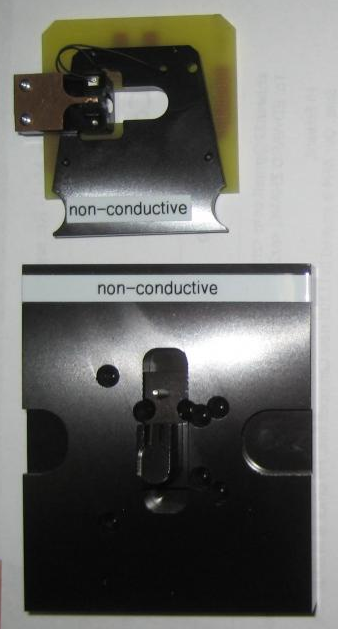
\includegraphics[width=0.35\linewidth]{images/ProbeHolderExchange.png}}
        \caption{Non-conductive probe holder and exchange tool}
        \label{fig:ProbeHolderExchange}
    \end{figure}
    
    \item Pick up your probe holder appropriately (areas okay to grip are labeled in Figure~\ref{fig:YellowSlideDescription} in step 3), then \textbf{carefully and gently} lower the probe holder on to its matching exchange tool.  The bolt will go into the smaller hole directly under the narrow part of the copper clip, and the larger oval structure on the exchange tool will go through the large oval hole in the probe holder, shown in the image below.
    \begin{enumerate}
        \item Notice how the labels are relative to each other in the image below.

        \item The probe holder should \textbf{sit flush} on the exchange tool
    \end{enumerate}

    \begin{figure}[H]
        \centering
        \href{http://experimentationlab.berkeley.edu/sites/default/files/AFMImages/17.JPG}{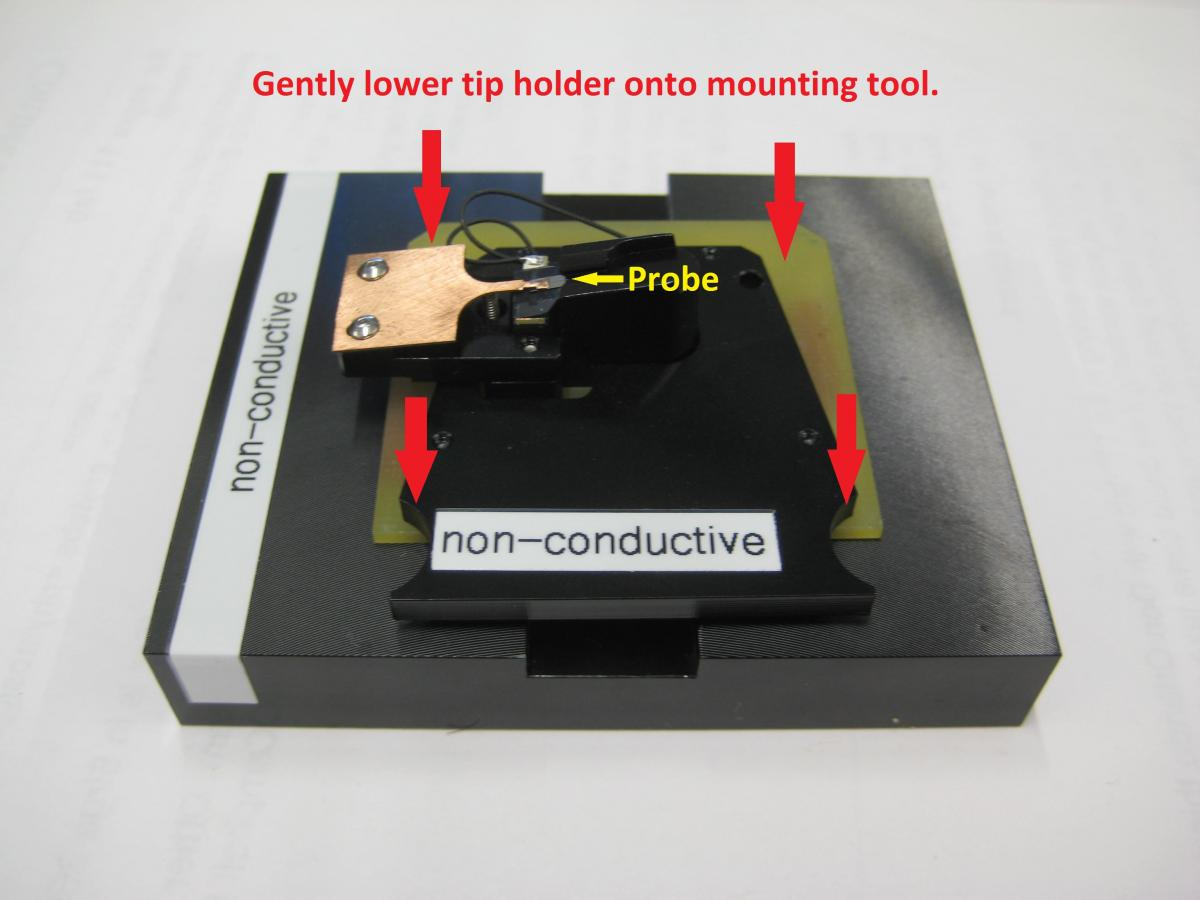
\includegraphics[width=0.55\linewidth]{images/17.JPG}}
        \caption{}
    \end{figure}
    
    \item If you are \textbf{removing a broken probe}, proceed with these next steps (step 6 and step 7). If you are\textbf{ installing a new probe, skip to step 9}. \textbf{Firmly grip the probe holder and the exchange tool together} (pressing down causes the bolt on the exchange tool to push up on the probe clip on the probe holder, releasing the probe).  With the label on the exchange tool closest to you (text will be upside down, refer to Figure~\ref{fig:HoldingTool}), tilt it slightly forward ($\sim$10 degrees) and \textbf{gently tap it on the table to cause the probe to slide out of the clip} and into the oval ``cup'' of the exchange tool.
    \begin{itemize}
        \item It is \textbf{highly recommended} to refer to the tutorial video \href{http://experimentationlab.berkeley.edu/sites/default/files/gettingstarted\_final2.mp4}{\textbf{Getting Started and Probe Exchange}}.
    \end{itemize}

    \begin{figure}[H]
        \centering
        \href{http://experimentationlab.berkeley.edu/sites/default/files/AFMImages/18.JPG}{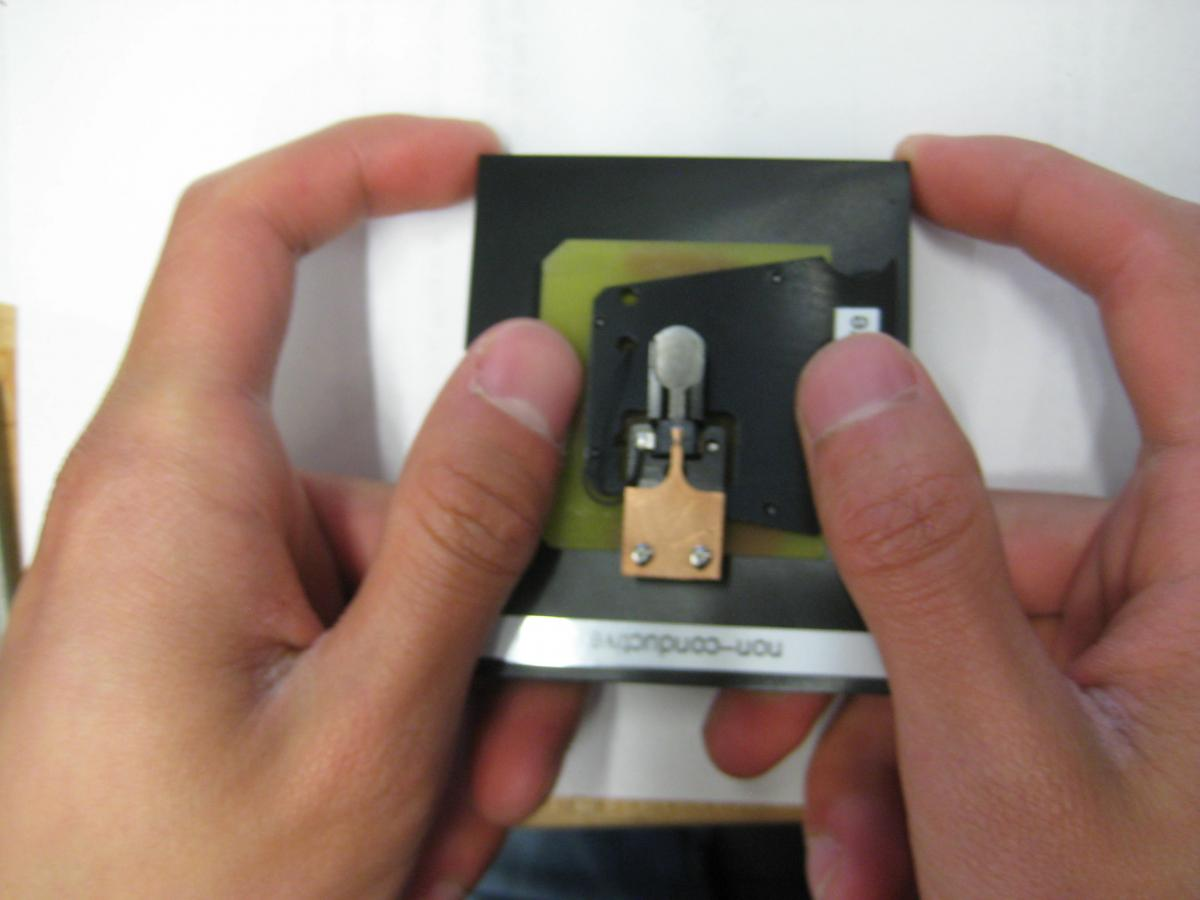
\includegraphics[width=0.5\linewidth]{images/18.JPG}}
        \caption{}
        \label{fig:HoldingTool}
    \end{figure}
    
    \begin{figure}[H]
        \centering
        \href{http://experimentationlab.berkeley.edu/sites/default/files/AFMImages/19.JPG}{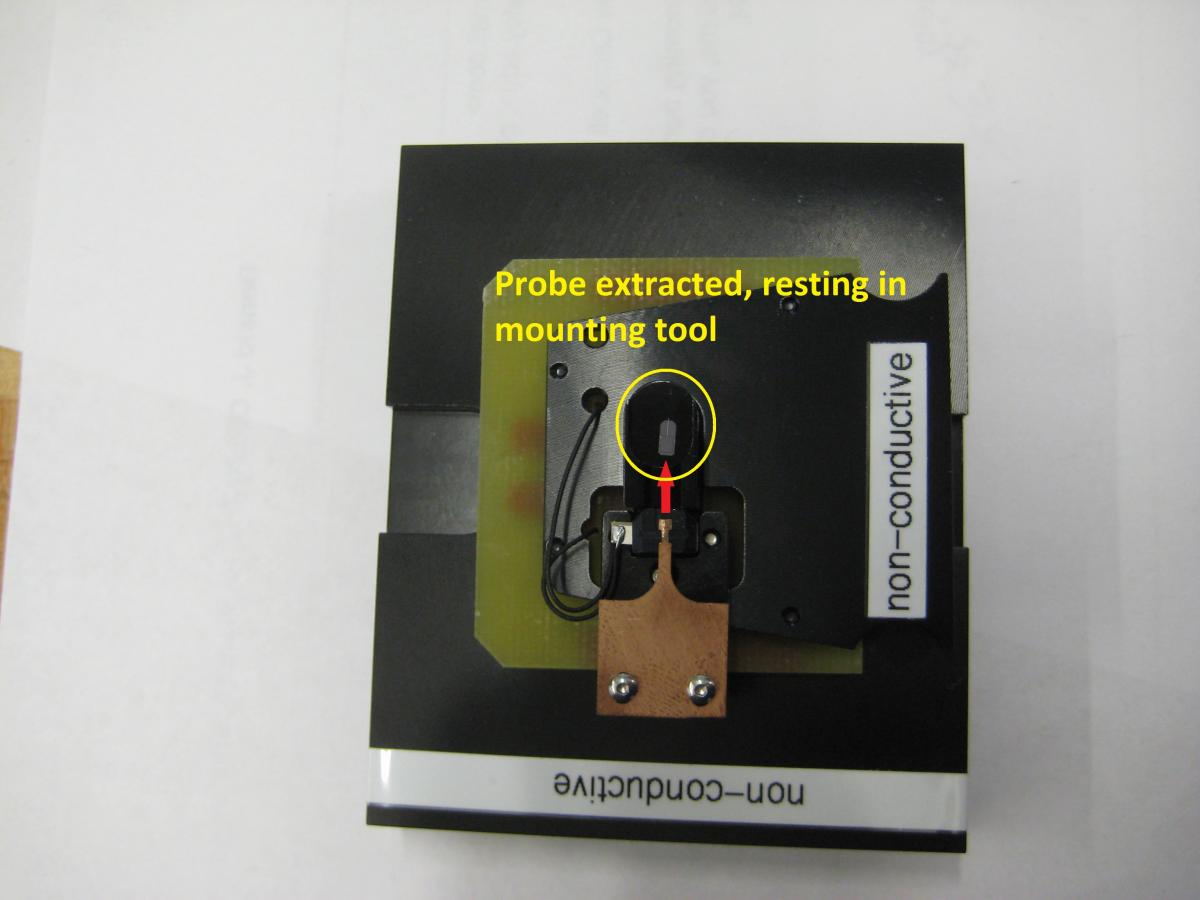
\includegraphics[width=0.5\linewidth]{images/19.JPG}}
        \caption{}
    \end{figure}
    
    \item Using fine tipped tweezers, pick up the probe by \textbf{pinching it by the narrow length}, and place it into the gel bed probe case.
    \begin{itemize}
        \item \textbf{NEVER PICK UP THE PROBE WITH YOUR HANDS, THIS WILL CONTAMINATE AND \hyperref[subsec:BrokenTip]{DESTROY THE TIP}}

        \item \textbf{NEVER PICK UP THE PROBE ALONG THE LONG LENGTH, THIS WILL \hyperref[subsec:BrokenTip]{DESTROY THE TIP}}

        \item \textbf{NEVER INTERACT WITH THE TIP OF THE PROBE WHILE PERFORMING A PROBE EXCHANGE, THIS WILL \hyperref[subsec:BrokenTip]{DESTROY THE TIP}}
    \end{itemize}

    \begin{figure}[H]
        \centering
        \href{http://experimentationlab.berkeley.edu/sites/default/files/AFMImages/20.JPG}{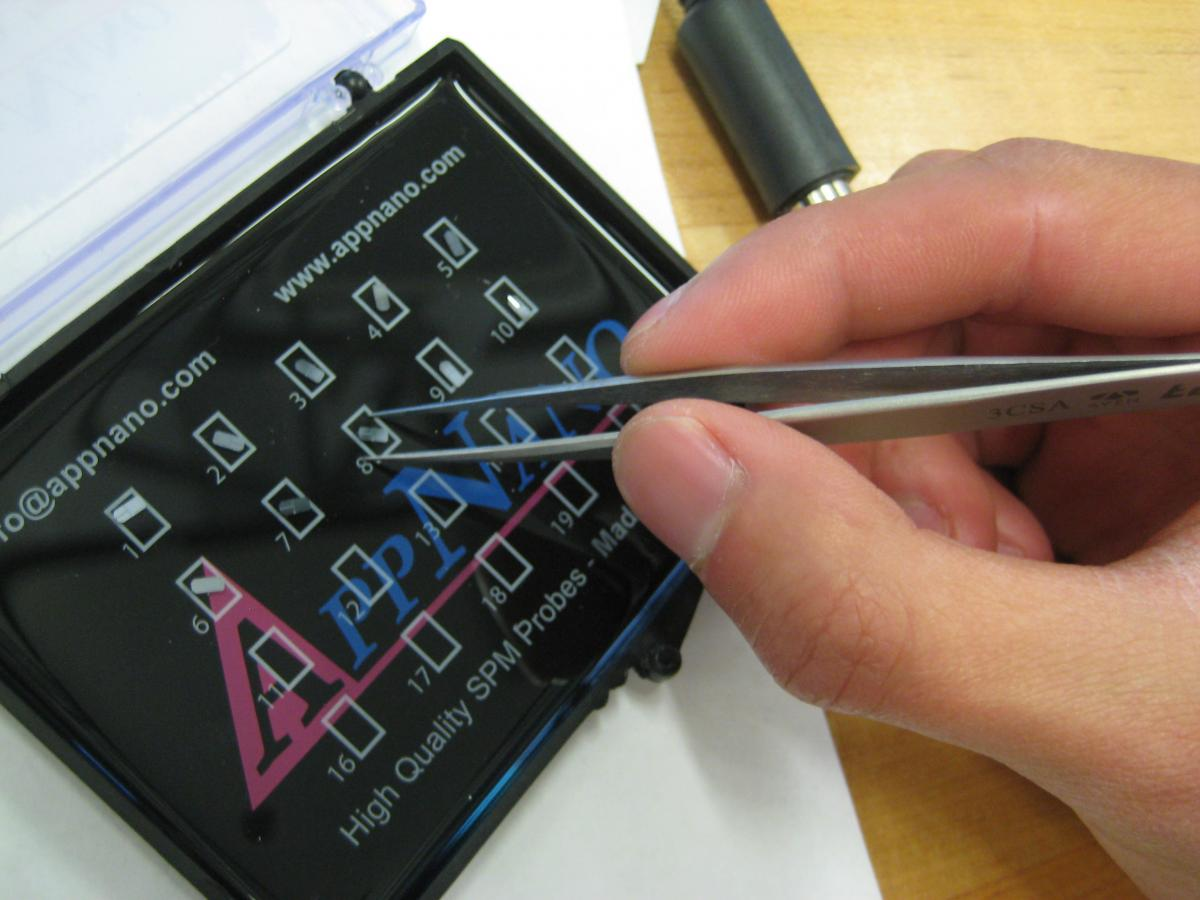
\includegraphics[width=0.5\linewidth]{images/20.JPG}}
        \caption{}
        \label{fig:ProbeBox}
    \end{figure}
    
    \item If you are switching from non-conductive mode to conductive mode or vice versa \textbf{(NOTE: we will NOT be using conductive mode in this lab)}:
    \begin{itemize}
        \item remove the currently mounted probe holder from its exchange tool, as to not wear out the clip on the probe holder, and set it aside.

        \item Grab the correct probe holder that you plan on using next, and mount it on the \textbf{correct} exchange tool.
    \end{itemize}
    
    \item \textbf{INSTALLING A NEW PROBE:}  Open the box containing the probes \textbf{very carefully} (shown in Figure~\ref{fig:ProbeBox}).
    
    \begin{itemize}
        \item \textbf{BEFORE you pick up the probe, note which side of the probe has the cantilever and tip as shown in the image below.}  The probe should be oriented this way when you pick it up using the finely tipped tweezers labeled ``Probe Use Only.''
    
        \begin{center}
            \href{http://experimentationlab.berkeley.edu/sites/default/files/AFMImages/AFMprobe.JPG}{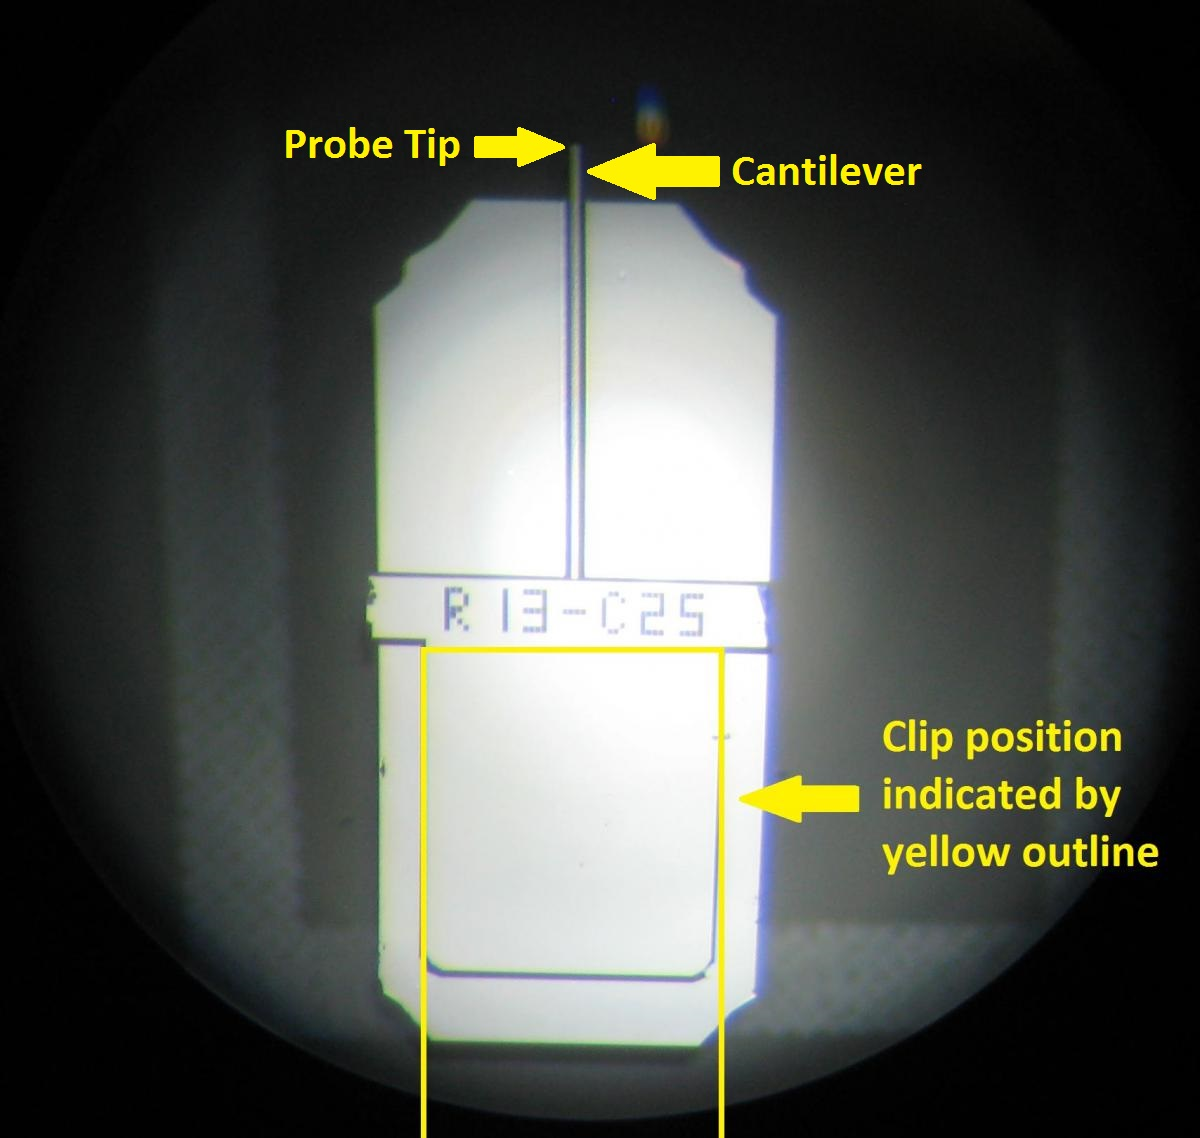
\includegraphics[width=0.5\linewidth]{images/AFMprobe.JPG}}
        \end{center}
    
        \item Using the finely tipped tweezers labeled ``Probe Use Only'', \textbf{slowly and with great care}, pick up a new probe along the narrow length.
    
        \item With the tip of the new probe oriented \textbf{AWAY FROM} the copper probe clip on the probe holder, \textbf{GENTLY} place the new probe in the oval on the exchange tool (Figure~\ref{fig:ExchangeTool}).
    \end{itemize}
    
    \begin{figure}[H]
        \centering
        \href{http://experimentationlab.berkeley.edu/sites/default/files/AFMImages/21.JPG}{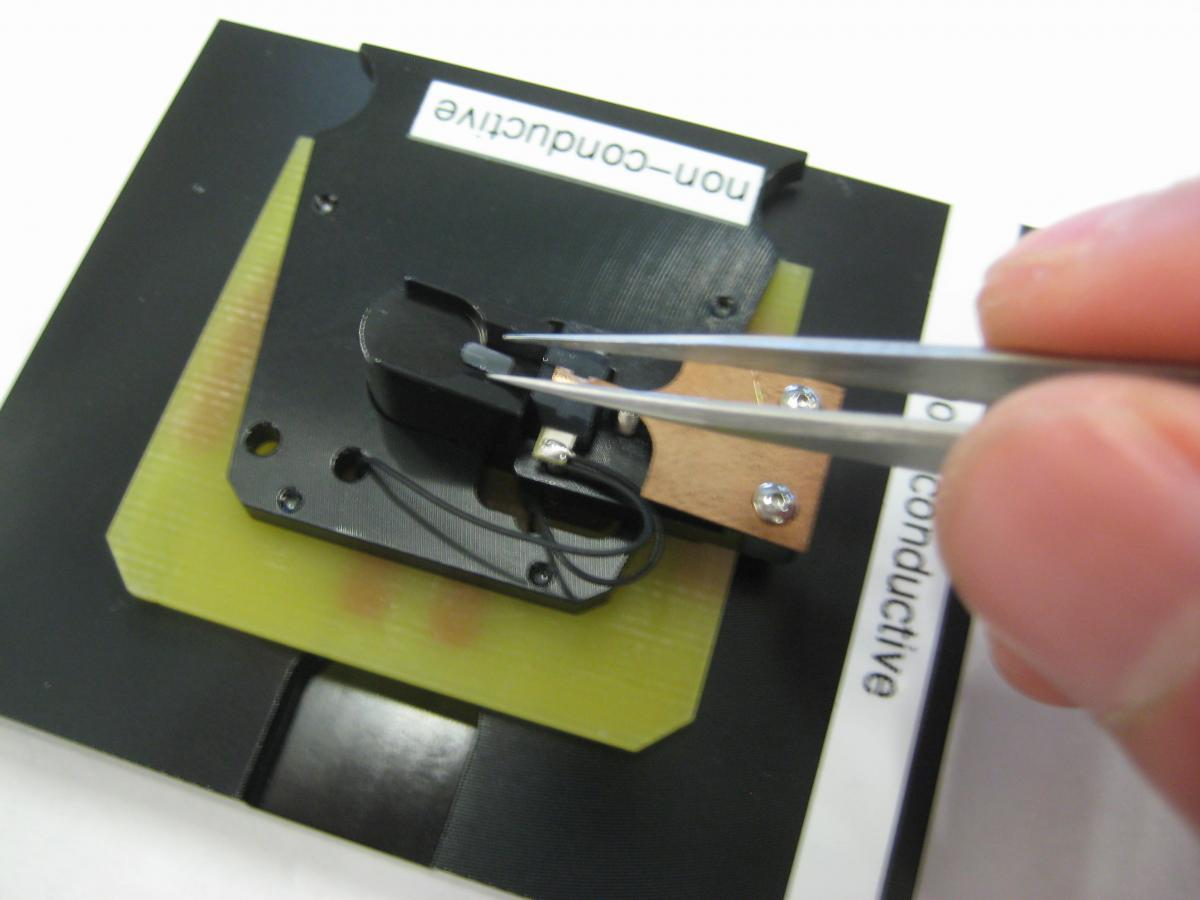
\includegraphics[width=0.5\linewidth]{images/21.JPG}}
        \caption{}
        \label{fig:ExchangeTool}
    \end{figure}
    
    \item  Grip the probe holder with the exchange tool, slightly tilting them towards yourself ($\sim$10 degrees), and tap it gently it on the table until the probe slides down the track and under the clip.
    
    \begin{itemize}
        \item \textbf{DO NOT TILT THE TOOL TOO FAR BACK, BECAUSE THIS WILL CAUSE THE PROBE TO SLIDE BACK TOO FAST AND SLIDE PAST THE CLIP AND FALL INTO THE CREVICE BEHIND IT, POSSIBLY DAMAGING THE PROBE.}
        \begin{itemize}
            \item \textbf{If this happens, DO NOT release the clip. Tilt it the other way and see if you can get the probe to slide back out.  If this is not possible, see if you can gently shake the probe out of the side and on to a piece of paper. Then pick up the probe with tweezers and try again, more carefully this time.}
        \end{itemize}
    
        \item Recommended to watch tutorial video \href{http://experimentationlab.berkeley.edu/sites/default/files/gettingstarted\_final2.mp4}{\textbf{Getting Started and Probe}}\href{http://experimentationlab.berkeley.edu/sites/default/files/gettingstarted\_final2.mp4}{\textbf{Exchange}} for this step
    \end{itemize}
    
    \begin{figure}[H]
        \centering
        \href{http://experimentationlab.berkeley.edu/sites/default/files/AFMImages/22.JPG}{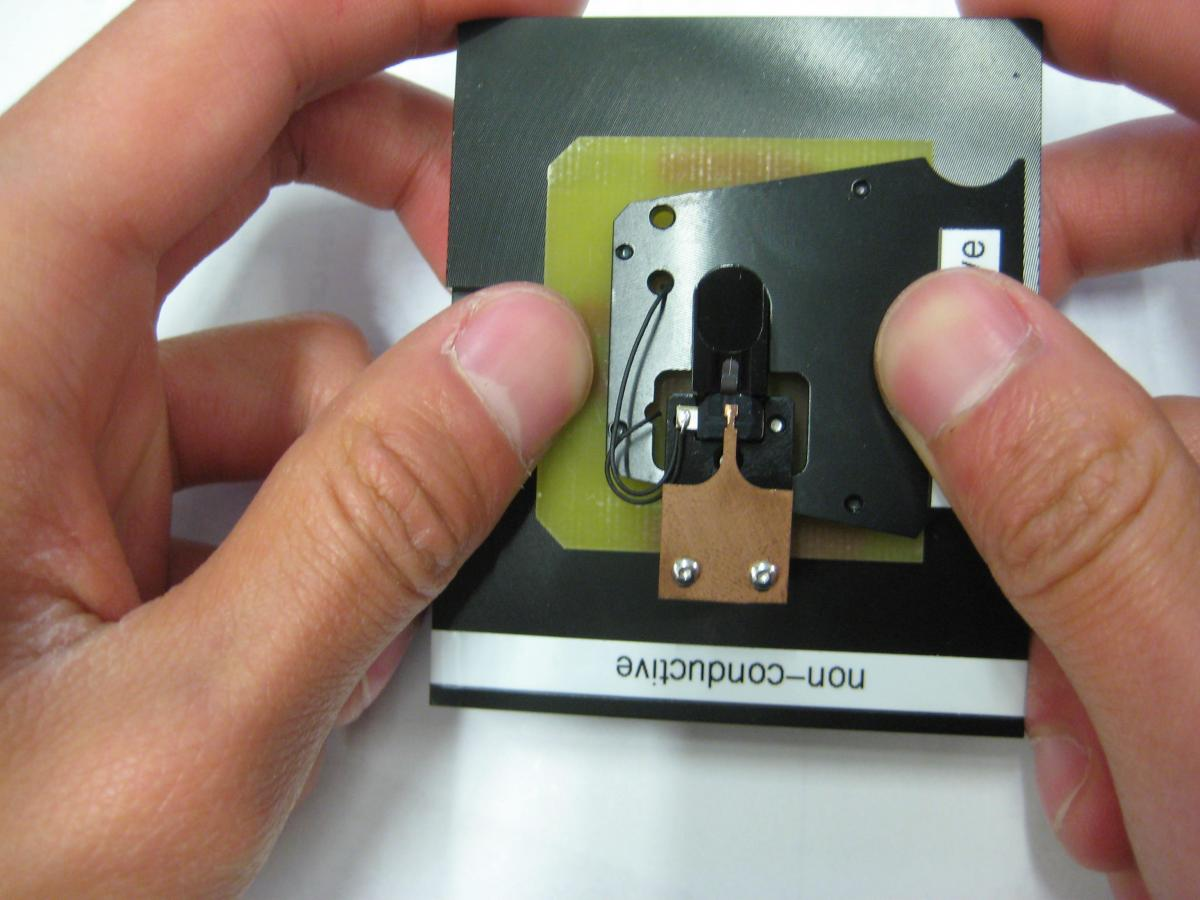
\includegraphics[width=0.5\linewidth]{images/22.JPG}}
        \caption{}
        \label{fig:22}
    \end{figure}
    
    \item  The probe should rest level in the back of the ``T'' track, and the front of the clip should be flush with the ``T crosshairs'' on the probe itself
    
    \begin{figure}[H]
    \begin{minipage}[t]{.5\linewidth}
        \centering
        \href{http://experimentationlab.berkeley.edu/sites/default/files/AFMImages/23.JPG}{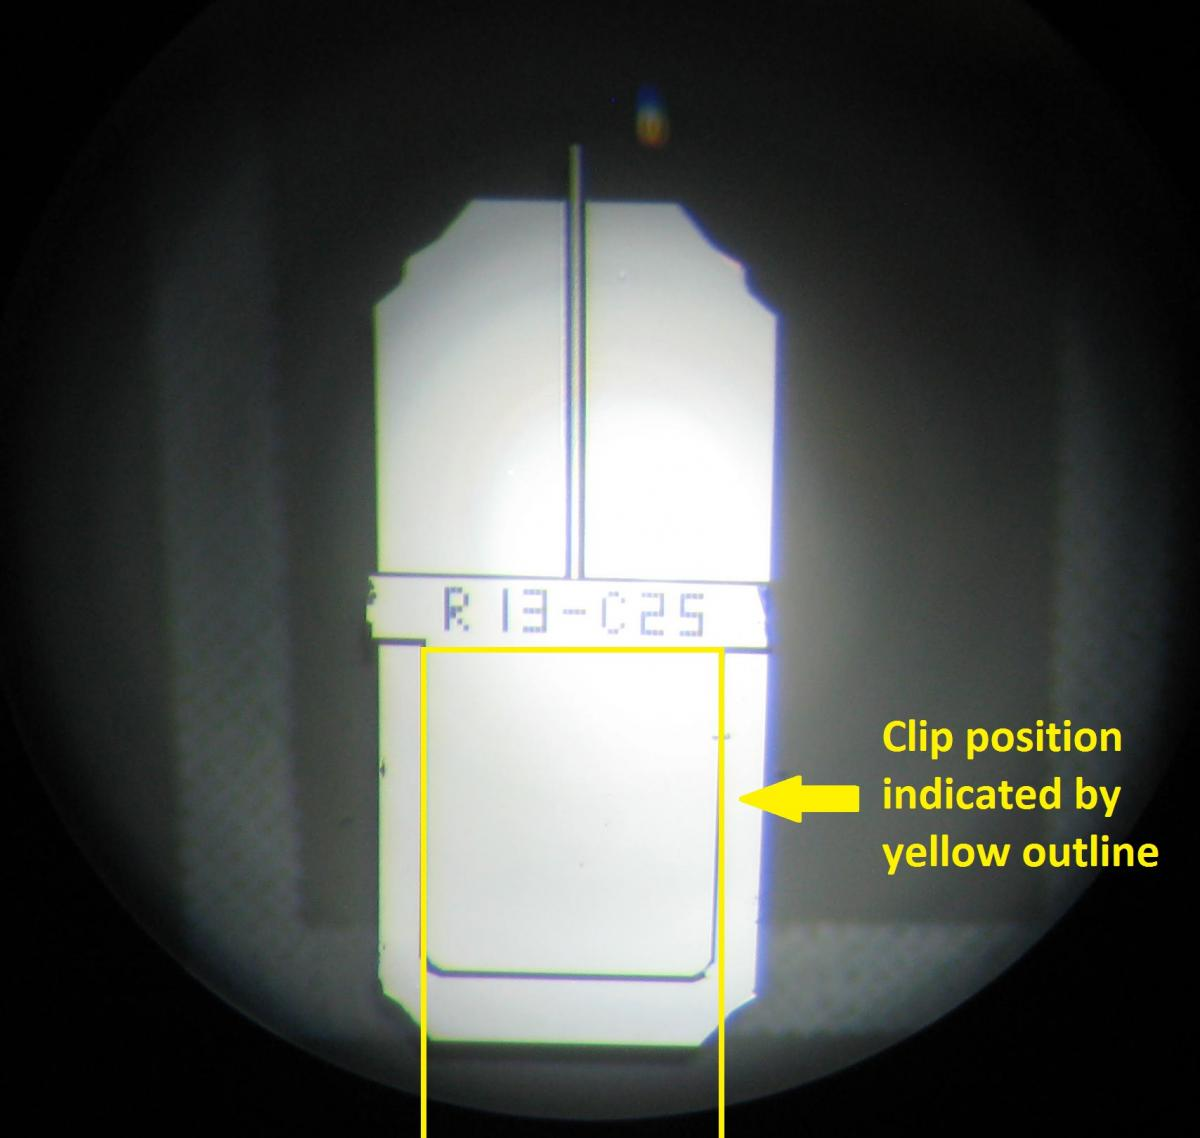
\includegraphics[width=0.8\linewidth,keepaspectratio]{images/23.JPG}}
        \caption{}
    \end{minipage}
    \begin{minipage}[t]{.5\linewidth}
        \centering
        \href{http://experimentationlab.berkeley.edu/sites/default/files/IMG_4053.JPG}{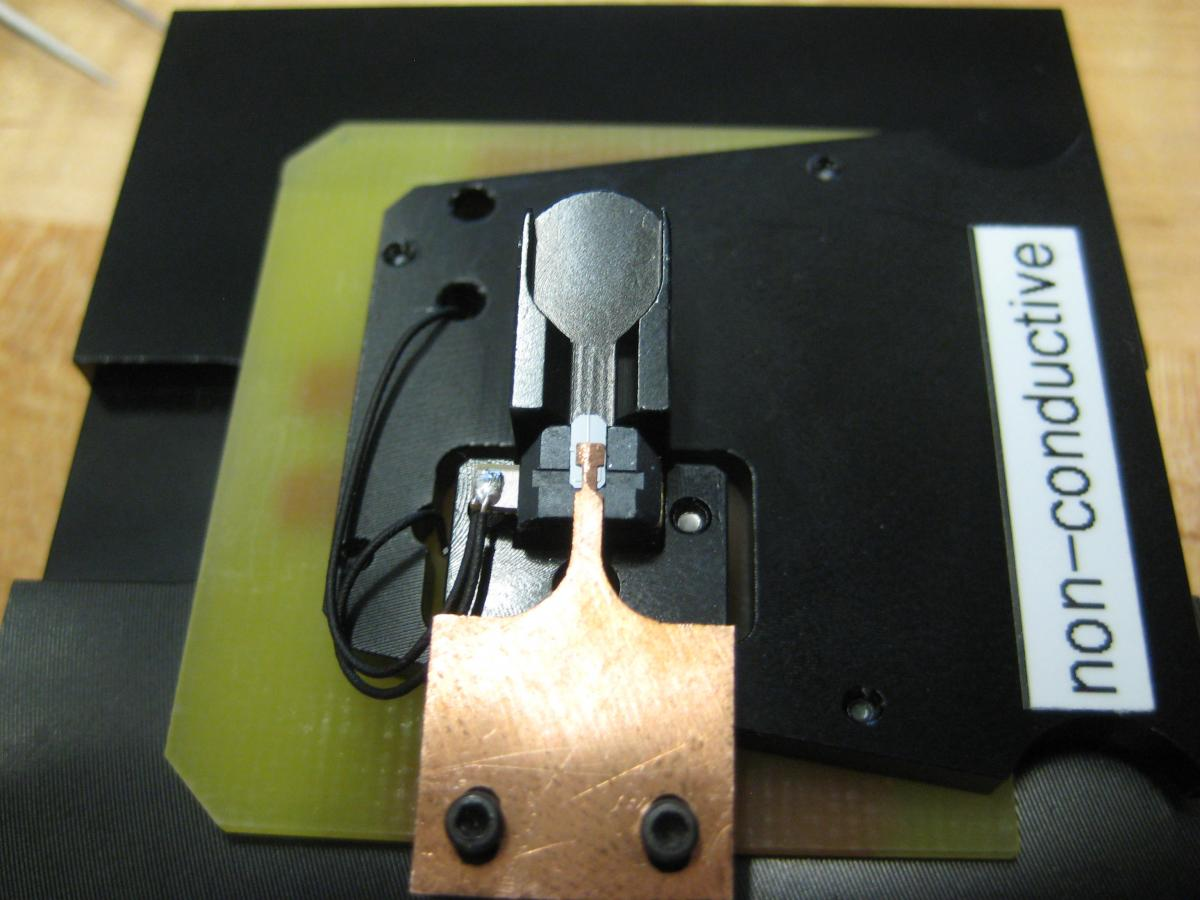
\includegraphics[width=0.8\linewidth,keepaspectratio]{images/IMG_4053.JPG}}
        \caption{}
    \end{minipage}
    \end{figure}
    
    \item  Release pressure of the probe holder on the exchange tool and \textbf{carefully} remove the probe holder from the exchange tool.
    
    \item \textbf{BEFORE} inserting the probe holder back into the AFM, \textbf{verify that there enough room for you to install the probe holder without hitting the sample holder (the metallic disk located on the stage)}.  Then Insert the probe holder with the new tip back into the TT-AFM with the \textbf{copper probe clip facing down}.
    
\end{enumerate}

\subsection{Changing Scanners}
\label{subsec:ChangingScanners}

If you want to change from the 15 Micron Scanner to the 50 Micron Scanner or vice versa, then follow these steps. Each scanner is appropriately labeled.

\begin{enumerate}
    \item First, raise the tip at least cm away from the scanner to give yourself lots of room to work with.

    \item Remove the probe holder, and carefully set it aside.

    \item Use the 3/16 Hex Wrench to loosen the 3 Hex Screws holding the scanner in place

    \begin{itemize}
        \item \textbf{DO NOT LOSE THESE SCREWS. KEEP THEM WITH THE SCANNER .}
    \end{itemize}

    \item CAREFULLY, unplug the ribbon cable from the back of the scanner

    \begin{itemize}
        \item Use caution when removing the cable \textbf{Grip the cable from the connector when removing to not damage the cable.}

    \end{itemize}

    \item Set this scanner aside.

    \item Take the desired scanner and first securely attach the ribbon cable in the rear.

    \item Align the scanner's hex screw holes with the base, and use the 3/16 hex wrench to tighten the hex screws.

    \begin{itemize}
        \item \textbf{IT DOES NOT NEED TO BE EXTREMELY TIGHT. JUST HAVE IT SECURE WITHOUT PUTTING STRESS ON THE SCREWS.}

    \end{itemize}

    \item Reinsert the probe holder into the TT-AFM.

\end{enumerate}

\section{Alignment}
\label{sec:Alignment}

\textbf{Centering Probe over Scanning Area/Sample Holder}

For this next section, refer to information in the top notch instructional video  \href{http://experimentationlab.berkeley.edu/sites/default/files/alignment\_final2.mp4}{\textbf{Alignment: Camera, Laser, and Detector}}.

Although there are written instructions below, your best bet is to watch the video above and follow along. Going slowly and surely through the alignment of the camera, laser and detector will \textbf{save you a lot of time} and \textbf{is essential} for getting good scans.

Before you load a sample, make sure the location of the tip is located in the center of the sample holder.  It is important to center the probe tip over the sample holder so that when the AFM takes a scan, vertical height will be recorded accurately.  If the probe tip is not centered, all 3D images produced from scans will be tilted.

The scanning area/sample holder is the silver disk located on the far right corner of the stage.  In the center of this disk is a screw.  You want to use the camera, and the x and y translators, to center the probe over the screw.  Follow the steps below to align the probe over the sample holder:

\begin{enumerate}
    \item Locate the probe on the Camera Viewer by adjusting the Camera Focus and Zoom.  The Focus knob on the AFM is labeled ``FOCUS'' and the Camera Zoom at the bottom of the black tube on the AFM is labeled ``Camera Zoom.''  Start by turning the Focus Knob all the way clockwise.  Then start turning the Focus Knob counterclockwise slowly until the probe comes into focus on the Camera Viewer (if you were to continue turning the Focus counterclockwise you would bring the probe's shadow on the sample into focus, which looks just like the probe but isn't because it's a shadow).  Then adjust the Zoom accordingly.

    \item Center the probe tip on the Camera Viewer.  Use the two Camera Adjustment Knobs labeled C1 and C2 to move where the camera is looking.
    
    \item We will use the Circle Tool on the Camera Editor to mark the position of the probe on the camera viewer. Click on the Circle Tool which looks like a circle with a red dot at it's center. Then move the mouse over the tip of the probe and click once.  Then move the mouse out to increase the size of your circle and then click again to set the circle.
    
    \item Turn the Focus knob counterclockwise to bring the camera focus down to the sample holder.  Keep adjusting the knob until the top of the screw on the sample holder comes into focus.
    \begin{itemize}
        \item When the screw is in focus, your Camera Viewer should look something like the image below:
        \begin{center}
            \href{http://experimentationlab.berkeley.edu/sites/default/files/AFMImages/sampleholder.PNG}{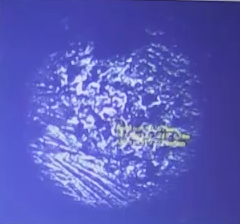
\includegraphics[width=0.5\linewidth]{images/sampleholder.PNG}}
        \end{center}
    \end{itemize}
    
    \item Use the X and Y micrometer knobs labeled S1 and S2 (which control the position of the Stage) to bring the yellow circle marker to the center of the screw.  Now you have centered the probe tip.
    
    \item Turn the Focus clockwise to bring the probe tip back into focus.  Note that the probe tip should still be located within the yellow circle.
    
    \item Click the left arrow on the camera editor (``Undo'') to remove the circle from the camera.
    
    \item Once you have centered the probe tip over the sample holder, try to avoid making further adjustments to the X and Y stage knobs S1 and S2 in order to keep the probe tip aligned.  This means that when you load the sample onto the sample holder, you want to load it in such a way that the scanning area of interest is located near the position of the tip, so you just have to move S1 and S2 a little bit.
\end{enumerate}

\subsection{Laser Align}
\label{subsec:LaserAlign}

After replacing a probe, you will have to realign the laser so that it properly reflects off of the cantilever.

\href{http://experimentationlab.berkeley.edu/sites/default/files/AFMImages/4.0\%20Laser\%20Align\%28V1.0\%29.wmv}{\textbf{This tutorial video}} quickly shows you how to align the laser using the laser adjustment knobs, in addition to our video  \href{http://experimentationlab.berkeley.edu/sites/default/files/alignment\_final2.mp4}{\textbf{Alignment: Camera, Laser, and Detector}}.  For additional detailed instructions, follow the steps below.

\begin{enumerate}
    \item Make sure you turned on the equipment and opened the appropriate programs. \hyperref[subsec:TurnOnInstrumentsAndOpenPrograms]{Directions are here.}

    \item Pull up the USB2.0 Camera Viewer. Make sure the \textbf{Preview} (Play button in upper left corner) is running (should be getting a live feed).

    \item Make sure the laser in the AFM is switched on in the AFM Workshop program, 2.0.3-15 Micron or AFM Workshop 2.4.15, in the \textbf{Pre Scan} tab in the \textbf{Laser Align} section.
    \begin{itemize}
        \item When you turn the laser on, you should see the laser reflecting off of the sample holder or probe holder in the AFM.

        \item DO NOT STARE DIRECTLY INTO THE LASER BEAM

        \item If you do not see the laser beam in the AFM, there might be something wrong with the laser and you should consult a GSI.
    \end{itemize}

    \item First, you need to locate the laser's position, relative to the probe.  On the optics tube of the AFM, zoom out the camera to 1.5x zoom.

    \item Turn the Focus knob until the probe and cantilever comes into focus.  Zoom out more if necessary.

    \item If you cannot see the laser beam on screen, spin the laser adjustment knob L1 \textbf{ }until the beam appears anywhere on the probe.  **\textbf{You should not need to turn the adjustment/micrometer knobs more than two revolutions either way.  }If you find yourself turning the knobs more than two revolutions, you should consult a GSI to help you find the laser beam on the camera viewer.
    \begin{itemize}
        \item The Adjustment Knob on top moves the laser in the X-Axis.
        \begin{itemize}
            \item Clockwise spin moves the beam in the -X-Axis direction (Left)

            \item Counterclockwise spin moves the beam in the +X-Axis direction (Right)
        \end{itemize}
    \end{itemize}

    \item Once the beam is somewhere on the probe, spin the laser adjustment knob L2 to bring the laser dot in line with the cantilever.  **\textbf{You should not need to turn the adjustment/micrometer knobs more than two revolutions either way.  }If you find yourself turning the knobs more than two revolutions, you should consult a GSI to help you find the laser beam on the camera viewer.

    \begin{itemize}
        \item The direction you spin the knob depends on where the beam first shows up.
        \begin{itemize}
            \item Clockwise spin moves the beam in the +Y-Axis direction (Up)

            \item Counterclockwise spin moves the bean in the -Y-Axis direction (Down)
        \end{itemize}
    \end{itemize}

    \item Once you have located the laser beam on the probe (looking at the Camera Viewer), you want to direct the laser beam along the length of the Cantilever.  Do this by slowly adjusting the L1 and L2 adjustment knobs.

    \item Zoom in the optics to $\sim$3.0x zoom.  Bring the probe into focus on the camera display again, using the Focus knob.

    \item Use both the L1 and L2 laser adjustment knobs to position the beam on the cantilever as shown in the photo below.
    \begin{itemize}
        \item \textbf{Make sure the beam is positioned before (to the right of) the triangle tip of the cantilever. } Imagine a crosshair at the triangle point of the cantilever--that is roughly where your tip is located.

        \item Center the beam, as best you can, between the top and bottom of the cantilever arm on the camera display.
        
        \begin{figure}[H]
        \centering
            \href{http://experimentationlab.berkeley.edu/sites/default/files/AFMImages/laser_align.png}{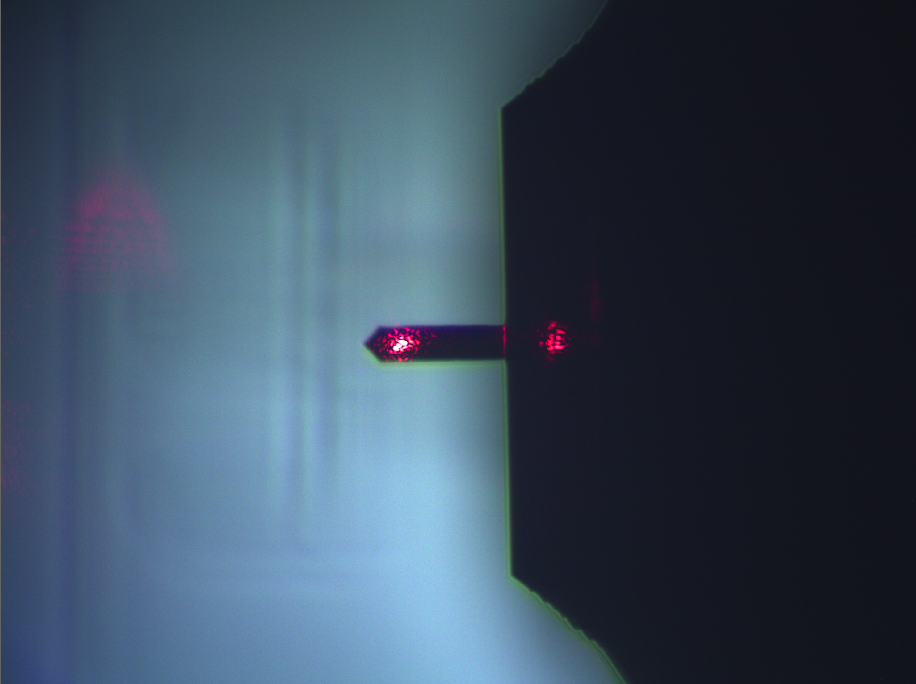
\includegraphics[width=0.5\linewidth]{images/laser_align.png}}
            \caption{Laser aligned on tip of cantilever}
            \label{LaserAlignment}
        \end{figure}
    \end{itemize}

\end{enumerate}

\subsection{Photodetector Alignment}
\label{subsec:PhotodetectorAlignment}

\href{http://experimentationlab.berkeley.edu/sites/default/files/AFMImages/5.0\%20\%20Phtodetector\%20Alignment\%28V1.0\%29.wmv}{\textbf{This video tutorial}} shows you how to align the laser using the photodetector adjustment knobs, in addition to our video  \href{http://experimentationlab.berkeley.edu/sites/default/files/alignment\_final2.mp4}{\textbf{Alignment: Camera, Laser, and Detector}}.

In the AFM program in the\textbf{ Laser Align} section of the \textbf{PreScan} Tab, the \textbf{Beam Position} tells you where the laser spot is hitting the photodetector. The Mean Adjustment is \textbf{D2}, this moves the beam horizontally on the Beam Position graph--moving the detector physically in or out.  We want D2 to move the red dot on the Beam Position to 0 horizontally.  This should be a one time adjustment.  If you have to change this that probably means that there is something wrong with the probe. \textbf{Top - Bottom should be around .3,} not 0.

\begin{center}
    \href{http://experimentationlab.berkeley.edu/sites/default/files/AFMImages/detectoralign.JPG}{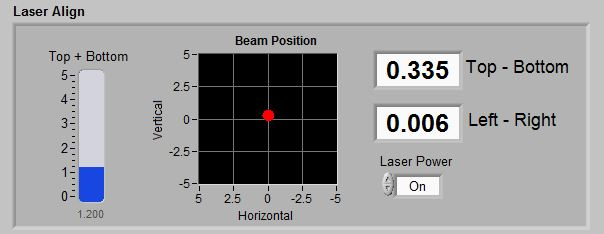
\includegraphics[width=0.65\linewidth]{images/detectoralign.JPG}}
\end{center}

\subsection{AFM Calibration (Complete on 1st Day)}

For your first scan, you will be taking a scan of the calibration slide so you can calibrate the AFM.

Cross reference the \href{http://experimentationlab.berkeley.edu/tt-afmuserguidev2.2}{\textbf{TT-AFM User Guide}}, Appendix C, pg.47 for additional directions on how to do a calibration

\textbf{Calibration Procedure:}

\begin{enumerate}
    \item Raise the tip a good distance (approx. 2 cm) above the sample holder by going to the \textbf{Manual Z Motor Control} of the \textbf{Pre Scan} Tab in the AFM program, raising the speed slider bar to a high value (above the halfway mark), and clicking and holding the \textbf{UP }button.  Refer to Figure~\ref{fig:PullOutYellowSlide}.  Then remove any sample (if applicable)

    \item Refer to the \hyperref[sec:Alignment]{Centering Probe over Scanning Area/Sample Holder} section above to make sure the Probe tip is centered over the screw located in the center of the sample holder.

    \item Verify that the the laser and detector are aligned by referring to the \hyperref[subsec:LaserAlign]{Laser Align} section and the \hyperref[subsec:PhotodetectorAlignment]{Photodetector Alignment} section located above.

    \item Insert Sample 7, labeled AppNano Silicon Step Height Reference, Part \# SHS-0.1-1

    \begin{itemize}
        \item Refer to \hyperref[subsec:HowToLoadASample]{How to Load a Sample Section} located below.

        \item Adjust the Camera Zoom to zoom out, so you can determine the orientation of the slide using the Camera Viewer.
    \end{itemize}

    \item Open the reference sample \href{http://experimentationlab.berkeley.edu/sites/default/files/AFMImages/Reference-\%20sample-SHS-01\_3\_datasheet.pdf}{\textbf{datasheet, here}}.

    \begin{itemize}
        \item Refer to the datasheet for the schematics of the reference sample, and the dimensions of its features.
    \end{itemize}

    \item \textbf{**This step is suggested but not necessary.**  }With the optics still zoomed out and the tip still raised high above the sample, CAREFULLY rotate the sample, WITHOUT accidentally touching the tip or the surface of the sample, so that it is oriented the same direction in your camera viewer as it is displayed in the datasheet schematic.  This makes identifying the features on the reference sample an easier task.

    \item Position a clean portion of the desired feature (refer below) on the reference sample under the tip of the cantilever.

    \begin{itemize}
        \item **Please refer to the \href{http://experimentationlab.berkeley.edu/sites/default/files/AFMImages/Reference-\%20sample-SHS-01\_3\_datasheet.pdf}{\textbf{datasheet}} to identify where each feature is located on the reference sample.**

        \begin{itemize}
            \item For the 15 Micron scanner, scan Feature A

            \item For the 50 Micron scanner, scan Feature B
        \end{itemize}

    \end{itemize}

    \item Verify that there is an approximate 2 cm separation from the sample and the probe holder, and then refer to the \textbf{} section located below to perform a Range Check. Then refer to the  section below to tune the Frequency and Phase.

    \item Refer to the  section located below to perform a Tip Approach.

    \item Click the \textbf{Topo Scan }tab, and perform a scan with the recommended Scan Setup settings as shown in Figure~\ref{fig:TopoScan}. (You may play around with these settings to see how the scan quality changes, or use your own preferred settings)

    \begin{itemize}
        \item Record the settings you used for your own reference

        \item Once this scan is completed, save your data to your preferred location

        \item Under Scan Setup, change the Rotation value from $0^\circ$to $90^\circ$ (IN THE SOFTWARE) and perform another scan.  Save your data to your preferred location

        \item Perform a Tip Retract by clicking the \textbf{UP} button in the \textbf{Tip Retract} Section to avoid \hyperref[subsec:BrokenTip]{damaging your probe}. \textbf{The scanning portion of the system calibration is now complete }
    \end{itemize}

\end{enumerate}

\textbf{Checkpoint. With the camera, show the staff the alignment of the laser on the cantilever, as well as the alignment of the sample stage. Show the staff the alignment of the detector as well. Show the staff your resonance data, as well as the peak you have chosen. Show the staff your image. Identify any debris or dirt.}

\textbf{Data analysis portion}

\begin{enumerate}
    \item Open the \hyperref[subsec:Gwyddion]{Gwyddion} data analysis/processing program.

    \item Perform steps 13-16 for both the $0^\circ$ and $90^\circ$ Z\_DRIVE scans. It is highly recommended to watch the \href{http://experimentationlab.berkeley.edu/sites/default/files/AFMImages/gwyddion1.mp4.mp4}{\textbf{gwyddion tutorial video}}.

    \item Level your data by fitting a plane through three points 
\includegraphics[height=2em]{images/44.png} and level rows using intersections with given lines 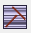
\includegraphics[height=2em]{images/46.png}

    \begin{itemize}
        \item Instructions and demonstrations on how to use these tools, and others, in Gwyddion are located below in \hyperref[sec:DataProcessingAndAnalysis]{Data Processing And Analysis} under Leveling
    \end{itemize}

    \item Using the Extract Profiles tool 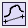
\includegraphics[height=2em]{images/profiles.png}, draw a profile across your neatest row (for $0^\circ$ scan) or column (for $90^\circ$ scan).

    \begin{itemize}
        \item Following the written instructions from \hyperref[sec:DataProcessingAndAnalysis]{Data Processing And Analysis}, or from the \href{http://experimentationlab.berkeley.edu/sites/default/files/AFMImages/gwyddion1.mp4.mp4}{\textbf{tutorial video}}, place a marker, from left to right, bisecting each feature at approximately the same point.  Record your length differences.

        \item According to the \href{http://experimentationlab.berkeley.edu/sites/default/files/AFMImages/Reference-\%20sample-SHS-01\_3\_datasheet.pdf}{\textbf{datasheet}},

        \begin{itemize}
            \item Feature A has a 3 micron pitch

            \item Feature B has a 10 micron pitch

            \item the reference slide as a whole has a height of 102.7nm
        \end{itemize}

    \end{itemize}

    \item Open the calibration program located in C:/AFM Experiment/AFM Calibration XYZ.html - Shortcut

    \begin{itemize}
        \item This will open an applet in Internet Explorer

        \item MAKE SURE you allow the applet to run in the Explorer (security popup at the bottom of the window)
    \end{itemize}

    \item Input your recorded length measurements for the X and Y Piezos as well as the actual values

    \item Using either your $0^\circ$or $90^\circ$ Z\_DRIVE scan profiles, place a marker at the top of the feature and another in the pit.  The height difference is shown under height in nanometers. Record and input your values into the calibration applet.

    \begin{itemize}
        \item do this for each different set of tops and pits until you have enough data to fill out the calibration applet.

        \item the Actual Z Piezo value is 102.7 (nanometers)
    \end{itemize}

    \item In the AFM scanning software, click the System tab.

    \item Under the calibration window, record the current calibration values

    \begin{itemize}
        \item refer and/or revert to these calibration values if your new calibration values are very off (they should be very, very close values to these)
    \end{itemize}

    \item Input the current system calibration values for XYZ into the Calibration Applet under the System Cal column.

    \item Click calculate, and \textbf{record your new XYZ calibration values}.

    \item ***\textbf{If clicking the Calculate button did not return New XYZ calibration values, MAKE SURE YOU HAVE ALL THESE VALUES ALREADY RECORDED.  Exit out of the Calibration applet and open it again, this time make sure you allow the applet to run when prompted by the web browser security pop up!***}

    \item Go back to the AFM scanning software and input the new calibration values into the System, Calibration window and click save.
\end{enumerate}

\textbf{Once you have performed a calibration you are ready to do the experiments.  After reading through the information and making sure you understand each procedure, jump ahead to the \hyperref[sec:Experiments]{Experiments} section.}

\subsection{How to Prepare a Sample}
\label{subsec:HowToPrepareASample}

**If the samples that you are going to use are already prepared (they most likely will be), you can \hyperref[subsec:TipApproach]{skip to the next step}.

\begin{enumerate}
    \item The small sample to be imaged must be less than 8mm thick, and must be able to fit on the adhesive tab on the sample disk (15mm diameter).

    \item The sample will be placed on the 15 mm metal disk

    \item It is very important for the sample to be kept as clean as possible so avoid touching it with your fingers.  When there is contamination of the sample, capillary forces pull the contamination up the probe, and pull the cantilever down.

    \item Use the provided double-sided adhesive tabs and tweezers.  Peel off one side of the adhesive protection backing and carefully attach it to the sample disk.  Next, peel off the other side, and use tweezers to place your small sample to be imaged firmly on the sticky tab.  Gently press the sample onto the sticky tab until secured.

    \begin{itemize}
        \item Make sure the area of interest is near the center of the disk

        \item Be sure that the sample is as flat as possible and that it does not protrude off the edge of the disk

        \item Alternatively, a small sample can also be glued to the sample disk using cyanoacrylate glue (superglue).
    \end{itemize}

\end{enumerate}

\subsection{How to Load a Sample}
\label{subsec:HowToLoadASample}

Watch \href{http://experimentationlab.berkeley.edu/sites/default/files/prescan\_final\_0.mp4}{\textbf{Pre-Scan: Tune Frequency, Tip Approach, and Scanning}}

\textbf{***BEFORE LOADING THE SAMPLE ONTO THE SAMPLE HOLDER, make sure that there is a large distance (at least 2 cms) between the probe and the sample holder.***}  You should turn the \textbf{Z Control} knob (located on top of the AFM near the camera tube) CLOCKWISE to raise the probe away from the sample holder.

\begin{itemize}
    \item Using the tweezers labeled ``Sample Use Only'', firmly grip the sample disk and place the prepared sample disk onto the sample holder then slide it into position.  Looking at the Camera Viewer, try to use the tweezers to move the area of the sample that you wish to scan as near as you can to the tip of the probe so you only need to make minor adjustments to the Stage's X and Y micrometers labeled S1 and S2.  Turning the S1 and S2 drastically in either direction will throw off the alignment preformed \hyperref[sec:Alignment]{here}.
    
    \item The metallic sample holder will magnetically attach to the stage, so be careful and aware when placing the disk on the stage, as to not damage anything.

    \item \href{http://experimentationlab.berkeley.edu/sites/default/files/AFMImages/3.0\%20Sample\%20Exchange\%28V1.0\%29.wmv}{\textbf{Basic Video Tutorial for step 5}}
\end{itemize}

\subsection{Setting up Pre-Scan Parameters for Vibrating Scan}
\label{subsec:SettingUpPreScanParametersForVibratingScan}

Watch \href{http://experimentationlab.berkeley.edu/sites/default/files/prescan\_final2.mp4}{\textbf{Pre-Scan: Tune Frequency, Tip Approach, and Scanning}}

\begin{enumerate}
    \item Make sure you are on the \textbf{Pre-Scan} tab in the program
    
    \item Set \textbf{Scan Mode} to \textbf{Vibrating} mode
    \begin{itemize}
        \item The \textbf{Tune Frequency} window becomes enabled
    \end{itemize}

    \item Focus the optics on the sample using the camera viewer.  You can adjust the magnification/zoom of the camera by turning the knob labeled\textbf{ ``Camera Zoom''} at the bottom of the large black tube positioned over the sample.  The focus of the camera is adjusted by the large black knob to the right of the black tube labeled ``\textbf{Focus''}.
    \begin{itemize}
        \item Clockwise rotation of the \textbf{Focus} knob raises up the camera's focus.
        \item Counter-clockwise rotation of the \textbf{Focus} knob lowers the camera's focus.
    \end{itemize}

    \begin{figure}[H]
        \centering
        \href{http://experimentationlab.berkeley.edu/sites/default/files/AFMImages/ZControl.jpg}{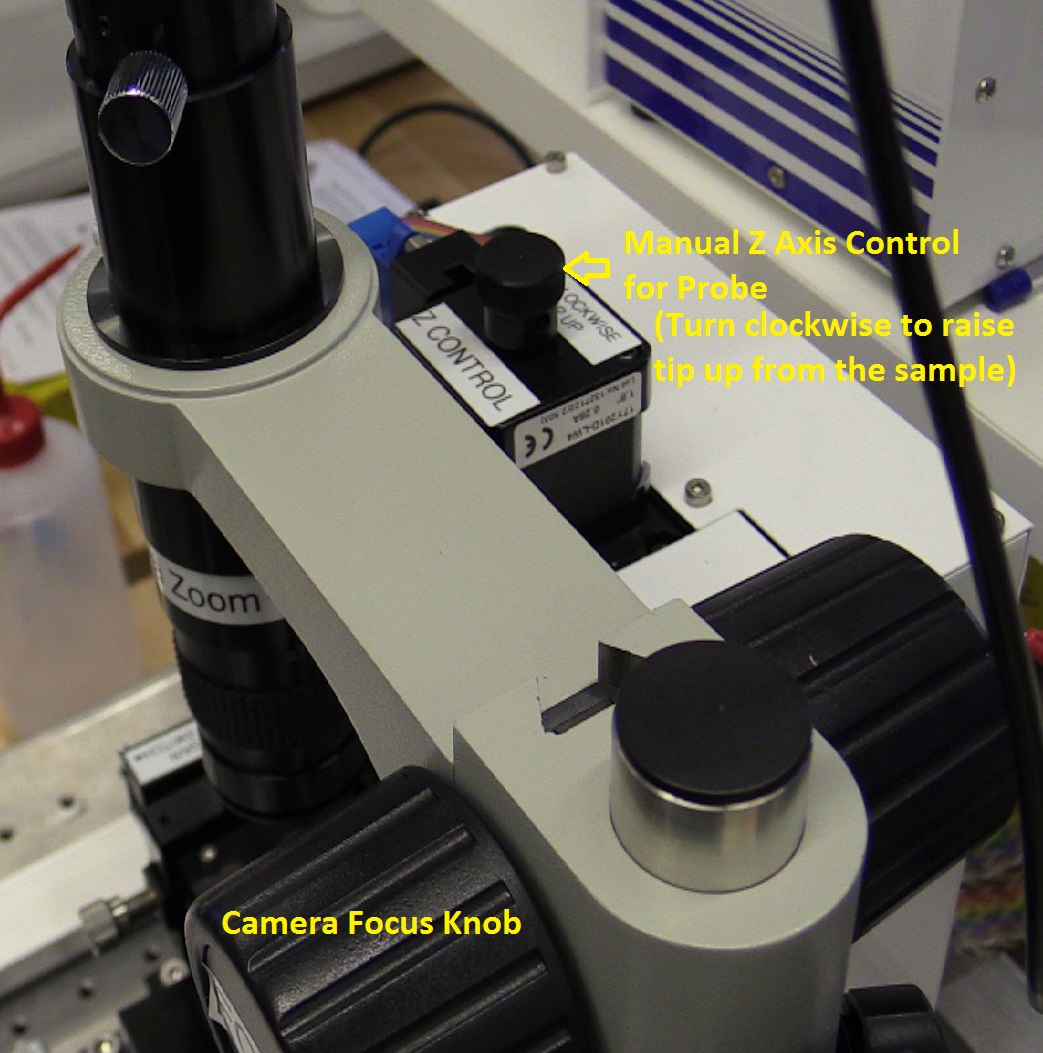
\includegraphics[width=0.5\linewidth]{images/ZControl.jpg}}
        \caption{AFM Knobs}
    \end{figure}
    
    \item\textbf{MAKE SURE THE TIP IS NOT TOO CLOSE TO THE SAMPLE} (if the sample is in focus with the camera, the tip should not be in focus--refer to Figure~\ref{fig:ProbeUnfocused} below). Make minimal adjustments to the X-Y micrometers labeled S1 and S2 to move the area of interest of the sample under the tip.
    
\end{enumerate}

\begin{figure}[H]
    \centering
    \href{http://experimentationlab.berkeley.edu/sites/default/files/AFMImages/26.png}{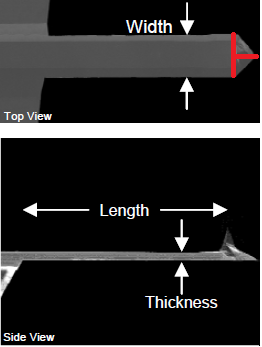
\includegraphics[width=0.5\linewidth]{images/26.png}}
    \caption{Top and side views of the cantilever}
\end{figure}

\begin{figure}[H]
    \centering
    \href{http://experimentationlab.berkeley.edu/sites/default/files/AFMImages/probe_unfocused1_0.png}{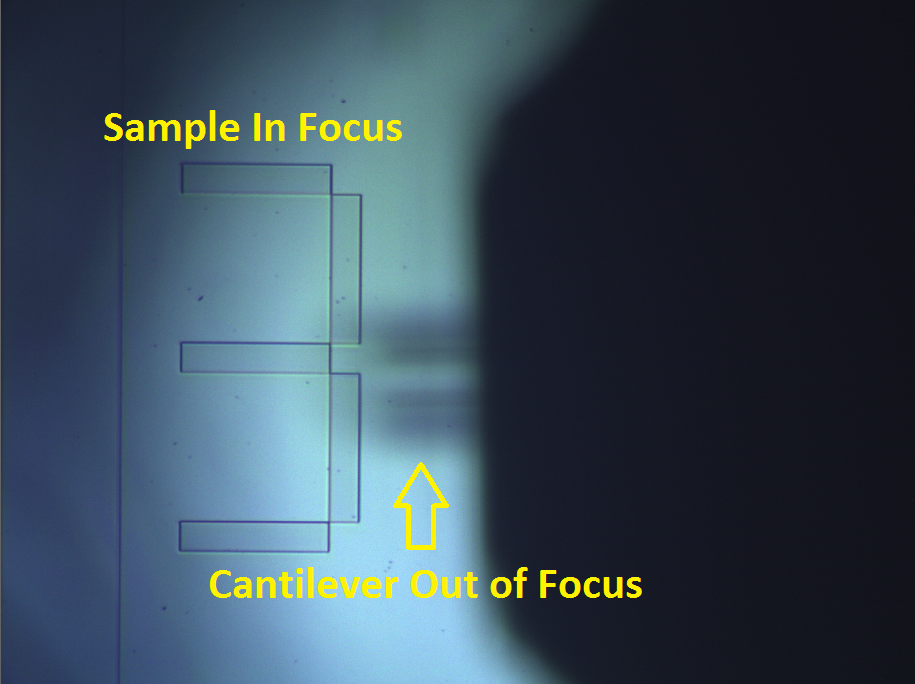
\includegraphics[width=0.5\linewidth]{images/probe_unfocused1_0.png}}
    \caption{The probe is not in focus while the sample is, meaning that there is a safe distance between the probe and the sample.  Adjust the focus of the camera so that your Camera Viewer resembles this figure.}
    \label{fig:ProbeUnfocused}
\end{figure}

\subsubsection{Range Check}
\label{subsubsec:RangeCheck}

(refer to \href{http://experimentationlab.berkeley.edu/sites/default/files/prescan\_final2.mp4}{\textbf{Pre-Scan: Tune Frequency, Tip Approach, and Scanning}})

Make sure the tip is NOT IN CONTACT with the sample (there should be about a 2 cm separation between the probe holder and the sample), then perform \textbf{Range Check} if indicator light is off
\begin{itemize}
    \item \textbf{Be sure that the tip is NOT IN CONTACT with the sample when running a range check because this will \hyperref[subsec:BrokenTip]{damage or destroy the tip}.}
    
    \item The sample moves as X and Y piezos initialize
    
    \item **During range check, the system ramps up the voltages to the x and y piezos, and captures the strain gauge output so that it can scan linearly. You have to do this, or you'll get bizarre scans and most likely \hyperref[subsec:BrokenTip]{break the tip}.
    
    \item **If you do not see the sample move in xy relative to the tip, there may be something wrong with the program.  Exit out of the program, power cycle the Ebox, then restart the program.
    
    \item The \textbf{Complete} light turns on when \textbf{Range Check} is finished
\end{itemize}

\subsubsection{Resonance Peak and Phase}

(refer to \href{http://experimentationlab.berkeley.edu/sites/default/files/prescan\_final2.mp4}{\textbf{Pre-Scan: Tune Frequency, Tip Approach, and Scanning}})

\begin{itemize}
    \item In the \textbf{Tune Frequency} window, under \textbf{Frequency Select} set Lower and Upper Frequencies to the Frequency range which is specified on the probe box. This will be the range the software sweeps over to find the probe's point of resonance.
    
    \item Each probe's specified frequency boundary should be located on the probe box
    
    \item Leave the \textbf{Selected }frequency anywhere in between this range
    
    \item Set the number of steps to be somewhere between 50-100
    
    \item Set the Demod Gain to 4dB
    
    \item Click the \textbf{Start} button to begin the frequency sweep
    \begin{itemize}
        \item\textbf{Resonance}
        \begin{itemize}
            \item On the upper oscilloscope (Amplitude v. Frequency), move green and red slider bars closer to the resonance peak
            
            \item This adjusts the sweep range
            
            \item Sweep the resonance peak again
            \begin{itemize}
                \item **Repeat steps 9 \& 10 as necessary until you achieve a resonance peak no greater than 2.5V**
                
                \item If the amplitude of the resonance peak exceeds 2.5V, adjust the driving amplitude of vibration by altering the \textbf{Amplitude} scroll bar.
            \end{itemize}
            
            \item Move the selected frequency (the blue slider on the oscilloscope) just to the left of the resonance peak (80\% up the left side of the resonance peak)
            
            \item Adjust \textbf{Amplitude (Vpp)} as needed to get a peak value between 1.00-2.00
            \begin{itemize}
                \item This fine tunes the position of the blue slider
                \item (sweep and adjust until the peak value is in the range)
            \end{itemize}

        \end{itemize}
        
        \begin{figure}[H]
            \centering
            \href{http://experimentationlab.berkeley.edu/sites/default/files/AFMImages/FreqPhase.JPG}{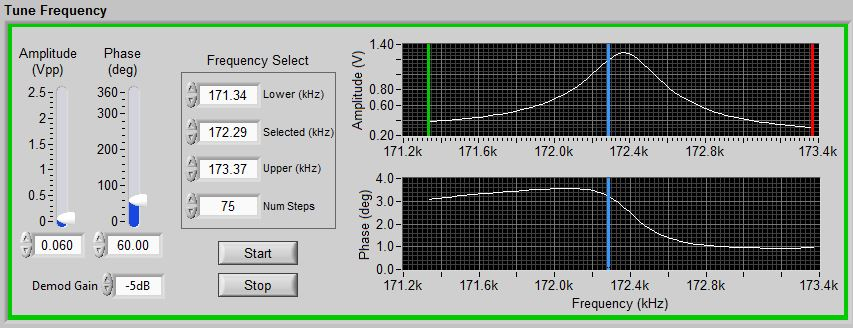
\includegraphics[width=0.8\linewidth]{images/FreqPhase.JPG}}
            \caption{Tune Frequency}
        \end{figure}
        
        \item\textbf{Phase}
        \begin{itemize}
            \item There should be an inflection point in the phase at the resonance peak.
            \item If this is not the case, to adjust the phase you will change the value in the Phase Slider bar labeled ``\textbf{Phase (deg)}'' in the \textbf{Tune Frequency }section of the \textbf{Pre Scan} tab. Try changing the value to 0, 90, or 180, and each time perform a sweep by clicking on the \textbf{Start} button and see if the point of inflection lines up with the resonance peak.  If the inflection point is close to lining up, try adjusting the ``\textbf{Phase (deg)}'' minutely either way (try 10 degrees) to get it to match up.  To make the sweep go faster you can decrease the \textbf{Num Steps.}
            \item Aligning the point of inflection of the Phase with the resonance peak is critical if you will be measuring/displaying \textbf{Z Phase }during a scan in the \textbf{Topo }\textbf{Scan }tab.
        \end{itemize}
        
    \end{itemize}

\end{itemize}

\textbf{Checkpoint: Call a GSI over and show them the settings you have selected here prior to performing a tip approach.}

\subsection{Tip Approach for Vibrating Mode}
\label{subsec:TipApproach}

(first manual, then automated) (refer to the video \href{http://experimentationlab.berkeley.edu/sites/default/files/prescan\_final2.mp4}{\textbf{Pre-Scan: Tune Frequency, Tip Approach, and Scanning}})

**NOTE: For non-vibrating mode, make sure you have ``N\emph{on-Vibrating''} selected under \emph{Scan Mode} in the Pre Scan Tab.  The rest of the tip approach process is the exact same as Vibrating Mode, except that you will not need to do a \emph{Tune Frequency} because the probe will not be vibrating in this mode.

**NOTE: Depending on the sample's reflectiveness, it may be more or less difficult to gauge the focus of the probe tip, and therefore the probe's distance from the sample. Keep this in mind and proceed with caution as you perform a tip approach.**

\begin{enumerate}
    \item Bring the probe closer to the surface, \emph{BUT DO NOT MAKE CONTACT WITH THE SAMPLE!} Use the \textbf{Down} button in the \textbf{Manual Z Motor Control} section of the \textbf{Prescan} tab to lower the tip to the sample until the tip is just slightly out of focus (the sample should be in focus with the camera).
    \begin{itemize}
        \item \textbf{Make sure to not crash the tip into the sample when manually lowering the tip before the Automated Tip Approach. This can \hyperref[subsec:BrokenTip]{damage and/or destroy the tip}.}
        \begin{itemize}
            \item \textbf{**if the laser spot in the detector becomes un-centered, with the laser red spot significantly up above the center, you have crashed your tip into the sample.}
        \end{itemize}
    \end{itemize}
    
    \item You can visually check the distance or use advanced methods
    Advanced method mentioned in the \href{http://experimentationlab.berkeley.edu/tt-afmuserguidev2.2}{\textbf{TT-AFM user guide,}} pg.25 section 4.5-4.5.1
    
    \item Speed of motor is adjustable with the slider bar
    \begin{itemize}
        \item **It is advised that the slider bar be set all the way to the left at the slowest setting.  The indicator will read zero, but the motor will still move (should be able to hear the motors activate).
    \end{itemize}
    
    \item\textbf{Be conscious to not crash the tip into the sample using manual motor controls. This will \hyperref[subsec:BrokenTip]{damage or destroy the tip}.}
    
    \item **If you feel comfortable with the instrument, having the tip closer to the sample before the automated tip approach will mean a shorter waiting time**
    
    \begin{figure}[H]
        \centering
        \href{http://experimentationlab.berkeley.edu/sites/default/files/AFMImages/probe_unfocused2_0.png}{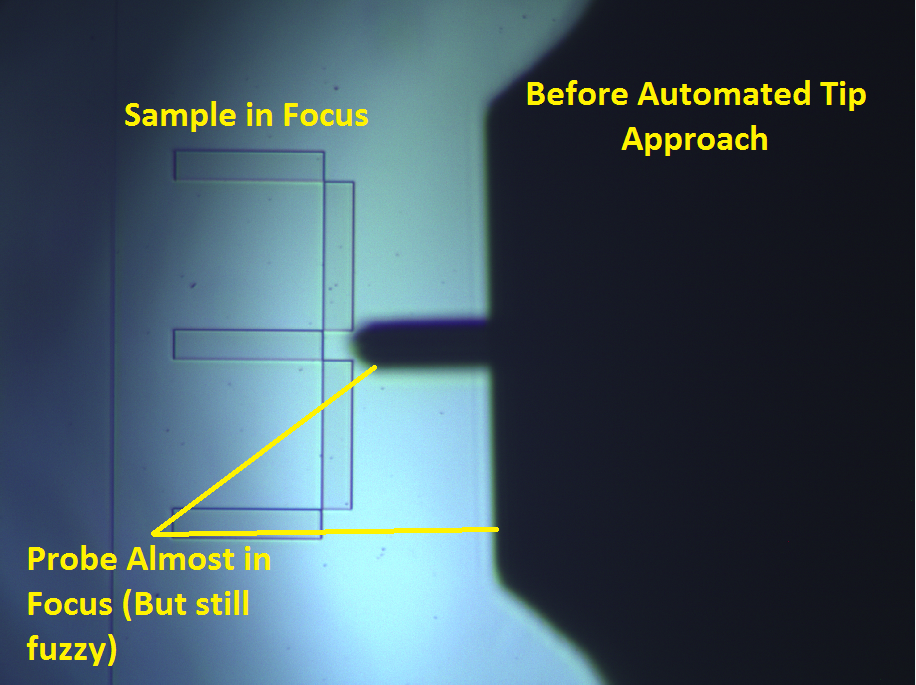
\includegraphics[width=0.5\linewidth]{images/probe_unfocused2_0.png}}
        \caption{}
    \end{figure}
    
    \item Ensure the that resonance frequency of the probe has already been selected. \textbf{Ensure the that the laser is on.} You may now initiate the automated tip approach
    
    \item Press the \textbf{Start} button in the \textbf{Automated Tip Approach }section to begin
    
    \item Tip approach can be observed in the \textbf{Z Drive} indicator. You will notice the yellow indicator alternates between top and bottom as the tip approach commences.
    
    \item The feedback indicator light will turn on when tip approach is complete
    
    \item If the feedback indicator light is flickering on and off, go to the \textbf{System }Tab, in the \textbf{Other Controls} section find the \textbf{Feedback Limit }value.  Increase this value by .01 and then check if the feedback indicator is still flickering.  If it is still flickering, repeat this step until it is the in feedback loop is consistently illuminated.
    
    \item Tip approach takes a few minutes from a tip to sample height of $\sim$1mm.  Completion time will depend on how close the tip is to the sample before tip approach.
    
    \item\textbf{STOP!} After the automated tip approach has finished and the in feedback light is illuminated:
    \begin{itemize}
        \item To ensure that the tip is actually engaged with the sample, and is not in ``false feedback'' (where the system thinks it is engaged, but in reality it is not) locate the \textbf{Setpoint (mV) }value in the \textbf{Automated Tip Approach} section. Lower this value by increments of 10 and observe the yellow bar. You should not lower the setpoint more than 30 (lowering it by 10 three times). If the tip is engaged with the sample, the yellow bar will not move in position. If it begins to slowly drift noticeably upward, then unfortunately, the system is in false feedback. If you find the system is in false feedback, you must use the manual z motor control to move the tip up until it goes out of feedback and then re-do the tip approach. Before reinitiating tip approach, the yellow bar should be near 10 V in the Z Drive indicator, and the in feedback light should be off. After these criteria are met, click up on the manual z motor control 3 more times, \textbf{go to the system tab of the Software and lower ``extend factor'' in ``Tip Approach Parameters'' by .05,} then reinitiate a new automated tip approach. If you find that the tip is indeed engaged with the sample, you will now have one of three tasks, outlined below:
        \begin{enumerate}
            \item The yellow bar in the Z Drive indicator is centered at zero. If this is the case you are ready to begin your scan in the topo scan tab.
            
            \item The yellow bar in the Z Drive indicator is above zero. If this is the case, go to the \textbf{Topo Scan }Tab and in the \textbf{Z Feedback }section change the \textbf{Integral }value from 1000 to 100 (\emph{you will change this value back to 1000 for your scan}).  Then go back to the \textbf{Pre Scan }Tab and by the \textbf{Automated Tip Approach }section click on the \textbf{Re-Center} button.  If the \textbf{Re-Center }function times out, you can try clicking on \textbf{Re-Center }again to see if it works.  If the \textbf{Re-Center }function does not bring the yellow \textbf{Z Drive }indicator to 0 (the center of its range), you will want to go to the \textbf{Manual Z Motor Control }section and click on the \textbf{UP }button a few times until the probe tip is $\sim$1 mm away from the sample.  Then reinitiate the the \textbf{Automated Tip Approach} and start over. This can be a pain, but it is essential to have the Z Drive indicator centered and the tip engaged with the sample.
            
            \item The yellow bar in the Z Drive indicator is below zero. If this is the case, use the manual z motor control section to move the yellow bar up in the Z Drive indicator. You want the in feedback light off and the yellow bar near 10 V. Click up on the manual z motor control three more times. Reinitiate tip approach.
        \end{enumerate}
    \end{itemize}
    
\end{enumerate}

\begin{figure}[H]
    \centering
    \href{http://experimentationlab.berkeley.edu/sites/default/files/AFMImages/bothfocused.jpg}{\includegraphics[width=0.5\linewidth]{images/bothfocused.jpg}}
    \caption{}
\end{figure}

\textbf{***ACLA PROBES ARE DESIGNED FOR NON-CONTACT, TAPPING MODE, INTERMITTENT CONTACT, AND/OR CLOSE CONTACT APPLICATIONS***}

\subsection{Topography Scanning}

\begin{enumerate}
    \item Make sure you are in vibrating mode, and did a vibrating mode tip approach. \hyperref[subsec:SettingUpPreScanParametersForVibratingScan]{Click here for directions}.
    
    \item Click the \textbf{Topo Scan} tab
    
    \item Set parameters and settings to match those in the screenshot below
    \begin{itemize}
        \item \textbf{**NOTE only pay attention to the values in the text boxes. Ignore the tip retract and Z Drive position indicators in Figure~\ref{fig:TopoScan} below for this step**}
    \end{itemize}
    
    \begin{figure}[H]
        \centering
        \href{http://experimentationlab.berkeley.edu/sites/default/files/AFMImages/toposcansetup.jpg}{\includegraphics[width=0.7\linewidth]{images/toposcansetup.jpg}}
        \caption{}
        \label{fig:TopoScan}
    \end{figure}
    
    \item Begin a scan by clicking the \textbf{Start} button in the \textbf{Scan} window
    \begin{itemize}
        \item The probe will move into position and the scan will begin
        
        \item Captured data is displayed in the graphs above
        
        \item Progress of the scan is displayed in the counter next to \textbf{Scan Lines} in the \textbf{Scan Setup} window
    \end{itemize}
    
    \item The scanned image will be displayed as a \textbf{mirrored image}, reflecting over the y-axis, relative to the actual orientation and position of the sample.
    
    \item When scan is complete, change the file name and save path as desired
    
    \item\textbf{**TO SAFELY DISENGAGE THE TIP, CLICK THE UP BUTTON IN THE TIP RETRACT SECTION**}
    \begin{itemize}
        \item When the tip retract completes, the green indicator light will turn on
    \end{itemize}
    
    \item If you want to scan a different area on the sample or remove the sample, go to the \textbf{Pre Scan }tab and click on the \textbf{UP }button in the \textbf{Manual Z Motor Control }Section to raise the tip a safe distance from the sample.  There should be >1 cm separation between the sample and the probe, to not \hyperref[subsec:BrokenTip]{damage the tip}.
\end{enumerate}

Scanning times for 15 Micron scanner:

\begin{table}[H]
    \centering
    \begin{tabular}{l|l|l}
        Scan Lines & Scan Frequency & Scan Time \\\hline
        128 Lines  & 1 Hz           & 2 minutes \\\hline
        128 Lines  & 0.5 Hz         & 4 minutes \\\hline
        256 Lines  & 1 Hz           & 4 minutes \\\hline
        256 Liens  & 0.5 Hz         & 8 minutes \\\hline
        512 Lines  & 1 Hz           & 8 minutes \\\hline
        512 Lines  & 0.5 Hz         & 16 minutes
    \end{tabular}
    \caption{}
\end{table}

\section{Data Processing and Analysis}
\label{sec:DataProcessingAndAnalysis}

AFM images are a 3D array of numbers which represent the surface of the sample.  There are 3 types of functions for this data:
\begin{enumerate}
    \item Display: Changes how the numbers are viewed
    
    \item Process: Changes the numbers in the array
    
    \item Analysis: Extracts numbers from the data array
\end{enumerate}


Use the program \textbf{Gwyddion} to view, process, and analyze your data:
\begin{figure}[H]
    \centering
    \href{http://experimentationlab.berkeley.edu/sites/default/files/AFMImages/39.png}{\includegraphics[width=0.3\linewidth]{images/39.png}}
    \caption{Gwyddion program measurement icons}
    \label{fig:GwyddionProgram}
\end{figure}

Watch the \href{http://experimentationlab.berkeley.edu/sites/default/files/AFMImages/gwyddion1.mp4.mp4}{\textbf{Video tutorial for Gwiddion here}}

\subsection{Gwyddion (Data Processing/Analysis)}
\label{subsec:Gwyddion}

\textbf{NOTE: If you wish to do some of your post processing at home, or on your own/another computer, you may COPY (do NOT manipulate the folder) the Gwyddion program folder (about 60Mb) from the AFM computer onto your USB drive.  The folder is located in C:/AFM Experiment, named Gwyddion.  The .exe required to run the program is located in the folder as Gwyddion/bin/gwyddion.exe}

\textbf{Note to Don: The original Gwyddion folder is buried deeper in this computer, in case the one located above is accidently corrupted.}

\begin{itemize}
    \item Open the Gwyddion.exe program located in the AFM Experiment folder on the C drive.
    
    \item Open the data files you previously saved (file extension .wsf) in Gwyddion by clicking file$\rightarrow$open$\rightarrow$wherever you saved the file
    \begin{itemize}
        \item Select the left image (Z\_DRIVE)
    \end{itemize}
    
    \item\textbf{NOTE: Save processed data files as native Gwyddion files.}
    \begin{figure}[H]
        \centering
        \href{http://experimentationlab.berkeley.edu/sites/default/files/AFMImages/40.png}{\includegraphics[width=0.5\linewidth]{images/40.png}}
        \caption{Sample imported AFM scan in Gwyddion}
    \end{figure}
    
    \item Click the \includegraphics[height=2em]{images/41.png} button under the \textbf{View} drop down menu to view your data in 3D.
    \begin{itemize}
        \item You can manipulate the view of your data using these buttons and clicking and dragging the image around in the window.
        
        \item Right click on the image to pick a fun color setting, to make things more fun.
        
        \begin{figure}[H]
            \centering
            \href{http://experimentationlab.berkeley.edu/sites/default/files/AFMImages/42.png}{\includegraphics{images/42.png}}
            \caption{Click the floppy disk to save your 3D image}
        \end{figure}
    \end{itemize}
    
    \item You will use the 3D image of your data as a reference as you process your data to accurately represent your sample.
    
    \item **Be able to identify what features on the image are actually part of your sample's surface and which are artifacts or contaminants.**
    \begin{figure}[H]
        \centering
        \href{http://experimentationlab.berkeley.edu/sites/default/files/AFMImages/43.png}{\includegraphics[width=0.5\linewidth]{images/43.png}}
        \caption{}
    \end{figure}
    
    \item\textbf{Leveling:} When you look at the 3D projection of your image, you will notice that your sample is tilted. If you know your sample is FLAT (or parts of it are flat), you can use the tools in the \textbf{tools} dropdown to fix the tilt, else go to step 4.
    \begin{itemize}
        \item \includegraphics[height=2em]{images/44.png} Level data by fitting a plane through three points
        \begin{itemize}
            \item Click three different points on your sample's image which you know to be FLAT (e.g. the substrate). Click \textbf{apply} to process the data.
            
            \item Beware of artifacts and debris being scanned with your image.  Do not place your markers on them, or try to avoid them because they will distort your data.
            
            \item **notice the change on your 3D image**
            
            \item Check the \textbf{Set plane to zero} checkbox when leveling out the substrate.
            
            \item You can level other known flat surfaces by clearing out the three points with the \textbf{Clear} button, then selecting three new points and applying again.
            \begin{itemize}
                \item Clicking \textbf{Clear} will not undo, your previous levels. (Crtl+Z to undo)
                
                \item Other known flat surfaces include the surfaces of 2D materials (e.g. graphene as pictured below)
                \begin{figure}[H]
                    \centering
                    \href{http://experimentationlab.berkeley.edu/sites/default/files/AFMImages/45.png}{\includegraphics[width=0.5\linewidth]{images/45.png}}
                    \caption{}
                \end{figure}
            \end{itemize}
            
        \end{itemize}
        
        \item \includegraphics[height=2em]{images/46.png} Level rows using intersections with given lines
        \begin{itemize}
            \item Draw lines through scan lines that you know are level.
            \begin{itemize}
                \item Draw lines from top to bottom, covering the length vertically
                
                \item The lines do not need to be continuous, but need to cover the whole length vertically
            \end{itemize}
            
            \item Be careful to not draw the lines through artifacts or dust/debris on your image. This will lead to incorrect data processing.
            \begin{figure}[H]
                \centering
                \href{http://experimentationlab.berkeley.edu/sites/default/files/AFMImages/47.png}{\includegraphics[width=0.5\linewidth]{images/47.png}}
                \caption{}
            \end{figure}
            
        \end{itemize}
        
        \item Surface Subtract?
        
    \end{itemize}
    
    \item Under the \textbf{Data Process} drop-down, there are various controls used to auto-process your image. Level the image and correct for unwanted lines and scars using the following buttons.
    \begin{itemize}
        \item \includegraphics[height=2em]{images/48.png}
    
        \item The order in which they are clicked \emph{does} matter
        
        \item Trial and error until you achieve a desirable image
        \begin{itemize}
            \item Ctrl+Z to undo an image process
        \end{itemize}
        
    \end{itemize}
    
    \item **You can change the color scheme of your images by right-clicking the color scale bar on your Z\_DRIVE image and directly on your 3D image.  This may be easier to work with because it makes features easier to identify.
    
    \item Measure the profile of your scan by using the \textbf{Extract Profile} tool \includegraphics[height=2em]{images/profiles.png} in the \textbf{Tools} dropdown menu.
    \begin{itemize}
        \item Draw your profile along your area of interest.  The profile will be plotted in a graph x (length) vs y (height) along this line. Click \textbf{Apply} and a new window should pop up.
    \end{itemize}
    
    \begin{figure}[H]
        \centering
        \href{http://experimentationlab.berkeley.edu/sites/default/files/AFMImages/49.png}{\includegraphics[width=0.5\linewidth]{images/49.png}}
        \caption{}
    \end{figure}
    
    \item In the new window, click the \textbf{Measure distances in graph} button \includegraphics[height=2em]{images/50.png} and use your cursor to place markers by clicking on the points of interest on the graph of the profile.
    
    \begin{figure}[H]
        \centering
        \href{http://experimentationlab.berkeley.edu/sites/default/files/AFMImages/51.png}{\includegraphics[width=0.5\linewidth]{images/51.png}}
        \caption{}
    \end{figure}
    
    \begin{itemize}
        \item The extracted values are
        \begin{itemize}
            \item the intersection coordinates of each marker with the profile
            \item the distance (length) between the two markers
            \item the height difference between the two markers
        \end{itemize}
    \end{itemize}
    
    The mentioned methods in this lab write-up are just the main tools you can use to process and analyze the data.  You are not limited to just these tools, there are other tools in the gwyddion software that you can explore if you have the time.
\end{itemize}

\subsection{Image Merging}
\label{subsec:ImageMerging}

Given the limited scan size of a scanner, you can use software to combine multiple scans of a sample to one data file to measure, edit, etc.  Image merging relies heavily on software, so having scans that are very easy to stitch together is pretty rare because the user cannot manually adjust how the images are stitched together.  Height data tends gets skewed during image merging because the software will force different scans to fit together, which may be slightly different from one another.  This is just another tool that you may try to analyze your data.
\begin{enumerate}
    \item First, complete all of your scans using the AFM.  Make sure that all of your scans overlap, so that the software is able to identify and stitch together your scans based on identifiable features.
    
    \item Open all of the Z\_DRIVE scans that are to be merged together in Gwyddion (File $\rightarrow$ Open) in the same order that they were scanned to reduce confusion later on.
    \begin{itemize}
        \item It may be helpful to click and drag the scan windows and place them in the order that you will stitch them together to grasp mentally.
    \end{itemize}
    
    \item Make sure that your scans are processed in Gwyddion (level to plane, line leveling, fix to zero) before continuing
    
    \item Once all of the scans are open, select the first scan by clicking on it, we will begin here.
    
    \item In Gwyddion Figure~\ref{fig:GwyddionProgram}, under File, Edit, click \textbf{Data Process} $\rightarrow$ \textbf{Multidata }$\rightarrow$ \textbf{Merge}.
    
    \item A pop up will open:
    \begin{itemize}
        \item click the \textbf{Merge with:} drop-down menu and select the next adjacent Z\_DRIVE scan.
        \item click the \textbf{Put second operand:} drop-down menu and select the position that the next scan will be, relative the the first scan.
        \item set \textbf{Align second operand:} to \textbf{Correlation}, and set \textbf{Boundary treatment:} to \textbf{Smooth}
    \end{itemize}
    
    \item Click \textbf{OK}, and a Gwyddion will merge your scans and display a new scan.
    
    \item Select the new merged data image and repeat steps 5-8 until you have merged all of your original scans.
    
    \item Using the Crop tool \includegraphics[height=2em]{images/33.png}, crop the final scan so that the black spaces generated from the merging are removed.
    
    \item The data can now be manipulated and measured just like another scan.
    
    \item\textbf{NOTE: It is very likely that your merged scan is imperfect.  Beware of these descrepencies as you analyze your data to make sure that your measurements make sense, and are not just blind measurements that include artifacts from the merge.}
\end{enumerate}

\section{Experiments}
\label{sec:Experiments}

For any of these experiments, you may use the overhead microscope to get an overview of the samples. It is recommended to do this for experiments that require scanning over a particular area on the sample.

\emph{\textbf{In this lab you will perform FOUR of the following experiments in addition to measuring Boltzmann's Constant which is REQUIRED (5 experiments total).}}

\begin{enumerate}

\item \hyperref[subsec:NoiseFloor]{Noise Floor Experiment}

\item \hyperref[subsec:CD/DVD]{CD/DVD Experiment}

\item \hyperref[subsec:CarbonCrystal]{Carbon Crystalline Structure Experiment}

\item \hyperref[subsec:Microcircuit]{MicroCircuit Experiment}

\item \hyperref[subsec:GlueStick]{Glue Stick Polymer Experiment}

\item \hyperref[subsec:ForceDistance]{Force-Distance Experiment}

\item \hyperref[subsec:Boltzmann]{Spring Constant of the Cantilever and Measuring Boltzmann's Constant}

\end{enumerate}

\textbf{Checkpoints: Choose 2 of the experiments other than the Boltzmann's Constant experiment and explain to a GSI what you did and describe some of your results. These are two separate checkpoints, one for each experiment.}

\subsection{Noise Floor Experiment}
\label{subsec:NoiseFloor}

This short experiment is designed to show you how your physical behavior and environmental variables will affect the outcome of your measurements.

\textbf{Use Sample 8, Blank Silicon Wafer, for this experiment.}

Use either scanners, or both if you have time. \hyperref[subsec:ChangingScanners]{(How to change a scanner)}

Use a Z HV Gain value of 5 for this experiment.

\begin{enumerate}
    \item Take a \hyperref[subsec:MeasureNoiseFloor]{noise floor measurement} in a very quiet environment (closed box, no talking, no touching the table, no leg shaking, etc.) and record your noise floor.

    \item Take another noise floor measurement in a noisier environment (box open, talking to your partner, typing/writing on the table, etc.) and record your noise floor.

    \item Which has the larger noise floor? Why? (lower is better)

    \item FFT analysis of your noise floor:

    \begin{enumerate}
        \item Locate the .wsf data files of both your noise floor scans.

        \item Complete steps 3-6 for both of your scans

        \item Open Microsoft Excel, then click and drag your .wsf data file into Excel workspace.  The parameters of your scan and a matrix of the data points should appear.

        \item Highlight a \textbf{Row} of data and copy it.  You should use one of the rows in the middle of your dataset, and not ones near the top or bottom.  This is the data for a single scan line

        \item Perform a Fast Fourier Transform (FFT) to this line of data in the way of your choosing (Excel, Matlab, Python, by hand, etc.)
        \begin{itemize}
            \item You may wish to do steps 4-5 for multiple rows of data from a single scan, for this will confirm that the general trend of the FFT is similar
    
            \item If you do not know how to do this, you may refer to this \href{http://experimentationlab.berkeley.edu/sites/default/files/AFMImages/afm\_freq.m}{\textbf{sample Matlab script}}.
        \end{itemize}

        \item Plot your results, and save your plot to include in your lab write-up
    \end{enumerate}

    \item Now that you see the most common frequencies of noise, what can you extrapolate about different the sources of noise affecting this experiment?

    \item Can you identify and explain the different measures that the lab has taken to reduce the noise for the AFM experiment? (Examine the experiment table.)

    \item What are other ways and precautions that you can take to lower the noise floor when scanning your sample with AFM?

\end{enumerate}

\subsection{CD/DVD Experiment}
\label{subsec:CD/DVD}

\textbf{Use Samples 1, and 2 (CD With Data and DVD Sample respectively) for this experiment}

\textbf{INSERT PDF education sample kit page 6, 7}

\textbf{Use the 15 Micron Scanner} \hyperref[subsec:ChangingScanners]{(How to change a scanner)}

\begin{enumerate}
    \item Begin with a few sources - explain how a CD works and what we are expecting to see. The following are external links and are not exhaustive on this topic. (Destructive/Constructive interference)

    \begin{enumerate}

        \item \href{http://experimentationlab.berkeley.edu/sites/default/files/How\%20Information\%20is\%20Stored\%20on\%20a\%20CD.mp4}{\textbf{How Information is Stored on a CD}}

        \item \href{http://experimentationlab.berkeley.edu/sites/default/files/Bits_and_CDs.pdf}{\textbf{Bits and CDs}}

        \item \href{http://experimentationlab.berkeley.edu/sites/default/files/How_do_Rewriteable_CDs_work.pdf}{\textbf{How do rewriteable CDs work?}}

    \end{enumerate}

    \item \emph{Before you scan, explain and include in your write-up: How is information is stored on a CD? What wavelength of light is used? Why? How is it different for a DVD? Explain constructive and destructive interference as well as a brief explanation of EMF. Using your knowledge, find an expected value for pit depth of the CD/DVD. You will compare this number with your measurement during the lab. }

    \item ``Each pit is approximately 125 nm deep by 600 nm wide, and varies from 850 nm to 3.5 $\mu$m in length.The distance between the tracks, the pitch, is 1.6 µm.''

    \item A 780 nm laser is used to scan CDs

    \item Scan the CD with Data sample. Save data/image

    \item Scan the DVD Sample with the same scan size.  Save data/image

    \item Correct raw scan data in gwyddion

    \item Describe the features on the CD and DVD scans, what are they? Use your data, include in your write up an image and label different features

    \item Verify the depth of the pits for constructive/destructive interference. How do the measured depths of the pits compare to your expectation from step 2?  Explain any similarities or differences you find.  (refer to \href{http://experimentationlab.berkeley.edu/sites/default/files/How_do_Rewriteable_CDs_work.pdf}{\textbf{source 3}})

    \begin{itemize}
        \item ​​\textbf{NOTE: The CD sample was mounted on upside down, so the pits will appear as bumps instead.  The dimensions are unaffected.  The DVD sample still appears as pits.}

    \end{itemize}

    \item Verify the width between tracks. How does your measured value compare with the expected width?

    \item Measure lengths of different features and explain why they vary in length and what they mean (refer to sources).  How is the data actually stored in a disk?

\end{enumerate}

\subsection{Carbon Crystalline Structure Experiment}
\label{subsec:CarbonCrystal}

\textbf{Use samples 5, 6, 14 (Graphene, HOPG, Graphite) for this experiment}

\textbf{INSERT PDF education sample kit page 3-5}

\textbf{Use the 15 Micron Scanner} \hyperref[subsec:ChangingScanners]{(How to change a scanner)}

\begin{enumerate}
    \item Take scans of each of the three samples and save your data along with images of each (Z\_DRIVE).

    \begin{itemize}
        \item Sample 5 (graphene) has small graphene flakes (greenish color) on top of of a Silicon wafer substrate (purplish color). \textbf{Be sure to scan a flake of graphene and NOT the silicon wafer}.

        \item Be sure you know which data belongs with which sample.  \textbf{The data file cannot be opened if renamed improperly. Have some method of keeping track of your data.}
    \end{itemize}

    \item Measure the surface roughness of each sample in \hyperref[subsec:Gwyddion]{Gwyddion}, using the Statistical Quantities tool \includegraphics[height=2em]{images/36.png}
    \begin{enumerate}
        \item Open your Z\_DRIVE image in gwyddion.

        \item Click the Statistical Quantities tool

        \item Highlight the area of interest you wish to take a surface roughness measurement of on your Z\_DRIVE scan.
        \begin{itemize}
            \item A marquee should box this area
        \end{itemize}

        \item Record the Ra (Sa) value. This is your surface roughness
    \end{enumerate}

    \item The Ra value is given by the equation $R_a=\frac{1}{n} \sum\limits_{i=1}^{n} |y_i|$ where $n$ is the total number of pixels in the area for calculation, and $y$ is the Z axis height of each of the points in the image.

    \item These are all composed of the same element, carbon, so why do they display such different surface characteristics? What can you say about the ordering of the atoms for each of these three samples?

    \item Do your observations same make sense when you compare them to the actual crystalline structure for each of these samples? (look for images of crystalline structure on the internet)

    \item Give an example of why someone would want to use AFM to examine surface roughness in real life.

\end{enumerate}

\subsection{MicroCircuit Experiment}
\label{subsec:Microcircuit}

\textbf{Use sample 4, Microcircuit Siddiqi Lab, for this experiment}

\begin{enumerate}
    \item View the MicroCircuit under the optical microscope to understand the circuit's structure. Cross-reference this with the schematics on \href{http://experimentationlab.berkeley.edu/sites/default/files/AFMImages/CSQ\_Resonators\_1July2011\%20.pdf}{\textbf{data sheet}}.

    \item In the Systems tab of the scanning software, change the Z HV Gain to a value of at least 10.  This is because the vertical features on this sample are relatively large and we want the AFM to be able to compensate for these large changes at a reasonable pace without returning inaccurate data.

    \item Take multiple scans (minimum of 4, but more scans can be \textbf{stitched} together easier and more accurately), spanning across a trace (insert photo) of the circuit.  Make sure your scans overlap, this is crucial for merging your data.

    \begin{itemize}
        \item \textbf{CAUTION: Remember to perform a tip retract before moving the sample with the micrometers to avoid breaking a tip. Multiple tip retracts may be necessary to clear the tip from the features on the sample.}

        \item Remember the scale at which you are scanning at. A seemingly small adjustment with the micrometers will result in a large shift in your scan image. Moving the sample too far in one turn can result in you losing your scan position.  This will most likely mean that you must re-scan across the entire trace again.

    \end{itemize}

    \item Because the 15 micron scanner cannot span across these the traces, you must correct each scan and \hyperref[subsec:ImageMerging]{merge} them together in \hyperref[subsec:Gwyddion]{Gwyddion}.

    \item Measure the merged and corrected data's features using tools in Gwyddion

    \begin{itemize}
        \item \textbf{NOTE: The merging feature in Gwyddion is an imperfect tool.  Sometimes scans will merge seamlessly. Other times they will not merge properly at all. You must have a general idea of what the features of your scan should look like to determine if your merged data is usable or not.}
        \begin{itemize}
            \item \textbf{When taking measurements of the merged scan, you must take these flaws into consideration.  Use your knowledge of geometry to extrapolate the actual dimensions of your scans.}
        \end{itemize}

    \end{itemize}

    \item Do these dimensions that you measured of your scan match up with the dimensions given in the \href{http://experimentationlab.berkeley.edu/sites/default/files/AFMImages/CSQ\_Resonators\_1July2011\%20.pdf}{\textbf{data sheet}}?

    \item What is the height of the features on this microcircuit?  This value is not given in the data sheet.

    \item What does the feature that you scanned do? (look at sheet)

    \item Print out the schematic of the microcircuit from the data sheet and identify the area that you scanned by boxing it.

    \item Although the geometric coupling structure is identical for all the multiplexed resonators, Qc varies with fo, resulting in a range of coupling values.

\end{enumerate}

\subsection{Glue Stick Polymer Experiment}
\label{subsec:GlueStick}

You should read up on the physics behind a phase measurement in AFM in the \href{http://experimentationlab.berkeley.edu/sites/default/files/AFMImages/Lecture\_10\_AFM.pdf}{\textbf{Lecture 10 PDF}}, pg.40-45

\textbf{INSERT PDF education sample kit page 12-14}

\textbf{Use Sample 12, Hot Glue, for this experiment.}

\textbf{Use the 50 Micron Scanner} \hyperref[subsec:ChangingScanners]{(How to change a scanner)}

\begin{enumerate}
    \item Under Scan Setup, set your Scan Size to $\leq$ 15 $\mu$m

    \item Scan the sample, with the left image set to Z\_DRIVE and the right image set to Z\_PHASE.

    \begin{itemize}
        \item If you wish to examine larger images of your scans in the scanning software, click the \textbf{``S''} button on the right side of each image, above the amplitude scale, to enlarge your images.  (click it again to close it)

        \item You may overlay your images by switching the\textbf{ ``OFF''} button to \textbf{``ON''} under the Display window in the Topo Scan tab.  Adjust the transparency percentage to your own preference.  Overlaying the images will not affect your raw data.

        \item Save your data. (This only saves each of your scans independently, and \emph{not} the overlaid image).
    \end{itemize}

    \item Examine your Z\_PHASE data; differences in phase correlate to the hardness/softness of different regions in your scan.

    \begin{enumerate}
        \item Cross examine your Z\_PHASE data with your Z\_DRIVE and/or overlaid scan.  Does an increase in phase correlate to a relatively harder or softer material? Explain why.

        \item How many different polymers can do you think you can identify in your scan, based on the different phases?
    \end{enumerate}

\end{enumerate}

\subsection{Force-Distance Experiment}
\label{subsec:ForceDistance}

\textbf{Use the 50 Micron Scanner} \hyperref[subsec:ChangingScanners]{(How to change a scanner)}

Force/Distance curves are created by measuring the deflection of the cantilever as the sample is moved towards and then away form the probe at the end of the cantilever.  The shape of a F/D curve depends primarily on the cantilever stiffness and the thickness of a surface contamination layer.

**see animation \href{http://experimentationlab.berkeley.edu/sites/default/files/AFMImages/Force-distance\_curves\_en\_video.mp4}{\textbf{Force Distance Curve 01}} (this link brings you to a new page, open link in new tab)

Here is another animation showing a \href{http://experimentationlab.berkeley.edu/sites/default/files/AFMImages/6.1\%20Tip\%20Sample.flv\_converted.mp4}{\textbf{Force Distance Curve 02}}.


\textbf{Atomic Interaction (Forces):}

    \begin{itemize}
        \item Repulsion – A very strong repulsive force is present between the tip and sample atoms when the tip-sample distances are very small (level of only a few angstroms).  This is due to exchange interactions caused by overlapping electron orbitals on the atomic scale.

        \begin{itemize}
            \item The tip and sample are considered to be in \textbf{Contact} when repulsive forces are predominant.

        \end{itemize}

        \item Attraction (Van der Waals) – An attractive interaction is created between atoms when the instantaneous polarization of an atom induces the polarization in other nearby atoms. (polarization interaction).

        \item Friction – The cantilever on the probe will bend laterally due to frictional forces between the tip and the sample surfaces (Lateral Force Microscope LFM).

        \item Adhesion – Adhesion can be defined as ``the free energy change to separate unit areas of two media from contact to infinity in vacuum or in a third medium.''

        \begin{itemize}
            \item The pull-off force is considered as the adhesion force, ranging from a few nanonewtons to tens of nanonewtons.

            \item Adhesion is the cause of meniscus forces, where the tip wants to snap-in to place due to relative humidity, which creates a thin layer of water on the sample's surface
        \end{itemize}

        \item Electrostatic – Caused by both the localized charges and the polarization of the substrate due to the potential difference between the tip and the sample.

        \begin{itemize}
            \item Used to study electrostatic properties of samples such as microelectronic structures, charges on insulator surfaces, or ferroelectric domains.
        \end{itemize}

        \item Magnetic – Caused by magnetic dipoles both on the tip and the sample. This interaction is used for Magnetic Force Microscopy to study magnetic domains on the sample surface.

    \end{itemize}

More info in\textbf{ }\href{http://experimentationlab.berkeley.edu/sites/default/files/AFMImages/Lecture\_10\_AFM.pdf}{\textbf{Lecture 10}} pg.17-21

\textbf{Procedure for taking a Force Distance Curve:}

\begin{enumerate}
    \item If you haven't already, perform a \textbf{Tip Retract}. The Probe must not be in contact with the sample.

    \item Use the 50 micron scanner, and AFM Workshop 2.4.15.exe

    \item Under the \textbf{System} tab, change the Z HV Gain to 5.  This value is suggested for this sample, but you may explore other ones if time permits.

    \item Under the \textbf{Pre-Scan} tab, switch the \textbf{Scan Mode} to \textbf{Non-Vibrating}

    \item \textbf{Because you changed the Z HV Gain, do a range check}

    \item Perform a \hyperref[subsec:TipApproach]{non-vibrating tip approach}.
    \begin{itemize}
        \item Make sure that the AFM is \textbf{In Feedback} and that the \textbf{Z Drive} is centered.
    \end{itemize}

    \item Click on the \textbf{Force-Distance} tab.
    \begin{itemize}
        \item These are the settings by default.
        \begin{center}
            \href{http://experimentationlab.berkeley.edu/sites/default/files/FD.png}{\includegraphics[width=0.9\linewidth]{images/FD.png}}
        \end{center}
    \end{itemize}
    
    \item Make sure you are in Feedback Mode under the Force-Distance tab
    
    \item Initiate the Force/Distance measurement by clicking the \textbf{Start} button
    \begin{itemize}
        \item When the measurement is finished, the status bar on top will read ``Complete'' and it will automatically stop
        
        \item You will be prompted to save your data, which will save as a .csv file that can be opened with either Excel or Text Editor.
    \end{itemize}
    
    \item Take multiple scans so you can have an average for your data.

\end{enumerate}

\subsubsection{Procedure for Force Distance Experiment}

\textbf{Use sample 8, Blank Silicon Wafer}

\begin{enumerate}
    \item **Make sure you are in non-vibrating mode, and you do a \hyperref[subsec:TipApproach]{non-vibrating tip approach} in the Pre Scan before you begin your Force-Distance measurement.**

    \item perform a force distance measurement on the blank silicon wafer sample.

    \begin{itemize}
        \item Save your force-distance data when prompted

        \item right click to save an image of your data as well (but it can be later reproduced from your saved data in Excel, MatLab, Python, etc.)

    \end{itemize}

    \item Why is your x-axis (vertical movement) not starting from zero?  At which point does the probe come in contact with the sample surface?

    \item Does your sample have contamination? How can you tell from your measurement?

    \item Plot the points from the data file, using the program of your choosing (Excel, Matlab, Python, etc.) and fit a curve to the sloped part of your data.

    \item What is the voltage/expansion relation of the z-piezo?

    \item Find the total adhesion force between the sample and the probe tip, due to surface contamination.

\end{enumerate}

\subsection{Spring Constant of the Cantilever and Measuring Boltzmann's Constant}
\label{subsec:Boltzmann}

THIS IS A REQUIRED EXPERIMENT

The manufacturer, AppNano, provides a range of resonant frequencies and spring constants for their probes. These are listed on the box that contains the probes. Modeling the cantilever as a simple harmonic oscillator gives a relation between spring constant k and resonant frequency, $\omega_r$ (what is it?). Using the endpoints of the range of frequencies and the range of spring constants gives you two points along this curve. Using the point (0,0) will give you a third point. Interpolating these three points with a Lagrange polynomial (use Wolfram alpha) yields the exact relation predicted by the model. The AFM software allows for a good measurement of $\omega_r$. Plugging this into your polynomial will give you the spring constant k.

\textbf{Measuring Boltzmann's Constant:}

The cantilever is very sensitive to forces. Since we are operating it in ambient conditions, the cantilever is constantly bombarded by air molecules. Thermal fluctuations cause random cantilever deflections. Measuring these deflections will allow us to calculate Boltzmann's constant.

The equipartition theorem relates the temperature of a system to the energy stored in its various degrees of freedom. In the case of the cantilever, we can model it as a one-d harmonic oscillator bobbing up and down. In this case, there is one degree of freedom (no translational motion, no twisting, etc.). The energy in the one degree of freedom is that of a spring with spring constant $k$: $PE = \frac{1}{2} k z^2$ Therefore, we know that the average potential energy is related to the temperature by $PE = \frac{1}{2} k \langle z^{2} \rangle = \frac{1}{2} k_b T$, where $k$ is the spring constant of the cantilever and $k_b$ is Boltzmann's constant. You just measured $k$. For $T$, check the thermometer next to the EBOX. This leaves you to measure $\langle z^2 \rangle$.

In order to measure $\langle z^2 \rangle$, we will use the 15 $\mu$m scanner. Set the scan rate to .1Hz. Scan in non-vibrating mode for around 10 lines. Save the data.

Open the data up in Gwyddion. Extract an image profile with the ``Extract Profiles'' tool under the tools section. Make sure that the line you draw to extract a profile is level (as you draw the line for the profile, make sure that y1 and y2 in the profiles window are the same). Click apply. A new window will pop up with your profile.  By right clicking the image in the new window, ``level'' the data. Then right click again and click on Export Text. Hit OK and save the file with a .txt extension. Make sure that the file directory is in \textbackslash AFM Experiment\textbackslash 2.0.3 - 15 Micron AFM Workshop\textbackslash Test Data

We will use MATLAB to calculate the mean square deflection.

Open up MATLAB. Navigate to the directory in which you saved the file. That will allow access to your data as well as some scripts. Now, call the function ``mean\_sq'' on your text file, surrounded in single quotes.

Example: My data is in the text file mydata.txt. I type in mean\_sq(`mydata.txt').Voila.

You can check out the power density spectrum by calling the function bolt on your text file (again, in single quotes).

Use the value returned by mean\_sq to calculate Boltzmann's constant.

\textbf{Checkpoint: Show a GSI the procedure you used to determine the spring constant, and explain how you'll use these values to measure Boltzmann's Constant.}

\section{Data Analysis}

Compare the different spring constant values found in this lab, along with the the manufacture specs, and explain your results.  Given what you have learned about AFM in this experiment, you should be able to explain what is going on.

Take into consideration the limitations of the instrumentation as well as what the equations mean. Discuss how this AFM takes measurements, and what its limitations are. (Hint: investigate noise floor. take more noise floors if necessary)

It is good to think about how the software makes calculations to better explain the values used, rather than just taking numbers that you know know what they mean.

\subsection{Imaging Artifacts}

Include some examples of  artifacts and debris present in your scans and explain how they affected your measurements.  What caused these errors to occur, and how does it affect your data?

Refer to \href{http://experimentationlab.berkeley.edu/sites/default/files/AFMImages/Lecture\_10\_AFM.pdf}{\textbf{Lecture 10}}  pg.46-49

\href{http://experimentationlab.berkeley.edu/sites/default/files/AFMImages/AFM\_image\_artefacts.pdf}{\textbf{AFM image artifacts}} (images and captions do a good job of explaining it)

\subsection{Measure Noise Floor}
\label{subsec:MeasureNoiseFloor}

The noise floor measurement will let you know the limit at which your scans will be able to distinguish actual features from inherent noise of the AFM (electric or mechanical).  Ideally, this should be below 1 nm.

\begin{enumerate}
    \item In this next section you will make changes to your scan parameters in the Topo Scan tab.  To not lose any of your scan settings, record your current values for Scan Size, Scan Rate, Scan Lines, and X, Y Center.  You will use these values later if you decide to take another scan.

    \item Make sure the tip is a sizeable distance from the surface of the sample.  Initiate the \textbf{Tip Retract }function if necessary, or use the manual Z motor control.

    \item Click the \textbf{Systems} tab. \textbf{(DO NOT CHANGE THESE SETTINGS AFTER YOU HAVE INITIATED A TIP APPROACH.  YOU MUST PERFORM A TIP RETRACT BEFORE CHANGING THESE VALUES BACK OR YOU WILL \hyperref[subsec:BrokenTip]{BREAK A TIP})}
    \begin{itemize}
        \item Under \textbf{XY Parameters}, change the value of the \textbf{XY HV Gain} to 0

        \item Under \textbf{Z Parameters}, change the value of the \emph{\textbf{Z HV Gain}} to 7
    \end{itemize}

    \item Click the \textbf{Topo Scan} tab.  Set scan parameters to:
    \begin{itemize}
        \item Scan Size = 0.5 microns

        \item Scan Rate = 1 Hz

        \item Scan Lines = 512

        \item X, Y Center = (2, 2) for 50 micron scanner, or (0.5, 0.5) for 15 micron scanner

        \item Left, Right Image = Z-Drive, Z-Error
    \end{itemize}

    \item If not already in focus, using the Manual Z motor Control in the Pre-Scan tab, move the probe toward the sample until the probe begins to come into focus.

    \item Complete an \textbf{Vibrating mode} Automated \hyperref[subsec:TipApproach]{Tip Approach}.

    \item Begin a scan.  It is not necessary to complete the whole scan.
    \begin{itemize}
        \item 50 scan lines is plenty.
    \end{itemize}

    \item To analyze the noise floor measurement, open the Z-Drive scan in Gwyddion.
    \begin{itemize}
        \item \hyperref[sec:DataProcessingAndAnalysis]{See next section} (Data Processing and Analysis) about accessing Gwyddion.
    \end{itemize}

    \item Crop the data if necessary. \includegraphics[height=2em]{images/33.png}

    \item Level the image by pressing the \textbf{Level Data by Mean Subtraction} button, and the \textbf{Correct Lines by Matching Height Median} button. \includegraphics[height=2em]{images/34.png} \includegraphics[height=2em]{images/35.png}

    \item The noise value is found with the\textbf{ Statistical Quantities} button, under \textbf{Ra (Sa)} for surface roughness. \includegraphics[height=2em]{images/36.png}
    \begin{itemize}
        \item \textbf{NOTE: }Noise can be reduced by lowering the \textbf{Z HV Gain} under the \textbf{Systems} tab.  When the Z gain is lowered, YOU MUST COMPLETE A NEW TIP APPROACH because the Z ceramic's dynamic range has been reduced.
        
        \item \textbf{CAUTION: }Increasing the Z HV Gain will increase the Z ceramic's dynamic range, and will raise the sample stage.  MAKE SURE the tip is removed from the surface before increasing Z HV Gain to avoid damaging or \hyperref[subsec:BrokenTip]{breaking a tip}.
    \end{itemize}

\end{enumerate}

\section{Troubleshooting}
\label{sec:Troubleshooting}

**Below are solutions to some common problems you might run in to while performing working with AFM.  For a wider range of in-depth AFM troubleshooting examples and solutions, refer to \href{http://experimentationlab.berkeley.edu/afm-book}{\textbf{Chapter 4: Measuring AFM Images}} and \href{http://experimentationlab.berkeley.edu/afm-book}{\textbf{Chapter 6: Image Artefacts}} in the \href{http://experimentationlab.berkeley.edu/afm-book}{\textbf{Atomic Force Microscopy}} book under Suggested Reading.

\subsection{Software Bugs}

If you are experiencing problems with the AFM software such as:

\begin{itemize}
    \item Laser will not turn on

    \item Photo detector is non-responsive (adjusting D1 and/or D2 knobs does not change the position indicator within the software)

    \item Range check is says complete, but the probe did not move (unresponsive)

    \item Cannot perform a tip approach properly (excessive tip approach timeouts)

    \item Z-Drive will not zero upon tip approach or re-center

    \item program still says the tip is in feedback even though the tip is clearly raised above the sample

\end{itemize}

Refer to these trouble shooting options:

In the event that you are experiencing software bugs for AFM, try the following:

\begin{itemize}
    \item Option 1) Exit out of the software, power cycle the EBOX, restart the program

    \item Option 2) Turn off the EBOX, restart the computer, turn on the EBOX, start program

    \item Option 3) \textbf{(50 MICRON SCANNER ONLY)} When encountering bugs in ``AFM Workshop 2.4.15.exe'' and you have already tried options 1 and 2, use more stable version of the program, ``2.0.3-50 Micron.exe''
    \begin{itemize}
        \item \textbf{NOTE:} This version only has rudimentary capabilities for the Force-Distance tab.  Because the older software does not take advantage of the z-piezo in the 50 Micron scanner itself, the resulting data is not nearly as accurate.  The data is still usable for this experiment, but with much larger error bars.

        \item You can log in to the 111 Advanced Lab webpage to provide user feedback and let the lab know if you experienced these problems.

    \end{itemize}

\end{itemize}

If you have tried all three options, and you think the AFM is still not functioning properly, get assistance.

\begin{itemize}
    \item Last day of the experiment please fill out the \href{\ExperimentEvaluation}{\textbf{Experiment Evaluation}}

\end{itemize}

\subsection{Broken Tip}
\label{subsec:BrokenTip}

Throughout this experiment, it is very likely that you will break one or more probe tips.  It may be quite difficult to tell if the probe in your AFM is broken or damaged.  There is no direct visual way to confirm to examine the condition of your tip (unless it is clear that the cantilever is completely broken off), so you must analyze your scans to assess the usability of your probe and decide whether or not it needs to be replaced.

\begin{itemize}
    \item Common ways to break a tip:

    \begin{itemize}
        \item If you jam a tip during tip approach, your probe is most likely damaged and therefore unusable.

        \item If you perform a range check, or move the sample while the tip is actively engaged with the surface of the sample (In Feedback), your tip will be destroyed.

        \item If your probe slides off of the exchange tool, off of the alignment grooves on your probe holder, is dropped, is flipped, or is picked up wrong during probe exchange, it is very likely that your tip and cantilever were broken in any of these events.

    \end{itemize}

    \item Evidence of broken or damaged tips:

    \begin{itemize}
        \item The cantilever is visually broken/missing from the probe when viewed on the camera viewer.

        \item A dull or blunt tip will result in blurry and/or fuzzy appearing images, especially noticeable on surface features with known sharp edges.

        \item A fractured tip will produce ``double edges'' around surface features, or multiple edged images with repeating patterns.  This is a product of the a fractured tip's ``double tip'' (think about this).

    \end{itemize}

\end{itemize}

\textbf{Too much light at the photodetector:}

\begin{center}
    \href{http://experimentationlab.berkeley.edu/sites/default/files/AFMImages/53.png}{\includegraphics[width=0.5\linewidth]{images/53.png}}
\end{center}

\begin{itemize}
    \item If the Photodetector bar is saturated, try changing the photodector gain switch to low gain.

    \item Sample not correct:  Try attaching the sample to the stage more securely.

    \item Probe not seated in holder correctly:  You will want to readjust the probe as a \emph{LAST RESORT.}

    \item Resonance is saturated

    \begin{figure}[H]
        \centering
        \href{http://experimentationlab.berkeley.edu/sites/default/files/AFMImages/54.png}{\includegraphics[width=0.7\linewidth]{images/54.png}}
        \caption{}
    \end{figure}

    \item Try reducing the ``Amplitude (Vpp)'' with the peak amplitude to be no larger than 1.4 V.

    \item \href{http://experimentationlab.berkeley.edu/sites/default/files/AFMImages/VM\%204.2.\%20On\%20Cont-small\%20vib\_converted\_r1.mp4}{\textbf{False feedback}}:  If the image is wispy and not very crisp, you are probably scanning over areas of the sample with contamination.  Try selecting a different spot on the sample--RETRACT THE TIP BEFORE MOVING THE SAMPLE.
\end{itemize}

\end{document}
